\documentclass[12pt,twoside]{report}
\setcounter{secnumdepth}{3}
% note that the document can be single or double sided.  
\usepackage[hidelinks]{hyperref}
\hypersetup{linktocpage}
\usepackage{suthesis-2e}
\usepackage[cmex10]{amsmath}
\usepackage{amssymb}
\usepackage{undertilde}
\usepackage[pdftex]{graphicx}
\DeclareGraphicsExtensions{.pdf,.jpeg,.png,.jpg,.tif}
%\usepackage{subfig}
\usepackage[tight,footnotesize]{subfigure}

\usepackage{bm}
\usepackage{rotating}
\usepackage{tabulary}
\usepackage[table]{xcolor}

\definecolor{lightgray}{gray}{0.95}
\definecolor{averagegray}{gray}{0.9}
\definecolor{darkgray}{gray}{0.6}
%\usepackage{fancyhdr}
%
%\pagestyle{fancy}
%\usepackage{calc}
%\renewcommand{\chaptermark}[1]{\markboth{\thechapter\ #1}{}}
%\renewcommand{\sectionmark}[1]{\markright{\thesection\ #1}}
%\fancyhf{}
%\fancyhead[LE,RO]{\bfseries}
%\fancyhead[LO]{\bfseries\rightmark}
%\fancyhead[RE]{\bfseries\leftmark}
%\fancyfoot[CE,CO]{\thepage}
%\fancypagestyle{plain}
%\pagestyle{headings}

% Algorithms
%\usepackage{algorithmic}
%\usepackage{algorithm}
%\usepackage{textcomp}
%\usepackage{tabularx}
%\usepackage[table]{xcolor}
%\usepackage{color, colortbl}
%\usepackage{tikz}
%\usepackage[utf8]{inputenc}
%\usepackage[T1]{fontenc}
%\pretolerance=500                                       %Quick fix for line overflows
%\tolerance=\pretolerance                                %Quick fix for line overflows

\begin{document}

% Change page number to roman numerals
\renewcommand{\thepage}{\roman{page}}% Roman page numbers

%======================================================================
\title{Ultrasound-Guided Robotic Needle Steering\\
            for Percutaneous Interventions in the Liver}
\author{Troy Adebar}
\dept{Mechanical Engineering}
%======================================================================
\onlinetrue

\principaladviser{Allison M. Okamura}
\firstreader{Mark Cutkosky}
\secondreader{Stephen Rock}
 
\beforepreface
%======================================================================
% ABSTRACT
%======================================================================
\prefacesection{Abstract}
Liver cancer is a significant health concern worldwide. While surgery, either resection or transplantation, is the only curative treatment of liver cancer, approximately three-quarters of patients are ineligible. Percutaneous ablation of liver tumors is a common, less invasive alternative treatment. Current techniques for ablation of liver tumors suffer from significant limitations, primarily the inability to reach tumors in certain regions of the liver and tumors blocked by sensitive anatomy. Also, treatment of larger tumors requires multiple punctures of the liver capsule, with each puncture increasing the risk of hemorrhage.

Robotic needle steering is a technique for inserting flexible needles along controlled, curved paths through tissue. Applying robotic needle steering in percutaneous ablation of liver tumors could potentially allow clinicians to correct for errors during insertion, steer around obstacles to previously unreachable targets, and reach multiple targets from a single insertion site. To date, however, robotic needle steering has existed solely as a research concept. Although many relevant methods and algorithms have been described, experimental validation has largely been limited to artificial tissues and tightly controlled bench-top settings yielding best-case results. The goal of this thesis was to move robotic needle steering closer to the clinical domain, by solving several technical problems specific to percutaneous ablation of liver tumors.

Clinical application of robotic needle steering necessitates real-time medical imaging methods that can resolve the configuration of the steerable needle inside the body. Ultrasound imaging is a logical modality to apply since it is fast, safe, and inexpensive; however, traditional B-mode imaging is known to produce poor needle visibility, resulting in a difficult segmentation problem. To overcome this difficulty, a method for automatically segmenting a steerable needle from 3D ultrasound data is proposed, which uses mechanical vibration of the steerable needle to make it visible in power Doppler image data. Validation of this technique shows that it is accurate to within 1-2~mm in \textit{ex vivo} liver tissue.

Techniques for steering needles have generally been validated in artificial tissues rather than actual biological tissues, making it questionable whether they could achieve sufficient curvature to be useful in ablation of liver tumors. A workspace analysis is described, which uses medical image analysis to set a procedure-specific requirement of 50~mm or less for radius of curvature. Motivated by this analysis, finite-element and experimental studies are described, and demonstrate that average radius of curvature of approximately 50~mm can be achieved in liver tissue through optimization of bent-tip geometry. An articulated-tip design, which uses a miniaturized cable-driven rotary joint to articulate a distal section between bent and straight, is also presented. This design achieves smaller radius of curvature compared to bent-tip needles described in previous work.

To allow closed-loop control of a needle steering robot based on noisy Doppler ultrasound measurements, a recursive estimation scheme based on an unscented Kalman filter is proposed. Simulations and experimental needle steering trials in \textit{ex vivo} liver tissue samples show that this estimation scheme allows a robot to autonomously place steerable needle tips with an average error of approximately 2~mm in a bench-top setting.

Finally a complete pre-clinical system for image-guided needle steering is presented, which combines the described methods for imaging, estimation and needle design with an existing control scheme. This system uses freehand-3D ultrasound imaging, and allows a clinician user to manually visualize target anatomy while simultaneously providing image feedback for automatic control. Validation testing in a porcine cadaver is described, in which simulated targets are introduced into the liver and the system is used to place the steerable needle tip at the target. Accuracy of the final tip placement is measured using radiographic imaging, and ranges from clinically acceptable to unacceptable depending on the difficulty of the target. 


%======================================================================
% Acknowledgements
%======================================================================
\prefacesection{Acknowledgements}
I would like to thank my advisor, Dr. Allison Okamura, for taking a chance on an unknown Canadian, bringing me to Stanford, and supporting my research. I feel very fortunate to have learned from such a positive, hardworking professional, who also plays hockey. Thanks to my other reading committee members, Dr. Mark Cutkosky and Dr. Steve Rock, for their time and interest in my work. Thanks also to Dr. Pierre Khuri-Yakub and Dr. Gloria Hwang for sitting on my defense committee. 

I gratefully acknowledge my funding sources. The National Institutes of Health (NIH) have supported our work through a Research Project Grant (EB01884901), and through the Zeego Lab Shared Instrument Grant (S10RR026714-01). I was also fortunate enough to be partially supported by a National Sciences and Engineering Research Council of Canada (NSERC) PGS-D fellowship while at Stanford.   

As part of our lab's needle steering project team, I have worked with some outstanding colleagues and collaborators. Dr. Tom Wedlick and Dr. Ann Majewicz paved the way for me, and helped me get started. Dr. Gloria Hwang and Dr. Paul Laeseke were our clinical champions at Stanford, and their  contributions have had a profound impact on our project and my PhD experience. A special thumbs-up to Joey Greer, who I have been lucky to have as my partner in crime over the last few years.

I think the best compliment I can pay Allison as an advisor is to point out the exceptional group of outgoing, intelligent, positive graduate students (myself excluded) she has assembled. My CHARM Lab family has defined my experience at Stanford; the thought of leaving them makes writing this dissertation quite bittersweet. In addition to some decent research, we have produced an extremely large amount of cheese over the last four years. There are too many good friends to call out individually, but I will give props to my long-term officemates, Tania `Lil-Mo' Morimoto, Michele `MiRo' Rotella, and Nick `Nick' Colonnese. 

Of course, this section would not be complete without a paragraph dedicated to Kirk `Pickles' Nichols. I have had the honor of spending about two thirds of the last three years within ten feet of Kirk. He has been my roommate, officemate, labmmate, classmate, fellow intern, dog uncle, and occasional workout partner. I have also greatly enjoyed our work founding several Stanford student groups, including the Long-Distance Boyfriends Club, and the Leaning Back Society.     

Of course, I have to acknowledge my family. Without them I would both literally and figuratively not be here today. Thanks to my mother, Yvonne, and my sister, Tess. Particular thanks to my father, Dr. Perry Adebar, who once said to his indignant young son, ``when you have a PhD in engineering, you can make the rules in the house." Your move Dad.

My freshly minted wife, Reiko Hoyano, happily turned her life upside down to move to Stanford with me. Throughout this process she, more than anyone else, has supported me, encouraged me, and pushed me to be my best. I am very lucky to have her as the second author on my life story.

Finally, and most importantly of all, I must thank Germany vom Bierstadter Hof SCHH3 for her thoughtful advice, wisdom, and tireless review of this manuscript.


% =================================== Commands in '\afterpreface' ========================================
% Generate the table of content
\tableofcontents

% Generate the list of tables
\listoftables

% Generate the list of figures
\listoffigures

 
%\fancypagestyle{plain}{%
%\fancyhead[LE,RO]{\slshape \rightmark}
%\fancyfoot[C]{\thepage}}


% ========================================================================================================

%!TEX root = PhD_Thesis.tex
\chapter{Introduction}

%%%%%%%%%%%%%%%%%%%%%%%%%%%%%%%%%%%%%%%%%%%%%%%%%%%%%%%%%%%%%%%%%%%%%%%%%%%%%%%%%%%%%%%%%%%%%%%%%%%%======================================================================
\section{Motivation}
%======================================================================
%%%%%%%%%%%%%%%%%%%%%%%%%%%%%%%%%%%%%%%%%%%%%%%%%%%%%%%%%%%%%%%%%%%%%%%%%%%%%%%%%%%%%%%%%%%%%%%%%%%
%\subsection{Percutaneous Interventions}
%Needles are slim metal tubes with sharpened tips that puncture the skin and other intervening tissues to allow access to internal anatomy. Needles are ubiquitous tools in modern medicine. They are applied in a range of form factors by clinicians in many specialties to inject drugs, drain fluids, remove tissue samples for testing, or deposit implants. Interventional radiology is a medical specialty that uses instruments inserted through needles under medical image guidance to treat disease. Such percutaneous interventions are increasingly favored as alternatives to surgery, because they result in less trauma to the patient, and thus reduce the risk of complications and patient recovery time. 

\subsection{Liver Cancer}
The liver is a glandular organ that sits in the right side of the abdomen in humans. It weighs approximately 1.2~kg to 1.5~kg, and is approximately 14~cm long on average in adults~\cite{Wolf1990,Kratzer2003}. The liver's primary function is to filter blood coming from the digestive tract before it passes on to the rest of the body. Structurally, the liver is divided into four lobes, the left, right, caudate, and quadrate lobes. Fig.~\ref{fig:Ch1LiverAnatomy} shows the left and right lobes, which are the largest. The liver is made up of very soft tissues called parenchyma, surrounded and supported by a tough capsule. The liver receives nutrient-rich, oxygen-poor blood from the spleen, pancreas and intestines through the hepatic portal vein. The liver also receives oxygen-rich blood through the hepatic artery. Blood from the two supplies mixes as it passes through the liver lobules, the basic functional units of the liver parenchyma. Blood then passes through the hepatic veins to the inferior vena cava, through which it returns to the heart.

\begin{figure}[!ht]
\centering
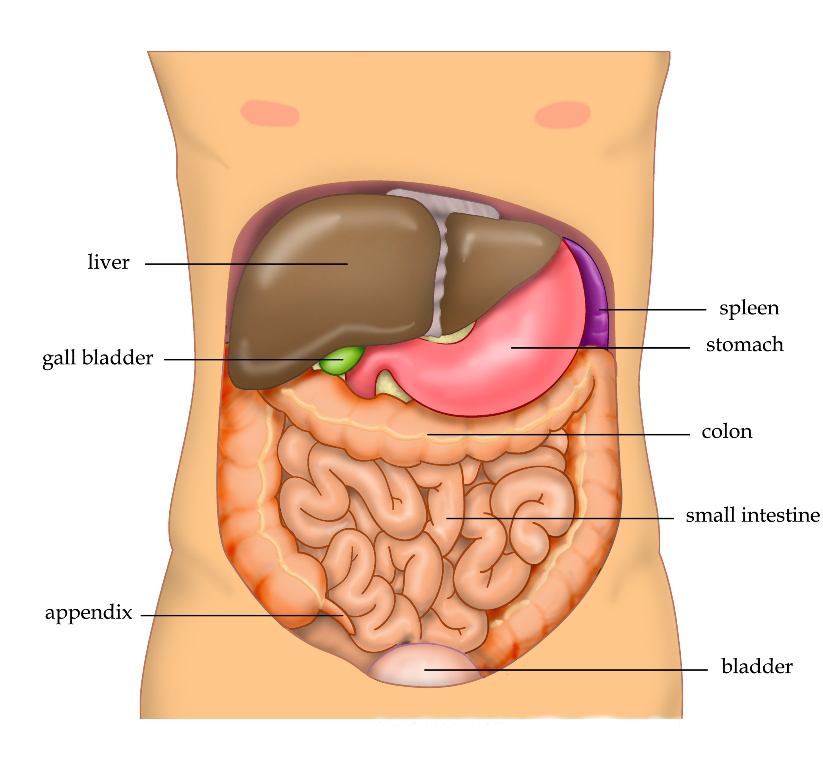
\includegraphics[width = 0.75\columnwidth]{./Images/Chapter1/liverIllustration.jpg}%
\caption{The human liver.}
\label{fig:Ch1LiverAnatomy}
\end{figure}    

Liver cancer is a significant health concern in the United States. Liver cancer can be subdivided into primary liver cancer, where the disease originates in the cells of the liver, and secondary liver cancer, where the cancer originates in other organs and metastasizes to the liver. Approximately 35,660 new cases of primary liver cancer will be diagnosed in the United States in 2015, and approximately 24,550 people will die of these cancers~\cite{AmericanCancer2015}. Secondary liver cancers occur more frequently. Common types of cancer such as breast, lung, and colon all metastasize to the liver. For example, a quarter of the approximately 130,000 patients diagnosed with colorectal cancer each year in the United States will develop liver metastases~\cite{Ananthakrishnan2006,CDC2015,Haddad2011}. Liver cancer is an even more significant health concern in other parts of the world. Liver cancer is the most common type of cancer in many countries in sub-Saharan Africa and Southeast Asia. More than 700,000 people are diagnosed with this cancer each year throughout the world, with more than 600,000 deaths annually~\cite{AmericanCancer2015}.

\subsection{Treatment of Liver Tumors}
Surgery, either for resection of the tumor or a liver transplant, is the only curative treatment of liver cancer, and offers the best long-term survival in select patients. However, approximately three quarters of patients are ineligible for surgery due to tumor size, type, or location; inadequate liver reserve; or other comorbidities. Percutaneous radiofrequency ablation (RFA) is a common, less invasive treatment option for liver cancer patients who are not eligible for resection or transplantation. In this procedure, long electrodes are inserted through the skin into the liver, and are used to ablate the cancer by depositing a high-frequency alternating current into the tissue. 

Current percutaneous RFA of liver cancer suffers from significant limitations~\cite{Gervais2009}. Straight electrodes are unable to reach tumors in some portions of the liver because they are blocked by vasculature, lung, or other sensitive structures. Large tumors require multiple electrode insertions, with each puncture through the liver capsule increasing the risk of hemorrhage. This increased risk can make patients with advanced liver disease or severe comorbidities ineligible for the RFA procedure. Successful treatment requires a margin of cancer-free tissue to be ablated around the tumor, in order to reduce the likelihood of recurrence~\cite{Kim2006}. For medium to large tumors, developing a sufficient ablative margin is highly dependent on the clinician's ability to locate the electrode tip over multiple passes using medical imaging for guidance~\cite{Dodd2001}. 

\subsection{Robotic Needle Steering}
Robotic needle steering enables the insertion of flexible needles along controlled, curved, three-dimensional (3D) paths through tissue~\cite{DiMaio2005,Webster2006}. Robotic needle steering offers the potential to improve percutaneous RFA of liver tumors in several ways. Specifically, robotic needle steering may allow clinicians to (1) correct for errors during insertion and reach a target position with superior accuracy compared to manual insertion, (2) steer around obstacles to previously unreachable targets, and (3) reach multiple targets from a single insertion site, thus reducing the risk of complications such as hemorrhage or infection.

%%%%%%%%%%%%%%%%%%%%%%%%%%%%%%%%%%%%%%%%%%%%%%%%%%%%%%%%%%%%%%%%%%%%%%%%%%%%%%%%%%%%%%%%%%%%%%%%%%%%======================================================================
\section{Prior Work}
%======================================================================
%%%%%%%%%%%%%%%%%%%%%%%%%%%%%%%%%%%%%%%%%%%%%%%%%%%%%%%%%%%%%%%%%%%%%%%%%%%%%%%%%%%%%%%%%%%%%%%%%%%

\subsection{Techniques for Needle Steering}
A number of methods have been described for steering needles through tissue. A recent review is given in~\cite{vandeBerg2014}. DiMaio and Salcudean~\cite{DiMaio2005} and Glozman and Shoham~\cite{Glozman2007} used lateral robotic manipulation of the needle base during insertion to steer the needle. Mallapragada et al.~\cite{Mallapragada2009} and Torabi et al.~\cite{Torabi2009} used robotic manipulation of simulated tissues around a needle during insertion to steer the needle. Okazawa et al.~\cite{Okazawa2005} used a precurved stylet that could be rotated and translated relative to a straight needle shaft to steer a manually inserted needle device. The same concept of overlapping pre-curved sections has been applied in multiple stages in the active cannula robots described by Sears and Dupont~\cite{Sears2006} and Webster et al.~\cite{Webster2009}. Kratchman et al.~\cite{Kratchman2011} described tendon actuation systems designed to steer flexible needle shafts in solid tissue. Ayvali et al.~\cite{Ayvali2012}, Datla et al.~\cite{Datla2014}, and Ryu et al.~\cite{Ryu2014} have described using shape memory alloy (SMA) actuators to articulate needle sections, with the latter system using optically actuated SMA tendons to allow compatibility with MRI systems. Ko and Rodriguez y Baena~\cite{Ko2013} have described a biologically inspired needle that steers by adjusting the relative offset between parallel sections. Our work focuses on bent-tip steerable needles: flexible needle shafts with bent distal sections. These needles naturally steer along curved paths during insertion as a result of the net lateral force acting at the distal end of the needles~\cite{Webster2006}. A duty-cycle control approach, first proposed by Minhas et al.~\cite{Minhas2007}, allows curvature to be varied by alternating periods of needle rotation. A bent-tip needle with a passive flexure was introduced by Swaney et al.~\cite{Swaney2013} to reduce tissue damage caused by the bent tip during rotation. Similar flexible needles with bevel tips~\cite{OLeary2003,Alterovitz2005} and curved distal sections~\cite{Wedlick2009} have also been described. A tendon-actuated bent-tip steerable needle was described by van de Berg et al.~\cite{vandeBerg2015}. This design incorporates a two degree-of-freedom ball and socket joint with a conical tip to achieve 3D steering.

\subsection{Automatic Segmentation of Needles from Ultrasound}
A large amount of prior art exists on the automatic segmentation of needles from B-mode (grayscale) ultrasound data, with much of it focused on segmenting straight needles using a variant of the Hough transform. Although the Hough transform is computationally intensive, real-time segmentation of straight needles has been demonstrated using variations on the algorithm, including dual-plane projections~\cite{Ding2003b}, coarse-fine sampling~\cite{Ding2003a,Zhou2008}, and parallel implementation on a graphics processing unit~\cite{Novotny2007}. Other similar algorithms, such as the parallel integral projection transform, have also been applied~\cite{Barva2008}. Similar methods have been described for segmenting curved needles. Slightly curved needles can be segmented using a standard Hough transform method~\cite{Okazawa2006,Aboofazeli2009}, while more strongly curved needles can be segmented by including a parametrization of needle bending~\cite{Neshat2008,Okazawa2006,Uhercik2010}.

The underlying issue that makes automatic needle segmentation a difficult problem is the poor visibility of needles in standard B-mode ultrasound data. Several of the described methods have shown promising results in favorable conditions. However, image-guided robotic needle steering requires segmentation algorithms that can process large 3D datasets containing highly curved, extremely thin (e.g., 0.5-mm diameter) needles at undesirable orientations relative to the transducer. Rather than contribute a new algorithm that attempts to overcome these challenges, our aim in this work was to reduce the complexity of the segmentation task, by leveraging the needle steering robot to produce ultrasound image data that more clearly reveal the needle.

\subsection{Doppler-Based Segmentation}
Ultrasound Doppler is a diagnostic technique that measures frequency shifts in reflected ultrasonic waves that result from motion. Color and power Doppler imaging, which are available on most modern ultrasound systems, are commonly applied to overlay blood flow data on B-mode ultrasound. Vibrating solid objects have also been shown to produce recognizable Doppler signals~\cite{Holen1985}. This concept has been applied to localize straight needles~\cite{Armstrong2001,Feld1997,Hamper1991} and needle tips~\cite{Harmat2006} in 2D ultrasound, as well as instruments in cardiac interventions~\cite{Fronheiser2008,Reddy2008} and other applications~\cite{McAleavey2003,Rogers2009}. This technique has not previously been applied to segment highly curved needles.

\subsection{Control Approaches for Robotic Needle Steering}
There is significant prior art relevant to image-guided control of needle steering, both for bent-tip steerable needles and other approaches. DiMaio and Salcudean formulated rigid needle insertion as a trajectory planning and control problem, defining a needle manipulation Jacobian for base control~\cite{DiMaio2005}. Glozman and Shoham~\cite{Glozman2007} and Neubach and Shoham~\cite{Neubach2010} used inverse kinematics to control base-manipulation needle steering, with X-ray and ultrasound image feedback respectively. Ko and Rodriguez y Baena used a model-predictive control algorithm for trajectory-following control of a bio-inspired actuated flexible needle~\cite{Ko2012}. For bent-tip steering, a number of control approaches have been described based on a nonholonomic model of steerable needle motion in tissue~\cite{Webster2006}. Reed et al. demonstrated image-guided needle steering in a planar workspace~\cite{Reed2011}, by combining a planar motion planner~\cite{Alterovitz2008}, an image-guided controller~\cite{Kallem2009}, and a torsion compensator~\cite{Reed2009}. Wood et al. formulated trajectory tracking controllers based on duty cycling for 2D~\cite{Wood2010} and 3D~\cite{Wood2013} trajectories. Bernardes et al. combined closed-loop image feedback with intraoperative replanning to deal with obstacles and dynamic workspaces~\cite{Bernardes2013}. Rucker et al.~\cite{Rucker2013} used a sliding mode controller with feedback from an electromagnetic tracking system. This control scheme has the advantage that it does not require any prior knowledge of needle curvature. Abayazid et al. demonstrated bent-tip needle control in gelatin and chicken breast using a robotically controlled ultrasound transducer to track the tip~\cite{Abayazid2014}. The steerable needle described by van de Berg et al.~\cite{vandeBerg2015} uses an integrated fiber Bragg grating (FBG) shape sensor and proportional-integral control of the tendon-actuated tip. 

Several schemes for teleoperation or human-in-the-loop control of steerable needles have been proposed. Romano et al. implemented several joint-space control schemes, comparing autonomous, manual, and combined control of the insertion and rotation of the steerable needle~\cite{Romano2007}. Majewicz and Okamura implemented task-space teleoperation using a 3D display and a haptic device as a master input~\cite{Majewicz2013}. In a human user study, they found task-space teleoperation resulted in lower time to target and insertion length than joint-space teleoperation. Pacchierotti et al. implemented a teleoperation system that combined kinesthetic and
vibratory feedback to provide information about ideal insertion and rotation of the steerable needle~\cite{Pacchierotti2014}.

\subsection{Current State of Needle Steering Research}
Robotic needle steering has existed solely as a research concept for over a decade. The work on rigid needle steering by DiMaio and Salcudean in 2005~\cite{DiMaio2005} appears to be the first in this area. At roughly the same time, Webster et al. suggested using flexible needles with asymmetric tips to steer through solid organs~\cite{Webster2005}. Since then there have been dozens of journal and conference articles on this topic, all motivated by the potential benefits of achieving controlled, curved needle paths through tissue. Interestingly for a medical robotics topic, there has been almost no progression towards clinical or patient studies. Steerable needles have only been applied in one \textit{in vivo} test~\cite{Majewicz2012}, which measured open-loop steerable needle curvature in different tissues, without simulating any clinical scenario or performing any closed-loop targeting.

To date, needle steering research has been largely the domain of roboticists. Experimental validation of many of the methods described above have been limited to artificial tissues. These artificial tissues provide only limited validation, as their mechanical properties are significantly different from biological tissues~\cite{Wedlick2012}. Without methods for medical image feedback, many needle steering experiments have been constrained to 2D workspaces in transparent artificial tissues such as agar or PVC rubber, with optical cameras used to simulate medical imaging. Although some studies have applied more realistic medical imaging methods~\cite{Glozman2007,Neubach2010,Abayazid2014}, they have generally been evaluated in tightly controlled bench-top settings, yielding best-case needle visibility.

The high-level goal of this thesis was to move robotic needle steering closer to the clinical domain, by targeting a specific percutaneous intervention (ablation of liver tumors), and solving several of the largest technical problems specific to that procedure. In particular, we focused on implementing real-time medical image feedback, achieving sufficient curvature in liver tissue, and allowing human-in-the-loop control. In all these areas, our focus was on clinically realistic implementations that were validated in biological tissues.  

%%%%%%%%%%%%%%%%%%%%%%%%%%%%%%%%%%%%%%%%%%%%%%%%%%%%%%%%%%%%%%%%%%%%%%%%%%%%%%%%%%%%%%%%%%%%%%%%%%%%======================================================================
\section{Contributions}
%======================================================================
%%%%%%%%%%%%%%%%%%%%%%%%%%%%%%%%%%%%%%%%%%%%%%%%%%%%%%%%%%%%%%%%%%%%%%%%%%%%%%%%%%%%%%%%%%%%%%%%%%%
The major contributions of the research described in this dissertation can be summarized as follows:
\begin{itemize}
\item Proposed and validated a method for automatic segmentation of a steerable needle from 3D ultrasound data, based on applying mechanical vibration to the steerable needle in order to make it visible in power Doppler ultrasound.
\item Completed a workspace analysis of percutaneous RFA of liver tumors, using medical image analysis to set a procedure-specific requirement for steerable needle curvature.  
\item Performed finite-element modeling and experimental studies to demonstrate that the required steerable needle curvature can be achieved in liver tissue through optimization of tip geometry. Motivated by these results, proposed and validated an articulated-tip steerable needle mechanism.   
\item Implemented and validated a system for freehand-3D-ultrasound-guided needle steering, which allows a clinician to manually visualize target anatomy while simultaneously providing image feedback for automatic control. Proposed and validated an estimation scheme based on an unscented Kalman filter. 
\end{itemize}

%%%%%%%%%%%%%%%%%%%%%%%%%%%%%%%%%%%%%%%%%%%%%%%%%%%%%%%%%%%%%%%%%%%%%%%%%%%%%%%%%%%%%%%%%%%%%%%%%%%%======================================================================
\section{Dissertation Overview}
%======================================================================
%%%%%%%%%%%%%%%%%%%%%%%%%%%%%%%%%%%%%%%%%%%%%%%%%%%%%%%%%%%%%%%%%%%%%%%%%%%%%%%%%%%%%%%%%%%%%%%%%%%
This dissertation is composed of six chapters. This introductory chapter has provided the clinical motivation for the work, a survey of relevant research literature, and a summary of the contributions of the dissertation. Chapter 2 describes methods for automatic segmentation of a steerable needle from 3D ultrasound data. Chapter 3 describes the workspace analysis of percutaneous RFA of liver tumors, as well as finite-element modeling, experimental studies and mechanism design intended to achieve improved steerable needle curvature in liver tissue. Chapter 4 describes a new estimation scheme based on an unscented Kalman filter, which is used to improve closed-loop steering results with noisy ultrasound measurements.
Chapter 5 combines elements from the previous chapters, in order to demonstrate human-in-the-loop control of ultrasound-guided needle steering. Finally, Chapter 6 summarizes the results of the research, reviews the contributions made in this dissertation, and provides suggestions for future work.
%!TEX root = PhD_Thesis.tex
\chapter[Segmentation from 3D Ultrasound]{Segmentation of Steerable Needles from 3D Ultrasound Image Data}

%%%%%%%%%%%%%%%%%%%%%%%%%%%%%%%%%%%%%%%%%%%%%%%%%%%%%%%%%%%%%%%%%%%%%%%%%%%%%%%%%%%%%%%%%%%%%%%%%%%%======================================================================
\section{Introduction}
%======================================================================
%%%%%%%%%%%%%%%%%%%%%%%%%%%%%%%%%%%%%%%%%%%%%%%%%%%%%%%%%%%%%%%%%%%%%%%%%%%%%%%%%%%%%%%%%%%%%%%%%%%
This chapter describes methods for automatic segmentation of steerable needles from 3D ultrasound data. The work presented in this chapter was previously published in the IEEE Transactions on Biomedical Engineering~\cite{Adebar2014}.

CT imaging, magnetic resonance (MR) imaging and X-ray imaging could all potentially be applied to intraoperative guidance of steerable needles, but each of these modalities has significant drawbacks. Our work uses 3D ultrasound because of its many advantages. Ultrasound systems image in real time, do not produce ionizing radiation, and are not strongly affected by the presence of metal objects such as needles. Perhaps most importantly, ultrasound systems are inexpensive and portable, and are already standard equipment in existing operating rooms and treatment suites.  

Ultrasound does have disadvantages, such as low signal-to-noise ratio and poor image resolution compared to MR or CT. When imaging needles, ultrasound image quality is highly dependent on the angle between the ultrasound imaging plane and the needle. At some angles, significant reverberation artifacts generated by the highly reflective needle surfaces may appear. At other angles, the needle may not be visible at all, as the reflected waves may be dispersed away from the transducer~\cite{Chung2004}. Even when the needle can be identified, various imaging artifacts can make it difficult to locate the tip of the needle along its axis. 

The underlying issue that makes automatic needle segmentation a difficult problem is the poor visibility of needles in standard B-mode ultrasound data. Several methods for B-mode segmentation have shown promising results in favorable conditions. However, image-guided robotic needle steering requires segmentation algorithms that can process large 3D datasets containing highly curved, extremely thin (e.g., 0.6-mm diameter) needles at undesirable orientations relative to the transducer. Rather than contribute a new algorithm that attempts to overcome these challenges, our aim in this chapter was to reduce the complexity of the segmentation task, by leveraging the needle steering robot to produce ultrasound image data that more clearly reveal the needle.

Ultrasound Doppler is a diagnostic technique that measures frequency shifts in reflected ultrasonic waves that result from motion. Color and power Doppler imaging, which are available on most modern ultrasound systems, are commonly applied to overlay blood flow data on B-mode ultrasound, as described in Section~\ref{sec:Doppler-BasedSegmentation}. Vibrating solid objects have also been shown to produce recognizable Doppler signals~\cite{Holen1985}. This concept has been applied to localize straight needles~\cite{Armstrong2001,Feld1997,Hamper1991} and needle tips~\cite{Harmat2006} in 2D ultrasound, as well as instruments in cardiac interventions~\cite{Fronheiser2008,Reddy2008} and other applications~\cite{McAleavey2003,Rogers2009}. This technique has not previously been applied to segment highly curved needles.

\begin{figure}[!t]
\centering
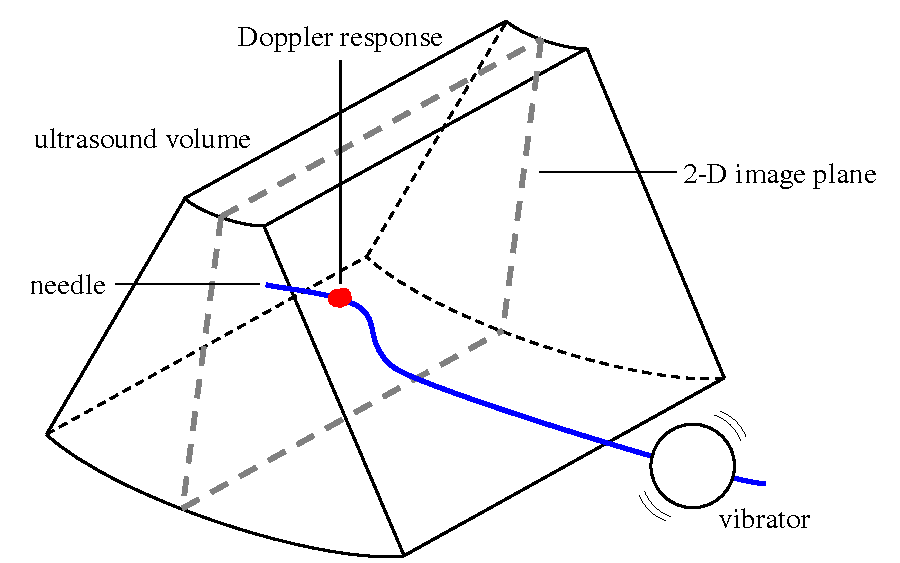
\includegraphics[width = 0.75\columnwidth]{Images/Chapter2/SliceConcept/SliceConcept}%
\caption[3D ultrasound segmentation concept]{Needle segmentation concept. A voice coil actuator (vibrator) vibrates the needle, resulting in a Doppler response around the needle cross section in a 2D ultrasound image. The needle is segmented by localizing the Doppler response across the sweep of a mechanical 3D ultrasound transducer, and fitting a curve through the resulting points.}
\label{fig:SliceConcept}
\end{figure}

The remainder of this chapter is divided into four sections. Section~\ref{sec:Algorithms} describes our Doppler segmentation approach. Section~\ref{sec:Closed-loopControlDoppler} describes a closed-loop control approach, which incorporates the segmentation results as feedback. Variations of this control approach will also be applied in later chapters. Section~\ref{sec:ExperimentalValidation} describes experimental methods for validation of our segmentation and control algorithms. Section~\ref{sec:Results} presents and discusses the results of the validation testing.

\section{Segmentation Algorithm}
\label{sec:Algorithms}
Throughout the description of our segmentation algorithm, we will assume that the needle is oriented roughly orthogonal to the imaging plane of a mechanical 3D ultrasound transducer, as depicted in Fig.~\ref{fig:SliceConcept}. An actuator is used to vibrate the needle, and the resulting motion of the needle and surrounding tissue produces a Doppler signal across the series of $N$ Doppler images generated by the ultrasound system. Segmentation proceeds in two stages, as depicted in Fig.~\ref{fig:Segmentation}. First, the cross section of the needle is localized in each image through 2D image processing. Second, the 3D shape of the needle is reconstructed by fitting a curve to the series of points.

\subsection{2D Image Processing}
To remove Doppler noise, patches with less than 300 connected pixels are removed. (For comparison, the Doppler patch centered around the needle typically has a connected area of 1000 to 2000 pixels.) After this preprocessing step, the image coordinates of the needle cross section are estimated based on the remaining Doppler response. As seen in the example image in Fig.~\ref{fig:Segmentation}, the Doppler response from the vibration generally appears as an irregular, roughly circular patch centered on the needle, with a color comet tail artifact in the axial ($y_\text{image}$) direction~\cite{Tchelepi2009}. The lateral ($x_\text{image}$) coordinate of the needle is thus estimated as the centroid of the Doppler response. To account for the color comet tail, the axial image coordinate of the needle is estimated as the point that separates one quarter of the integral of the Doppler response above, and three quarters below. These fractions were selected empirically based on the results of our feasibility study~\cite{Adebar2013}. 

We define the $x$, $y$, and $z$ directions of the 3D ultrasound coordinate system to be in the lateral, axial, and elevational directions, respectively. Based on the geometry of the ultrasound transducer, the needle points are mapped from the 2D image coordinate system to the 3D ultrasound coordinate system, yielding the set of $N$ needle points $d^{(0)}, \dotsc, d^{(N)}$. Each $d^{(i)} \in \mathbb{R}^{3}$ holds the $x$-$y$-$z$ coordinates of detected needle point~$i$.

\begin{figure*}[!t]
\centering
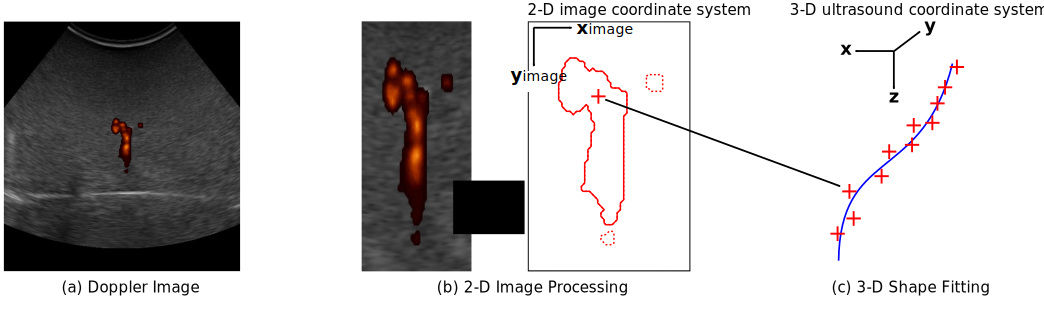
\includegraphics[width = \textwidth]{Images/Chapter2/Segmentation/Segmentation}%
\caption[Doppler ultrasound segmentation algorithm]{Segmentation algorithm: (a) Doppler image. A 2D ultrasound Doppler image from a series of $N$ captured over a sweep of the imaging plane. (b)~2D image processing. Doppler patches with fewer than 300 connected pixels are assumed to be noise and discarded (dotted lines). The remaining Doppler data (solid line) are used to estimate the position of the needle cross section (cross). In the lateral ($x_\text{image}$) direction, the position is estimated as the centroid of the Doppler response. In the axial ($y_\text{image}$) direction, the position is estimated as the lower bound of the region that contains one quarter of the integrated Doppler intensity. (c) 3D shape fitting. The 2D-localized points are combined in 3D based on position information from the 3D ultrasound transducer. Third-order polynomial curves are fit to the identified points in order to define the needle's 3D shape over the series of $N$ images.}
\label{fig:Segmentation}
\end{figure*}

\subsection{3D Shape Fitting}
Based on the Doppler points identified in the previous step, we resolve the shape of the needle by defining the $x$ and $y$ coordinates as functions of the $z$ coordinate over the range of $d^{(0)}, \dotsc, d^{(N)}$. In this work we use third-order polynomial functions,
\begin{align}
d^{(i)}_x = f_x(d_z^{(i)}) = a_0 + a_1(d_z^{(i)}) + a_2(d_z^{(i)})^{2} + a_3(d_z^{(i)})^{3},\notag\\
d^{(i)}_y = f_y(d_z^{(i)}) = b_0 + b_1(d_z^{(i)}) + b_2(d_z^{(i)})^{2} + b_3(d_z^{(i)})^{3},\label{result}
\end{align}
and solve for the vectors of polynomial coefficients $a,b \in \mathbb{R}^{4}$ that minimize the sum of the squared error over the measured Doppler points. We selected this curve type because a third-order polynomial was sufficient to represent the range of curved needle paths we considered in this study. Additionally, low-order polynomials have the advantage that they average out noise in the 2D Doppler points, which is important in our method. Longer, more tortuous paths might require more sophisticated curves, possibly segmented polynomials constrained to be tangent at transition points.

\begin{figure}[!t]
\centering
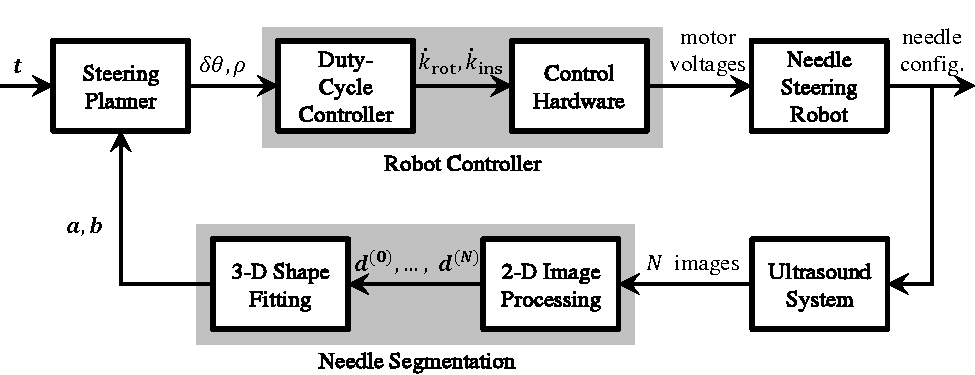
\includegraphics[width=\columnwidth]{Images/Chapter2/ControlBlockDiagram/ControlBlockDiagram}%
\caption[Block diagram of closed-loop control algorithm]{Block diagram of closed-loop control in ultrasound-guided needle steering. Automatic segmentation of the needle from 3D ultrasound data provides a measurement of needle tip pose to a steering controller, which identifies the needle rotation and curvature necessary to reach a target point. A duty-cycle controller generates the velocity commands that allow motor control hardware to move the needle tip along the desired path to the target.}
\label{fig:ControlBlockDiagram}
\end{figure}

\section{Closed-loop Control Algorithm}
\label{sec:Closed-loopControlDoppler}
To demonstrate the usefulness of the Doppler ultrasound segmentation method described in the previous section, we implemented closed-loop control of a needle steering robot using the ultrasound segmentation results as feedback. Fig.~\ref{fig:ControlBlockDiagram} shows a block diagram. The goal of the closed-loop control is to steer the needle tip towards a target point ${t}$ defined in the ultrasound coordinate system. The same general framework for closed-loop control will be used in Chapters 4 and 5, with some modifications. Implementation of closed-loop control necessitated two new algorithmic components in addition to needle segmentation: tip pose measurement and a steering controller. 

The pose of the needle tip, defined by position $p$ and orientation $R$, is measured by interpreting the needle segmentation results. In this chapter, the tip pose measurement is based on a small-angle approximation. This approximation is appropriate for the range of needle steering paths described in this chapter, which are representative of ablation shaping around a single tumor. In Chapter 4, we describe an estimation scheme based on an unscented Kalman filter, which allows position feedback to be combined with a kinematic model of needle tip motion, in order to estimate the complete tip pose. This estimation scheme enables longer paths steering through a large workspace in the liver. 

The steering controller interprets the tip pose measurement, and determines a desired path for the steerable needle that will cause it to reach the target. In this chapter, a simple replanning approach, previously described by Majewicz and Okamura~\cite{Majewicz2013}, was employed. This approach has the limitation that it requires duty-cycle control of needle curvature; however, it is sufficient to demonstrate accurate closed-loop steering for the small paths described in this chapter. In Chapter 5, we apply the sliding mode control described in~\cite{Rucker2013}, which does not rely on duty-cycle control.

The tip frame measurement algorithm and steering controller, as well as the robotic system used to validate them, are described in detail in the remainder of this section. 

\subsection{Tip Pose Measurement}
We define the needle tip frame as shown in Fig.~\ref{fig:ControlAlgorithm}. The origin of the tip frame is located at point ${p}$, which is the distal end of the needle. For simplicity, we ignore the local geometry of the bent tip. The tip frame has orientation represented by rotation matrix $R$, with the $z_{\text{tip}}$ axis tangent to the needle at ${p}$, and the $y_{\text{tip}}$ axis pointing in the direction of curvature. The center of curvature for the circular needle path ${c}$ lies on the $y_{\text{tip}}$-axis, at a distance $\rho$ from ${p}$. Using duty-cycle control~\cite{Minhas2007}, $\rho$ can be varied from $\rho_{\text{min}}$ to $\infty$ (a straight line).  

%In our model, rotating the base of the needle by $\delta\theta$ causes the needle tip frame to rotate by $\delta\theta$ about the $z_{\text{tip}}$ axis, while inserting the needle causes the tip point ${p}$ to move along  a circular path of radius $\rho$.

Based on the segmentation result, the tip point ${p}$ is identified using the $z$ coordinate of the most distal Doppler point and the polynomial curve functions,
\begin{align}
{p} = \begin{bmatrix}p_x & p_y & p_z\end{bmatrix}^{\text{T}} = \begin{bmatrix}f_x(d^{(0)}_z) & f_y(d^{(0)}_z) & d^{(0)}_z \end{bmatrix}^{\text{T}}.
\end{align}
While it should also be possible to estimate the tip frame orientation $R$ based on the needle segmentation result, for example by fitting a circular arc to a curved section of the 3D segmentation result to define the steering direction, we have found that in the current implementation the Doppler segmentation results are too noisy to allow reliable estimation of the tip frame orientation. Instead we apply a small angle approximation, and assume that the $z_{\text{tip}}$ axis remains close to the $z$ axis of the 3D ultrasound coordinate system throughout steering. The orientation of the tip frame can thus be specified completely by a rotation of $\theta$ about the $z$ axis. We make rotation angle $\theta$ a system variable, and update it after each iteration of the steering controller, 
\begin{align}
\theta_\text{i+1} = \theta_\text{i} + \delta\theta_\text{i}.
\end{align}
This approach ignores torsional deflection of the steerable needle as result of friction between the needle and tissue. While substantial torsional deflection has been demonstrated in artificial tissues, in biological tissues the needle tip rotation has been shown to follow the base rotation to within a few degrees~\cite{Reed2008}. 

\subsection{Steering Controller}
At each iteration, the steering controller interprets the tip pose measurement, defined by $p$ and $R$, and identifies the simplest possible path to the target point ${t}$. As shown in Fig.~\ref{fig:ControlAlgorithm}, this path is the circular arc that is tangent to the measured $z_{\text{tip}}$ axis at $p$, and passes through ${t}$. The radius of the desired path $\rho_{\text{des}}$ and the incremental needle rotation $\delta\theta$ needed to follow the path are output to the robot controller, which drives the motors of the needle steering robot.

\begin{figure}[!t]
\centering
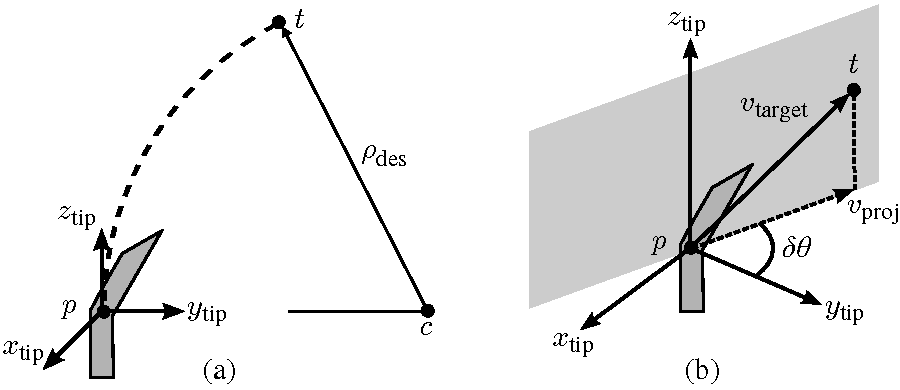
\includegraphics[width = 0.75\columnwidth]{Images/Chapter2/ControlAlgorithm/ControlAlgorithm}%
\caption[Steering controller]{Steering controller: (a) The needle tip frame is located at the distal end of the needle. The frame is oriented with the $z_{\text{tip}}$ axis tangent to the needle, and the $y_{\text{tip}}$ axis pointing towards the center of curvature. The needle follows a circular path, with radius $\rho$ which can be varied using duty-cycle control. (b) The steering controller determines the incremental rotation $\delta\theta$ and the desired path radius $\rho_{\text{des}}$ that will cause the needle tip $p$ to reach the target point ${t}$.}
\label{fig:ControlAlgorithm}
\end{figure}

\subsection{Robot Controller} 
The robot controller consists of two components. A duty-cycle controller generates motor velocity commands based on the desired needle rotation and radius of curvature as output by the steering controller. Motor control hardware drives the motors of the needle steering robot based on the velocity commands.

\subsubsection{Duty-Cycle Controller}
The goal of the duty-cycle controller is to determine the desired velocities for the rotation and insertion stages, $\dot{k}_\text{rot}$ and $\dot{k}_\text{ins}$. It is first necessary to calculate the duty-cycle fraction $DC$, based on the desired radius of curvature. Assuming a known minimum radius of curvature $\rho_\text{min}$ for the specific needle-tissue pair, $DC$ can be calculated as,
\begin{align}
DC = 1.0 - \frac{\rho_\text{min}}{\rho_{\text{des}}}. 
\label{eq:DC}
\end{align}
The insertion velocity, $\dot{k}_\text{ins}$, is set to a constant value during steering.  To achieve the duty-cycle effect, the rotation stage alternates between constant velocity, $\dot{k}_\text{rot} = \dot{k}_\text{rot, max}$, and zero velocity, $\dot{k}_\text{rot} = 0$, with the needle held at angle $\theta$. The ratio of time spent rotating ($T_\text{rot}$) to time holding at angle $\theta$ ($T_\text{hold}$) is determined from the duty cycle ratio $DC$,
\begin{align}
DC =\frac{T_\text{rot}}{T_\text{rot}+T_\text{hold}}.
\end{align}
Rotation time $T_\text{rot}$ is constant and equal to the time required to complete a full rotation. Hold time $T_\text{hold}$ is thus varied to achieve the desired ratio $DC$.

\subsubsection{Control Hardware}
There are many possible hardware implementations that could be used to drive the motors of the needle steering robot. In the system we use for experimental validation in Section~\ref{sec:ExperimentalValidation}, the rotation and insertion motors are each driven by integrated motion control systems. These systems accept velocity commands (i.e., $\dot{k}_\text{rot}, \dot{k}_\text{ins}$) and drive the motors using proportional-integral (PI) control. In our system, PI control constants were tuned using manufacturer supplied software.

\section{Experimental Validation}
\label{sec:ExperimentalValidation}
In this section, we describe experimental validation of our algorithms for segmentation and closed-loop 3D ultrasound-guided needle steering.
\subsection{Apparatus}
%Figure~\ref{fig:Setup} shows our experimental apparatus.
\subsubsection{Ultrasound Imaging}
A SonixMDP ultrasound console (Ultrasonix Medical Corp., Richmond, Canada) with a convex mechanical 3D transducer (4DC7-3/40) was used for imaging. Custom software incorporating the Ultrasonix research SDK package was used to control imaging parameters and capture images. Power Doppler imaging mode was selected over color Doppler imaging because of the lack of aliasing and reduced sensitivity to imaging angle. Pulse repetition frequency (PRF) was set to 1428 Hz, as this setting yielded the best results in our initial feasibility study~\cite{Adebar2013}. Wall motion filter (WF) was set to maximum in order to minimize Doppler artifacts resulting from the motion of the imaging plane. Each sweep consisted of 61 scan-converted 2D images, captured at angular increments of approximately 0.7 degrees.

\begin{figure*}[!t]
\centering{
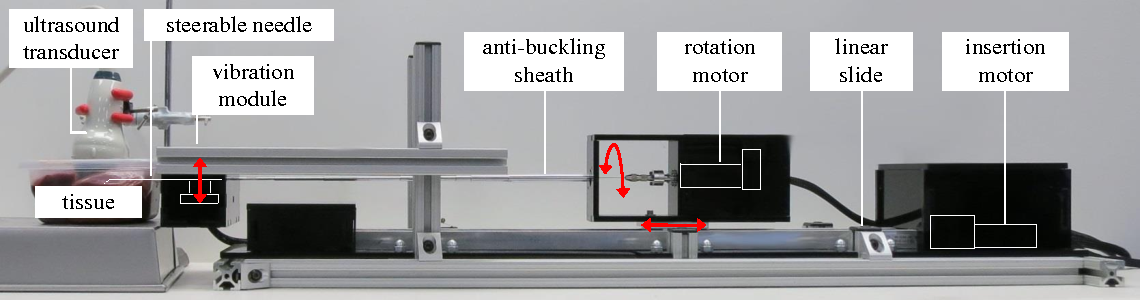
\includegraphics[width=\textwidth]{Images/Chapter2/RobotSetup/RobotSetup}%
}
\caption[Experimental setup]{Experimental setup. Needle steering robot consisting of actuated linear slide, rotation stage, and vibration module (red arrows indicate actuation); \textit{ex vivo} bovine liver tissue; 3D ultrasound transducer.}
\label{fig:ExperimentalSetup}
\end{figure*}

\begin{figure}[!t]
\centering{
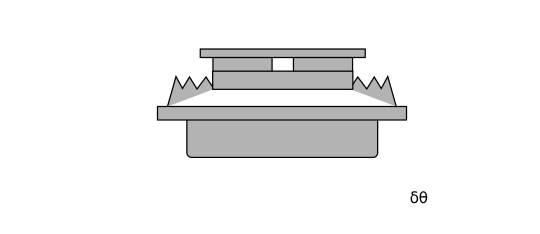
\includegraphics[width = 0.7\columnwidth]{Images/Chapter2/Vibrator/Vibrator}%
}
\caption[Vibration module]{Vibration module. A voice coil actuator is attached to the steerable needle using a 3D-printed clip, and used to vibrate the needle vertically (in and out of the page).}
\label{fig:Vibrator}
\end{figure}

\subsubsection{Needle Steering Robot}
Fig.~\ref{fig:ExperimentalSetup} shows the needle steering robot used to validate our control method. Similar to previously described needle steering robots~\cite{Webster2005}, our system has two active degrees of freedom (DOF) that control needle insertion and needle rotation. Unlike previous needle steering robots, our system incorporates a vibration module that generates the high-frequency motion necessary to visualize the needle using ultrasound Doppler.

The rotational DOF is actuated by a geared DC motor (A-max 22-110160; Maxon Motor, Sachseln, Switzerland) that is connected directly to the needle through a pin-vise clamp. The insertion DOF is actuated by a DC motor (GM9234S016; Ametek, Berwyn, PA) that drives a linear slide (SPMA2524W4; VelMex, Bloomfield, NY). Both the rotation DOF and insertion DOF are driven by integrated motion controllers (MCDC3006S; Faulhaber, Schönaich, Germany). The vibration module, shown in Fig.~\ref{fig:Vibrator}, consists of a voice coil actuator (HIAX19C01-8; HiWave, Little Gransden, UK) that is driven by a transistor circuit at a user-variable frequency of 400~Hz, 600~Hz or 800~Hz. These frequencies are roughly centered around the peak output point of the voice coil actuator and thus produce the strongest responses in the power Doppler image data. To produce the maximum vibration along the needle, the vibration module was designed to be as close as possible to the target tissue, and is thus attached to the distal end of the needle steering robot. The needle is mated to the actuator using a 3D-printed plastic clip.

\subsubsection{Needles}
Solid Nitinol wires 0.38~mm (0.015~inches), 0.48~mm (0.019~inches) and 0.58~mm (0.023~inches) in diameter were used as needles. The needles had 45-degree beveled tips and 4.5-mm distal sections bent 35 degrees off axis.

\subsubsection{Tissue Simulant}
\textit{Ex vivo} bovine liver tissue obtained fresh from a local butcher was used as the tissue simulant in all testing.

\subsection{Segmentation Accuracy}
We previously described a feasibility study~\cite{Adebar2013}, in which we measured the accuracy of our Doppler segmentation method using piezoelectric elements welded to stainless-steel wires. In that study, we examined the sensitivity of the method to tissue composition, vibration frequency, and Doppler PRF, and found that only PRF greatly affected the accuracy of segmentation. Based on comparison with manual segmentation, we found the average error to be 1 to 2~mm across most conditions.

In this study, we evaluated the accuracy of segmentation when using an actual needle steering robot with an integrated actuator to vibrate flexible Nitinol needles. We again considered the impact of vibration frequency, although at a lower range than our previous experiment because of the lower center frequency of the voice coil actuator compared to the previous piezoelectric actuator. We also considered the impact of needle curvature, needle diameter, and position of the needle in the lateral image direction. Two needle curvatures (straight and maximum curvature), two lateral positions (image center and lateral edge), three needle diameters (0.38~mm, 0.48~mm, and 0.58~mm), and three vibration frequencies (400~Hz, 600~Hz, and 800~Hz) were tested. Each parameter was varied individually around the base case of a straight, 0.48-mm needle centered in the image and vibrated at 600~Hz. 

Three separate insertions and scans were performed for each test condition. Segmentation accuracy was evaluated by comparison with a reference manual segmentation of the needle from B-mode data, within the native image planes of the 3D ultrasound transducer. To create the reference data, the center of the needle was manually selected in each 2D B-mode image in which it was visible. The needle was visible in approximately 50 percent of the B-mode images captured over most sweeps. 

Given $K$ manually selected needle points ${m}^{(0)}, \dotsc, {m}^{(K)}$, we defined the segmentation error for the $i$-th point,
\begin{equation}
e^{(i)} = \sqrt{ \left(m_x^{(i)}-f_x(m_z^{(i)})\right)^2 + \left(m_y^{(i)}-f_y(m_z^{(i)})\right)^2.} 
\end{equation}
\noindent For this segmentation accuracy testing, the Doppler segmentation method and the reference manual segmentation were both implemented in Matlab.

The precision of the reference data was quantified by measuring variability between repeated manual segmentations of the same B-mode volumes. Although this does not measure the absolute accuracy of the reference data, it provides an indication of manual segmentation error. Across four repeated segmentations each for eight needle scans (four of straight needles and four of curved needles), the standard distance deviation, 
\begin{equation}
S_{xy} = \sqrt{      \sum_{i=1}^{M} \frac{(d^{(i)}_{\text{MC}})^2}{M-2}       },
\end{equation}
\noindent was calculated, where $d^{(i)}_{\text{MC}}$ is the distance in the image plane between the $i$-th manually selected needle point and the corresponding mean center, and $M$ is the total number of comparison points. With $M =$~684 data points, we found the standard distance deviation for the manual segmentation to be $S_{xy} =$~0.23~mm.

\subsection{Closed-Loop Steering}
We validated the needle segmentation algorithm and steering controller in a series of needle steering tests. The algorithms described above were implemented in C++ using the ITK and VTK libraries~\cite{ITK2002} for image analysis. Six insertion tests were performed, using 0.48-mm needles with bent tips as described above. In each test, a brachytherapy sheath was used to insert a cylindrical stainless steel bead into a liver tissue specimen, in order to generate a target. The beads were 3 mm in diameter and 5 mm long, and were oriented for maximum visibility in the 3D B-mode images (i.e., with the long axis of the beads approximately perpendicular to the axial direction of the ultrasound) to enable the manual reference segmentation. The 3D ultrasound transducer was applied to the tissue and oriented so that the target was near the boundary of the ultrasound volume in the $z$ (elevational) direction. The steerable needle was then inserted until it was just visible at the opposite end of the ultrasound volume. The initial position of the steerable needle tip, ${p}$, relative to the target, ${t}$, was varied within a rectangular workspace with approximate dimensions of 20~mm by 20~mm by 30~mm. This workspace is representative of ablation shaping for medium-sized liver tumors (between 30~mm and 50~mm in diameter) using a single RF electrode, assuming a rigid needle or other introducer was used to initially place the steerable needle near the target. The dimensions of the needle steering path for each closed-loop steering test are listed in Section~\ref{sec:Results}. The initial orientation of the steerable needle tip was such that the tip frame was aligned with the ultrasound coordinate system (i.e., $\theta = 0$ degrees). After these initial insertion steps, a 3D ultrasound volume was captured, and the bead was manually segmented to yield the position of the target in the 3D ultrasound frame. Point ${t}$ was placed on the surface of the bead closest to the starting position of the needle tip. The needle was then automatically steered towards the target until the system detected that the needle tip had reached the target depth in the $z$ direction, at which point insertion was stopped. Targeting error was measured as the 3D distance between the target point ${t}$ and the needle tip ${p}$ at the end of the test.

In this study, the control algorithm depicted in Fig.~\ref{fig:ControlBlockDiagram} was implemented in discrete increments. The control inputs of rotation and duty cycle were held constant over increments of insertion. At the end of each increment, insertion was stopped, and the needle was vibrated, scanned, and segmented automatically. The steering controller was then applied to determine the rotation and duty cycle inputs for the following increment. Relatively large 5-mm insertion increments were selected for testing to reduce deformation of the tissue due to needle stiction. Insertion velocity, $\dot{k}_\text{ins}$, was set to yield a linear needle insertion rate of 100 mm/min. Maximum rotation velocity, $\dot{k}_\text{rot, max}$, was set to yield a rotary needle velocity of 60~RPM.

Minimum radius of curvature $\rho_{\text{min}}$ for the 0.48-mm needle in \textit{ex vivo} bovine liver tissue was measured in a separate initial experiment. The steerable needle was inserted into the liver without rotation, scanned and segmented, and a circular arc was fit to the segmentation results. Over four repetitions, the average radius of curvature was found to be 51.4~mm, which is within the range of curvature values previously reported in \textit{ex vivo} tissue~\cite{Majewicz2012}. This was the value of $\rho_{\text{min}}$ used by the duty cycle controller to calculate the duty cycle ratio $DC$ based on the desired radius of curvature.
 
\section{Results and Discussion}
\begin{figure*}[!t]
\centering
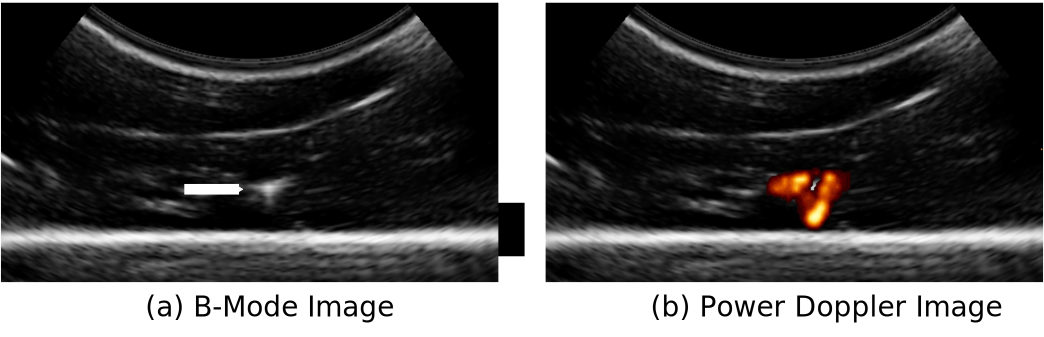
\includegraphics[width=\textwidth]{Images/Chapter2/2DUS/2DUS}%
\caption[2D ultrasound images from 3D sweeps of needle]{2D ultrasound images taken from volumetric sweeps of steerable needles inserted into \textit{ex vivo} liver: (a) B-mode ultrasound image used for manual segmentation. The needle cross section is indicated. (b) Corresponding power Doppler ultrasound image captured during needle vibration. The Doppler response surrounds the needle cross section.}
\label{fig:2DUS}
\end{figure*} 

\label{sec:Results}
Fig.~\ref{fig:2DUS} shows example 2D ultrasound images taken from volumetric sweeps of steerable needles in \textit{ex vivo} liver. Both B-mode and power Doppler images are shown. The needle cross section was visible in approximately 50 percent of the B-mode images captured over most sweeps. As shown in the figure, the high-frequency vibration of the needle causes a power Doppler response centered around the needle cross section.

\begin{figure*}[!t]
\centering
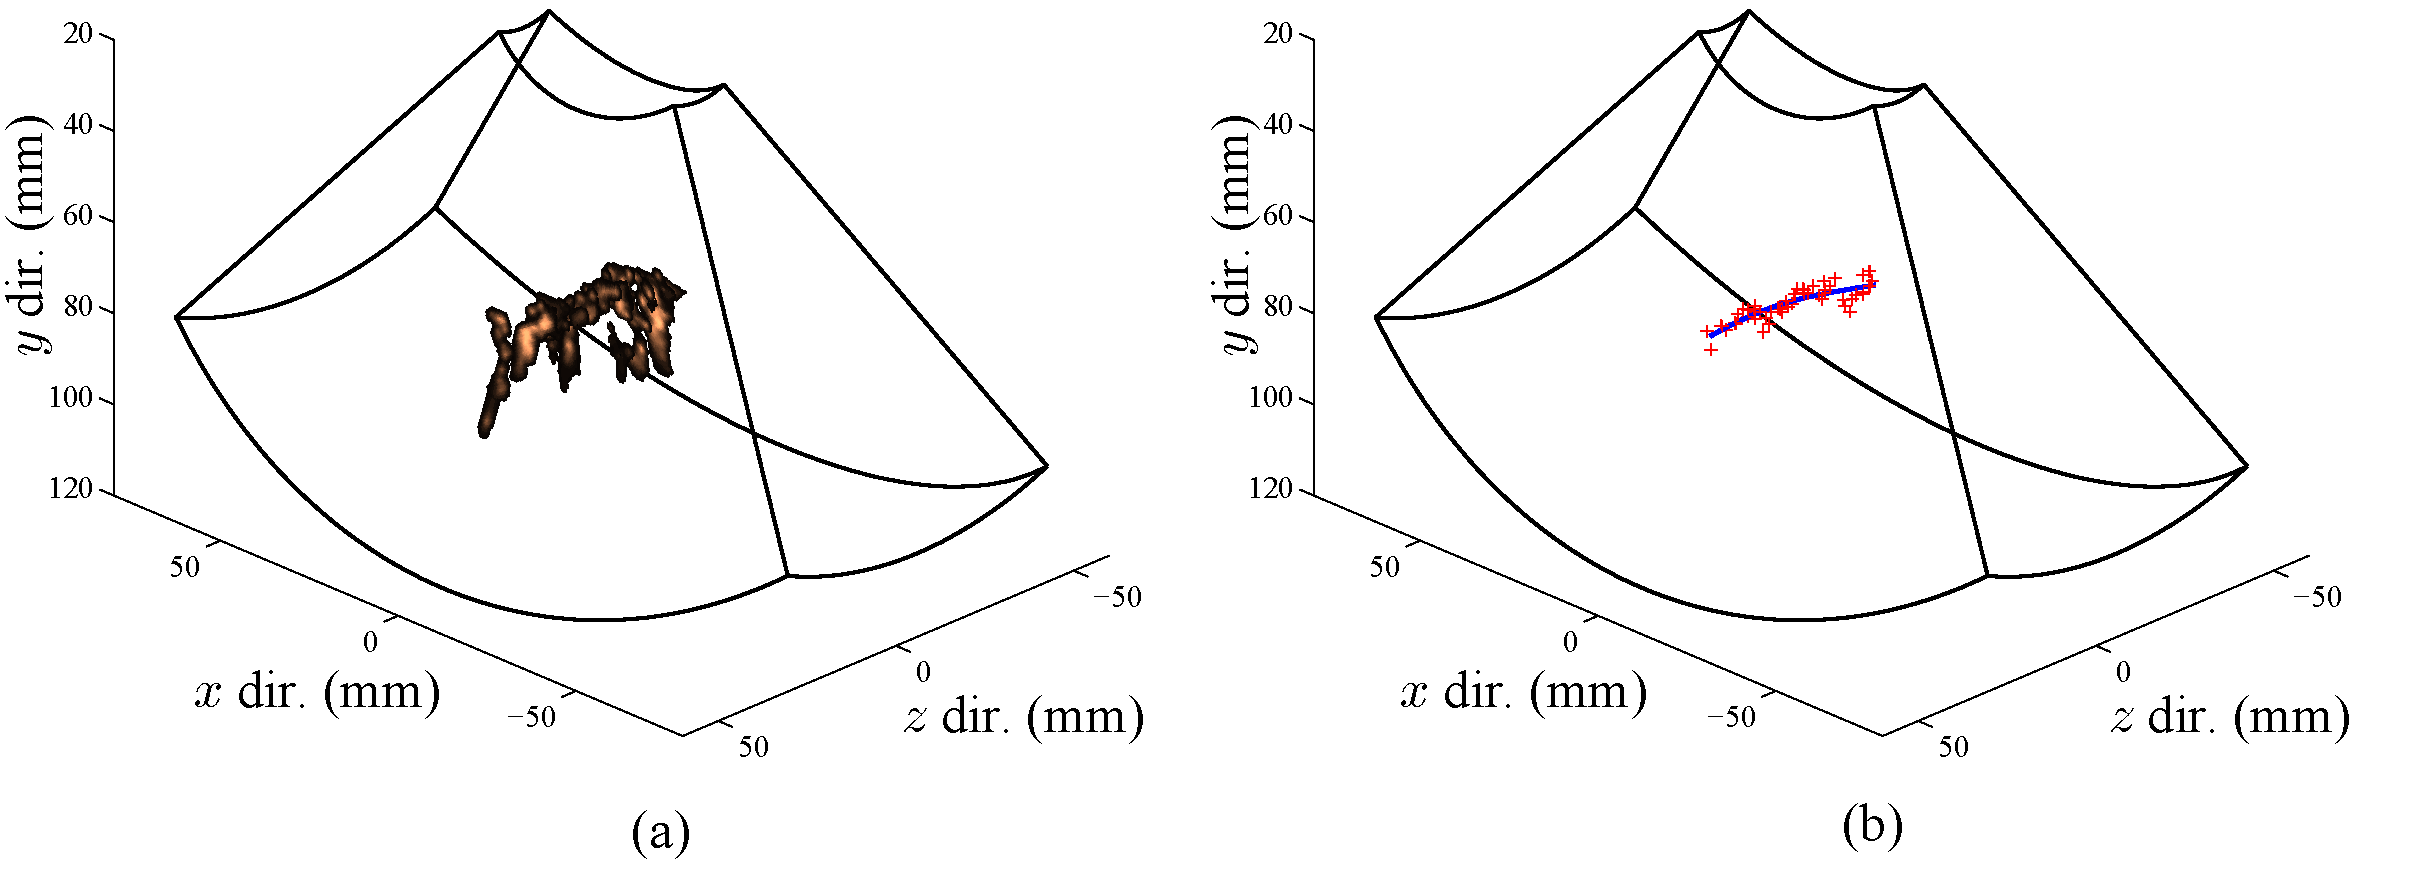
\includegraphics[width=\textwidth]{Images/Chapter2/DopplerVisualization/Doppler3D}%
\caption[Example segmentation of needle using Doppler method]{Example segmentation of needle using Doppler method: (a) Power Doppler response around the needle in each image. (b) Reconstructed needle shape (blue curve), fit through the centroids of the Doppler data in each image (red crosses).}
\label{fig:SegmentationExample}
\end{figure*}   

Fig.~\ref{fig:SegmentationExample} shows the 3D Doppler data generated by a vibrating needle, along with the corresponding Doppler centroids and best-fit polynomial curve. Volumetric framerate using the SonixMDP system was 0.2~Hz for power Doppler data at an imaging depth of 50~mm. Software runtimes were approximately 60~ms per image for the 2D image processing algorithm and 15~ms per sweep for the steering controller, when implemented on the SonixMDP's integrated processor.

\subsection{Segmentation Accuracy}
Fig.~\ref{fig:SegmentationError} summarizes the results of the segmentation accuracy tests. Across all tests, the maximum segmentation error was 3.18~mm, the minimum segmentation error was 0.13~mm, the mean segmentation error was 1.24~mm, and the standard deviation of the segmentation error was 0.57~mm. In the base case tests (straight, 0.48-mm needle centered in the image and vibrated at 600~Hz), the mean segmentation error was 0.92~mm and the standard deviation of the segmentation error was 0.93~mm.

In the needle curvature test, curved and straight needles had similar segmentation errors, with somewhat higher errors in the curved configuration. The mean error was 0.85~mm for straight needles, and 1.36~mm for curved needles. We conclude that for transducers initially oriented as shown in Fig.~\ref{fig:SliceConcept}, our segmentation method is suitable for the range of needle geometries that can be achieved by bent tip steering in biological tissue (assuming $\rho_{\text{min}} \approx$ 50~mm). The implementation described in this chapter fails if the steerable needle is exactly parallel to the imaging plane, thus presenting a linear rather than circular cross section. However, this can be avoided by placing the 3D transducer so the needle is initially approximately perpendicular to the imaging plane. Applying the Doppler segmentation technique without constraint on the transducer orientation, and with other 3D ultrasound implementations---such as freehand tracked 3D ultrasound---is addressed in Chapter 4.

\begin{figure*}[!t]
\centering
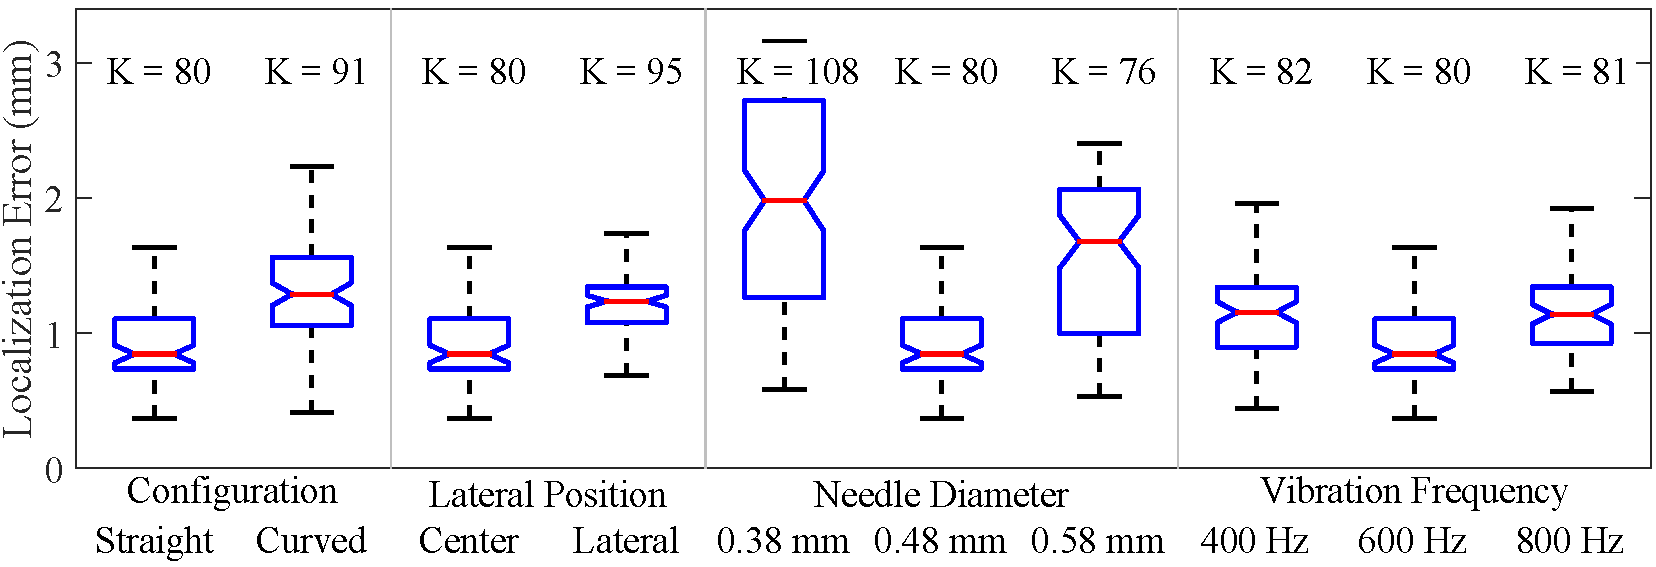
\includegraphics[width=\textwidth]{Images/Chapter2/SegmentationAccuracy/SegmentationAccuracy}%
\caption[Doppler segmentation accuracy results]{Segmentation accuracy results. Two needle configurations (straight, curved), two image positions (center, lateral), three needle diameters (0.38~mm, 0.48~mm, 0.58~mm), and three vibration frequencies (400~Hz, 600~Hz, 800~Hz) were tested. For each group, red line indicates median error, blue box indicates 25th and 75th percentile, and whiskers indicate minimum and maximum error. Number of data points for each group is also indicated.}
\label{fig:SegmentationError}
\end{figure*}

Needle diameter had a significant effect on segmentation accuracy. Mean error was 0.85~mm for 0.48-mm needles, versus 1.98~mm for 0.38-mm needles and 1.68~mm for 0.58-mm needles. The significant change in mean error for the 0.48-mm needles is surprising given the relatively small change in needle diameter. The complexity of the wave mechanics that govern the transmission of vibrations along a flexible needle in viscous tissue makes it difficult to theorize why needle diameter appears to be an important factor. This issue is worthy of future study for two reasons. First, because improved understanding of the motion around the vibrating needle might allow for new Doppler processing algorithms that specifically target the generated motion. Second, because specific needle geometries may be required for other clinical applications (for example, brachytherapy systems would likely require hollow needles).

Lateral image position and vibration frequency did not have significant impacts on segmentation accuracy. In the lateral position test, the mean error was 0.85~mm for needles centered in the image, and 1.24~mm for needles on the lateral edge. In the vibration frequency test, the mean error was 1.16~mm for 400-Hz vibration, 0.85~mm for 600-Hz vibration, and 1.14~mm for 800-Hz vibration. In the case of vibration frequency, the insensitivity is in agreement with our previous study~\cite{Adebar2013}, where varying vibration frequency over a much larger range did not significantly affect segmentation accuracy. 

\subsection{Closed-Loop Steering}
Table~\ref{table:Targeting Results} lists results from six successful closed-loop needle steering tests. For each test, the number of insertion increments ($N_{\text{inc}}$), the $x$-$y$-$z$ dimensions of the complete needle steering path ($\delta x$, $\delta y$, and $\delta z$), and the final error in tip placement relative to the target ($e_{\text{final}}$) are listed. Mean tip placement error was 1.57~mm over the six tests, which is close to the mean error in Fig.~\ref{fig:SegmentationError} for that configuration. 

\begin{figure*}[!t]
\centering
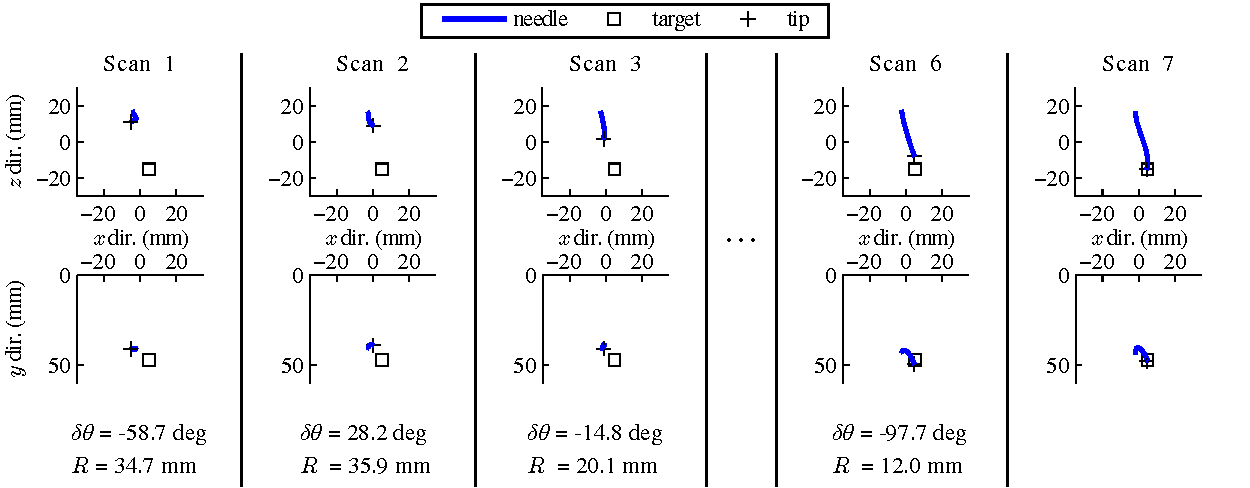
\includegraphics[width = \textwidth]{Images/Chapter2/Steering/Steering}%
\caption[Closed-loop needle steering results]{Closed-loop needle steering results. Orthogonal views of successive incremental scans during needle steering in \textit{ex vivo} tissue, with the output from the steering controller after each scan below. The needle base was inserted 5~mm between each scan, with rotation and duty cycle determined by the steering controller. Error in placing the tip at the target bead was 0.86~mm after the final insertion.}
\label{fig:SucessfulSteering}
\end{figure*}

Fig.~\ref{fig:SucessfulSteering} shows the needle shapes reconstructed during incremental closed-loop steering in Test~6. The $y_{\text{tip}}$-axis was initially aligned with the $y$-axis of the ultrasound coordinate system. After Scan 1, the steering controller compensated by rotating the $y_{\text{tip}}$-axis towards the target ($\delta\theta = -58.7 \text{ degrees}$). The steering controller gave smaller corrections based on Scans 2 to 5, as a result of deviation from the steering model and noise in the measurement of point ${p}$. After Scan 6, when the needle tip was within several millimeters of the target, the steering controller output a large unnecessary rotation correction ($\delta\theta = -97.7 \text{ degrees}$), but over such a small distance it had little effect. Final tip placement error $e_{\text{final}}$ was 0.86~mm for this test.

\begin{table}[!t]
% increase table row spacing, adjust to taste
\renewcommand{\arraystretch}{1.3}
\centering
\caption{Closed-loop needle steering results}
\label{table:DopplerTargetingResults}
% Some packages, such as MDW tools, offer better commands for making tables
% than the plain LaTeX2e tabular which is used here.
\begin{tabulary}{\columnwidth}{| c | C | C | C | C | C |}
\hline
Test & $N_{\text{inc}}$ \newline  & $\delta x$ \newline (mm) & $\delta y$ \newline (mm) & $\delta z$ \newline (mm) & $e_{\text{final}}$\newline (mm)\\
\hline
1 	& 6 &	1.99   &   10.74  &   29.09  &	1.57    \\
\hline
2 	& 7 &	8.42   &   7.15   &   29.16  &	1.73	\\
\hline
3 	& 6 &	7.81   &   2.63   &   31.44  &	1.27	\\
\hline
4 	& 6 &	8.04   &   6.81   &   31.78  &	2.08    \\
\hline
5	& 6 &	1.75   &   5.06   &   26.46  & 	1.89    \\
\hline
6 	& 6 &	6.13   &   3.83   &   32.26  &	0.86    \\
\hline
\end{tabulary}
\end{table}

In addition to the six tests listed in Table~\ref{table:DopplerTargetingResults}, there were several tests which failed as a result of poor needle steering behavior. Bent-tip needle steering requires a homogeneous solid medium. If the steerable needle tip impacts an obstacle which it does not pierce through, such as a bone or blood vessel, the path of the needle may deviate greatly from what is expected. Fig.~\ref{fig:Steering} shows the reconstructed needle shapes from one such failed test. In this test, the needle appeared to impact one of several small vessels that could be visualized in ultrasound before the final scan. Fig.~\ref{fig:LiverVessel} shows examples of these small vessels in a section of liver specimen.

\begin{figure*}[!t]
\centerline{\subfigure[ ]{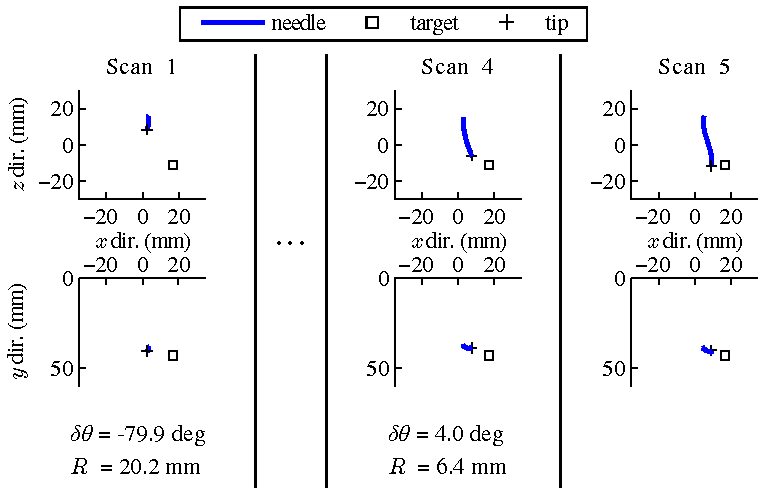
\includegraphics[width = 0.6\textwidth]{Images/Chapter2/FailedSteering/Steering}%
\label{fig:Steering}}
\hfil
\subfigure[ ]{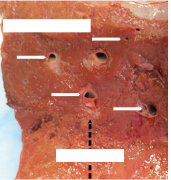
\includegraphics[height=2.2in]{Images/Chapter2/FailedSteering/LiverVessel}%
\label{fig:LiverVessel}}}
\caption[Closed-loop needle steering results; failed steering trial]{Closed-loop needle steering results. Example of failed needle steering: (a) Orthogonal views of successive incremental scans during needle steering in \textit{ex vivo} tissue, with the output from the steering controller after each scan below. The needle base was inserted 5~mm between each scan, with rotational orientation and duty cycle setting determined by the steering controller outputs. Error in placing the tip at the target bead was 8.14~mm after the final insertion. The needle failed to reach the target due to interference from internal vessels that could  be visualized in the ultrasound images. (b) Section of tissue sample with example vessels and approximate direction of needle insertion indicated.}
\label{fig:FailedSteering}
\end{figure*}

\subsection{Discussion}
The methods described in this chapter are capable of segmenting a curved needle with average error of 1 to 2~mm, and steering a needle to a target with an average error of 1.57~mm. This is roughly equivalent to manual targeting error with medical image guidance, which has been shown to be 2~mm or higher on average~\cite{Crocetti2008,MaierHein2008,Schubert2013}. Studies of percutaneous RFA of liver cancer generally suggest that an ablative margin of 5-10~mm around a tumor is necessary to prevent recurrence of cancer~\cite{Dodd2001,Kim2006,Gervais2009}. However recent work has reported that ablative margins as small as 3~mm are associated with a lower rate of local tumor progression~\cite{Kim2010}. This suggests that a targeting error of 2~mm may be tolerable. Overall, the experimental results described in this chapter show that our segmentation and control algorithms approach the accuracy and consistency necessary for a practical clinical application such as RFA of liver cancer. 

In this chapter, we applied our segmentation and control algorithms to sequences of incremental insertions, rather than to constant velocity insertions. We believe this is the most realistic approach in a clinical setting. Although a delay of several seconds for ultrasound scanning after each incremental insertion might seem undesirable to roboticists, it actually mirrors current clinical practice where clinicians frequently pause during needle insertion to take CT scans. 

Needle vibration in this chapter is achieved by an actuator connected to the proximal end of the steerable needle. In this implementation, the Doppler response decreases moving along the needle towards the tip, as the vibrations are damped out by the surrounding tissue. For very long insertion paths, or more viscous tissues, the amplitude of vibration at the tip might be too small to allow a reliable Doppler segmentation. We are currently exploring other actuation schemes that vibrate the needle tip directly, as in~\cite{Harmat2006} or~\cite{McAleavey2003}, although integrating these actuators into sub-millimeter steerable needles is a difficult practical problem.

With vibration of the needle, the added potential for tissue damage is an issue that must be considered carefully. Unfortunately, both the tissue strain around the vibrating shaft and the displacement of the sharp needle tip are difficult to measure experimentally, and it was not possible to quantify these factors in the current work. Histological analysis after steering in an \textit{in vivo} model, as in~\cite{Majewicz2012}, would likely be required to evaluate tissue damage. As stated above, the displacement of the needle shaft is in the sub-millimeter range at the needle base, and decreases along the needle shaft due to tissue damping. While we thus expect the resulting tissue damage to be minimal, this issue is again worthy of further study.

It should be noted that the duty cycling approach we apply to control steerable needle curvature has largely been validated in homogeneous artificial tissues, although several examples of duty cycling in biological tissues have been reported~\cite{Swaney2013,Engh2010,Patil2014}. Recent work~\cite{Patil2014} suggests that the linear relationship between duty cycle and curvature described in Equation (\ref{eq:DC}) may oversimplify steerable needle behavior in heterogeneous biological tissue. Fortunately the closed-loop structure of our steering algorithm compensates for deviation from the expected relationship, and for variation in $\rho_\text{min}$.
%!TEX root = PhD_Thesis.tex
\chapter[Improving Needle Curvature]{Improving the Curvature of Steerable Needles in Biological Tissue}

\section{Introduction}
This chapter describes methods for improving the curvature of steerable needles in liver tissue. This work was motivated by our early benchtop and cadaver testing, where we found that steerable needles did not follow as tightly curved paths in \textit{ex vivo} liver tissue as in artificial tissues such as PVC. 

A survey of the needle steering literature shows that experimental validation of the different needle steering techniques has been performed in artificial tissue simulants~\cite{DiMaio2005,Mallapragada2009,Okazawa2005,Ko2013,Patil2014,Swaney2013,Ayvali2012,Datla2014,Ryu2014,Rucker2013,vandeBerg2015}, \textit{ex vivo} biological tissue samples~\cite{Glozman2007,Burdette2010,Patil2014,Swaney2013,Majewicz2012,Rucker2013}, and in one live canine model~\cite{Majewicz2012}. Compared to other needle steering techniques~\cite{DiMaio2005,Mallapragada2009,Okazawa2005,Ko2013,Ryu2014}, bent-tip steerable needles have shown the most promising performance results (i.e., have followed the most tightly curved paths) in both artificial tissue simulants and biological tissues. Bent-tip steerable needles generally perform better in artificial tissue simulants than in biological tissues, presumably because artificial tissue simulants are stiffer and more homogeneous. Experimental studies testing bent-tip steerable needles in artificial tissue simulants have reported radius-of-curvature values of 67~mm~\cite{Patil2014}, 121~mm~\cite{Swaney2013}, and 128~mm~\cite{Rucker2013}. Experimental studies testing bent-tip steerable needles in \textit{ex vivo} biological tissues have reported radius-of-curvature values of 41.7~mm~\cite{Majewicz2010}, 51.4~mm~\cite{Adebar2014}, 137~mm~\cite{Patil2014}, 176~mm~\cite{Swaney2013}, 200~mm~\cite{Majewicz2012}, and 400~mm~\cite{Rucker2013}. In the only reported \textit{in vivo} test, bent-tip steerable needles followed curved paths with radii of curvature from 104~mm to 143~mm in canine kidney and liver tissue~\cite{Majewicz2012}.

The requirement for needle curvature is specific to the clinical application under consideration. It depends on the geometry of the target anatomy, and the desired use case for needle steering; in other words, whether needle steering will be used to correct for small errors in straight-line targeting, or to reach widely divergent targets or targets obscured by obstacles. Although existing techniques may be useful for small error corrections, our goal is to use needle steering in percutaneous RFA of liver tumors to reach multiple targets throughout the liver from a single wound to the liver capsule, thus reducing the risk of hemorrhage, and to reach targets high in the liver dome and targets blocked by large-diameter vasculature, thus treating patients who would otherwise be excluded. Based on the curvature results reported to date, it was reasonable to question whether existing steerable needles are capable of creating curved needle paths in biological tissues that are clinically relevant to our application.

This chapter is divided into three main sections. In Section~\ref{sec:workspaceAnalysis}, we describe a workspace analysis of medical image data, intended to set a procedure-specific requirement for needle curvature in ablation of liver tumors. This work was previously published in the proceedings of the 2014 Hamlyn Symposium on Medical Robotics~\cite{Adebar2015}. In Section~\ref{sec:TipGeometryAnalysis}, we describe finite-element (FE) modeling and experimental testing undertaken to improve understanding of needle-tissue interaction during bent-tip needle steering. In Section~\ref{sec:Articulated-TipNeedle}, we describe the design and validation of a new articulated-tip steerable needle, which uses changes in tip geometry, as suggested by the results of Section~\ref{sec:TipGeometryAnalysis}, to achieve tighter curvature in liver tissue than any comparable technique. The work described in Section~\ref{sec:workspaceAnalysis} and  Section~\ref{sec:TipGeometryAnalysis} was previously published in the IEEE Transactions on Biomedical Engineering~\cite{Adebar2015a}.

\section{Procedure-Specific Workspace Analysis}
\label{sec:workspaceAnalysis}
\subsection{Methods}
An open-source contrast-enhanced abdominal CT scan of a healthy 36-year-old male was analyzed~\cite{Pieper2004}. The segmented liver capsule was exported from 3D Slicer, refined using Meshlab, and imported into Matlab to serve as a workspace boundary. Similarly, large-diameter portions of the internal vasculature which represent a significant bleeding risk (specifically the hepatic and portal veins with diameter over approximately 5 mm) were imported to serve as obstacles. These models are shown in Fig.~\ref{fig:Meshes3D}. 

\begin{figure*}[!t]
\centering
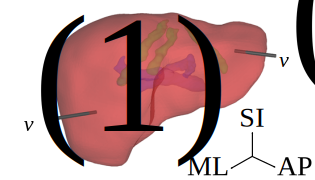
\includegraphics[width = 0.75\textwidth]{Images/Chapter3/Meshes3D/Meshes3D}%
\caption[Models of the liver anatomy]{Models of the liver boundary (capsule), large hepatic veins (green) and large portal veins (blue). The entry vectors are also indicated. The superior-inferior (SI), medial-lateral (ML), and anterior-posterior (AP) directions are shown.}
\label{fig:Meshes3D}
\end{figure*}

Two entry vectors $v^{(i)}$ were defined based on typical introducer placement for percutaneous RFA of liver tumors. Vector $v^{(1)}$ represents an intercostal approach into the right liver. Vector $v^{(2)}$ represents an anterior subcostal approach under the costal margin into the left liver. Both orientations reflect insertion under ultrasound guidance with the needle at 45 degrees to the transducer axis. 

For each $v^{(i)}$, the corresponding reachable workspace $R^{(i)}$ was measured by discretizing the liver volume $L$ (excluding the vasculature) into 4-mm voxels, and determining if each voxel could be reached by a permissible path. Paths that crossed the liver boundary (capsule) or vasculature were excluded to decrease risk of bleeding and other complications. Paths were also restricted to have one or two constant-curvature sections. Although insertion and rotation of a bent-tip steerable needle can theoretically generate more complex needle paths, in practice the mechanical properties of liver cause these complicated paths to relax into simpler paths. Two-section paths were excluded if the waypoint was already beyond the target (i.e., if the dot product of the vector from the waypoint to the target and the tangent vector at the waypoint was negative) to avoid impractical looping behavior. Finally, paths were excluded if they required radius of curvature $\rho$ below threshold $\rho_{\text{min}}$, which was varied as a parameter from 10-200~mm. Fig.~\ref{fig:Paths} shows examples of permissible and excluded paths. 

\subsection{Results}
\begin{figure*}[!t]
\centering
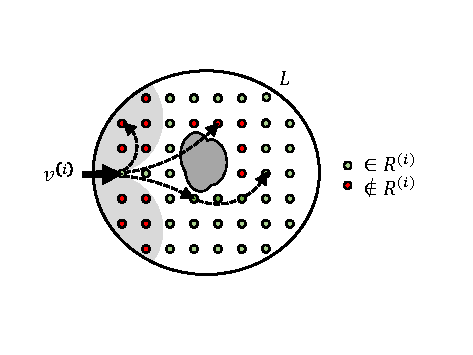
\includegraphics[width = 0.6\textwidth]{Images/Chapter3/Paths/Paths}%
\caption[Excluded and permissible paths]{Reachable and unreachable voxels within $L$, and lines showing, from left to right, an excluded path that violates $\rho_{\text{min}}$, an excluded path that passes through an obstacle, and a permissible two-part path. }
\label{fig:Paths}
\end{figure*}

Fig.~\ref{fig:ReachableSizeByRho} shows the size of the reachable set---specified by the ratio of the set sizes $\lvert R^{(i)} \rvert / \lvert L \rvert$---as a function of minimum radius of curvature $\rho_{\text{min}}$. With $\rho_{\text{min}} =$ 100~mm, paths starting at $v^{(1)}$ were able to reach approximately 8 percent of $L$, while paths starting at $v^{(2)}$ were able to reach approximately 41 percent of $L$. 

\begin{figure*}[!t]
\centering
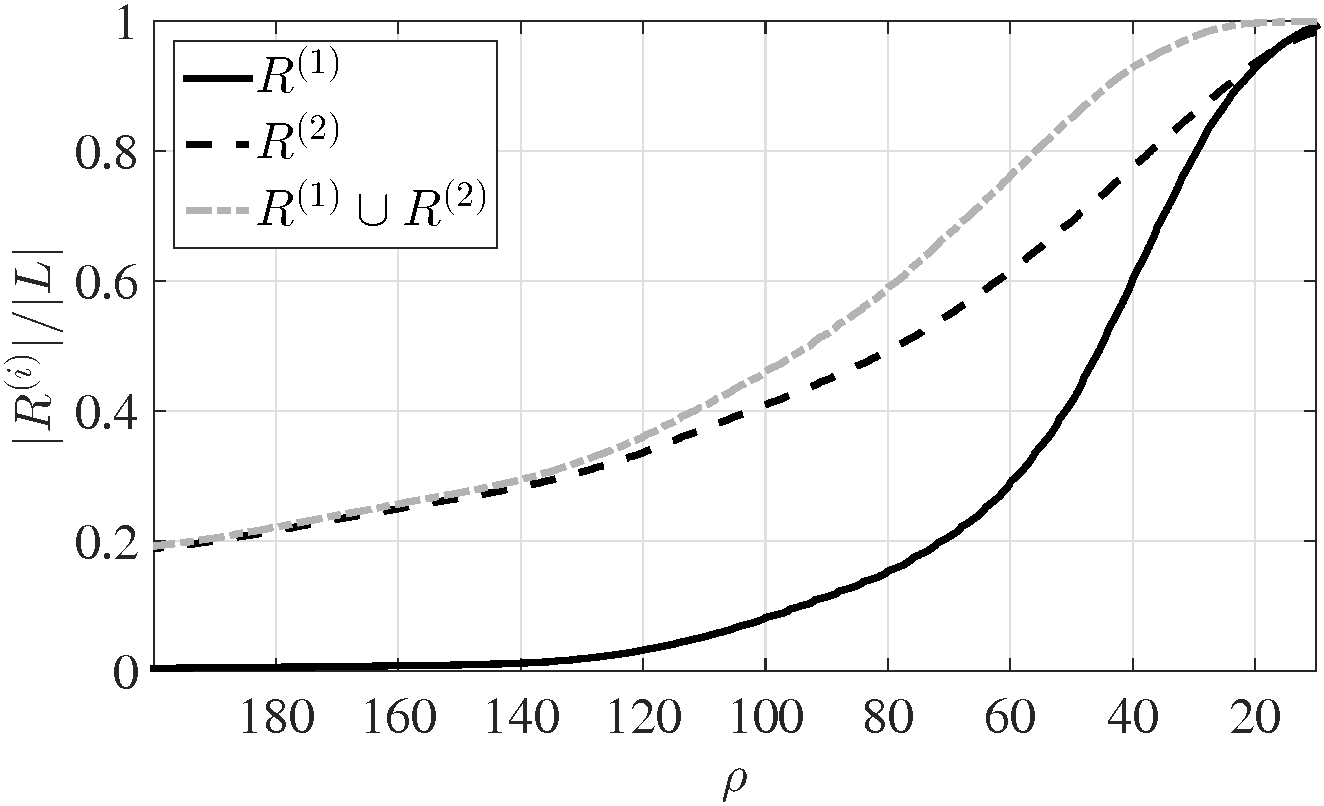
\includegraphics[width = 0.7\textwidth]{Images/Chapter3/ReachableSizeByRho/ReachableSizeByRho}%
\caption[Reachable set size as a function of $\rho_{\text{min}}$]{Ratio of reachable set size to total liver size as a function of minimum radius of curvature $\rho_{\text{min}}$. Results for intercostal ($v^{(1)}$) and anterior approaches ($v^{(2)}$) are shown.}
\label{fig:ReachableSizeByRho}
\end{figure*}

Fig.~\ref{fig:ReachableSizeByRho} shows a frontal slice near the center of the liver, with color indicating radius of curvature $\rho$ required to reach each voxel from $v^{(1)}$. The needle was not able to reach areas behind the hepatic veins and surrounding the insertion. Most of the slice was reachable using single-section paths, except for the area blocked by the vessels.

\subsection{Discussion}
Results shown in Fig.~\ref{fig:ReachableSizeByRho} reveal the gap between current needle steering methods and our clinical application. Most steerable needle curvatures $\rho_{\text{min}}$ reported in biological tissue are between 100-200 mm [2]. Even combining the intercostal and anterior subcostal approaches, such needles would only permit access to 50 percent of the liver at best. Since the distribution of tumor sites is approximately uniform throughout the liver, current steerable needles would be unable to access many targets. Although angling the introducer could change the results shown in Fig. 4, interference from the ribs and potential for tissue injury limit this degree of freedom after initial insertion. 

An important potential advantage of needle steering in RFA of liver tumors is the ability to reach targets in the dome of the liver (on the right-lateral superior surface), which can be very difficult in some patients using traditional RFA probes due to interference from the ribs. As seen in Fig.~\ref{fig:FrontalSlice}, a radius of curvature of approximately 50~mm is necessary to reach the right-lateral aspect of the liver dome. We believe $\rho_{\text{min}} = 50$~mm is thus a reasonable curvature requirement for future development, since it allows the needle to access the liver dome, and reach approximately 85 percent of the liver volume from the entry points we have described.
  
\begin{figure*}[!t]
\centering
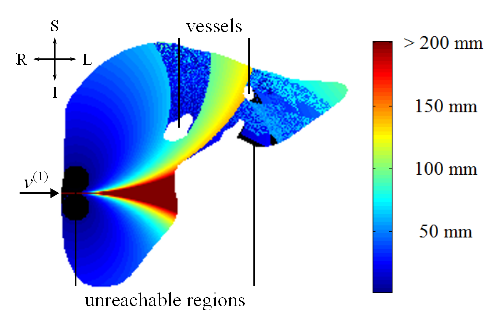
\includegraphics[width = 0.6\textwidth]{Images/Chapter3/FrontalSlice/FrontalSlice}%
\caption[Visualization of reachable set size]{Frontal slice of $L$. Colors indicate the radius of curvature $\rho$ required to reach each voxel. Black voxels were not reachable with any curvature in the examined range (10-200~mm). White voxels, including vessels inside the liver, were outside $L$.}
\label{fig:FrontalSlice}
\end{figure*}  

%-------------------------------------------------------------------------
\section{Analysis of Tip Geometry }
%-------------------------------------------------------------------------
\label{sec:TipGeometryAnalysis}
\begin{figure}[!t]
\centering
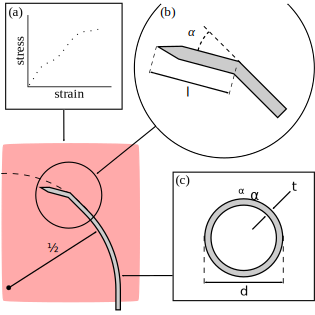
\includegraphics[width = 0.6\columnwidth]{Images/Chapter3/CurvatureFactors/CurvatureFactors}%
\caption[Factors impacting steerable needle curvature]{Factors impacting the radius of curvature $\rho$ of bent-tip steerable needles in liver tissue include (a) mechanical properties of the tissue (modeled as a hyperelastic solid), (b) tip geometry (defined by length $l$ and angle $\alpha$), and (c) needle material and cross section (defined by diameter $d$ and wall thickness $t$). In this chapter, we exclusively consider the impact of tip length $l$ and tip angle $\alpha$.}
\label{fig:NSFactors}
\end{figure}
As shown in Fig.~\ref{fig:NSFactors}, several factors impact the radius of curvature of steerable needles in tissue. In this dissertation we focus exclusively on the geometry of the bent tip. Bent-tip steerable needles described to date have generally had tip length $l \approx$~4~mm, and tip angle $\alpha \approx$~30~degrees~\cite{Patil2014,Swaney2013,Rucker2013,Majewicz2012}. Since bent-tip needles steer as a result of the asymmetric lateral force at the tip, it is reasonable to expect that a greater asymmetry---i.e., larger tip length $l$ or tip angle $\alpha$ as shown in Fig.~\ref{fig:NSFactors}---would result in improved curvature. However, because of the complex mechanics of needle-tissue interaction, it was unclear how altering tip parameters over a larger range of values than previously considered~\cite{Majewicz2010} would affect curvature performance. The work described in this section was meant to improve our understanding of the relationship between bent-tip geometry and radius of curvature. We proceeded in two ways. First, we used a simplified FE model of a bent tip moving in tissue to gain insight into the general relationship between tip length, tip angle, and steerable needle curvature. Second, we performed experimental testing to measure the actual needle radius of curvature $\rho$ achieved by bent-tip needles with different geometries in liver tissue.

Although some radius-of-curvature values in \textit{ex vivo} liver tissue have been reported close to or below our 50-mm requirement (our results in Chapter 3, and in ~\cite{Majewicz2010}), the needles in these tests were solid Nitinol wires approximately 0.5~mm in diameter. These solid wires would be unable to deliver payloads such as contrast fluid, ethyl alcohol, or ablation leads. As we work towards early-stage clinical tests in the liver, steerable needle design requirements are increasingly driven by practical issues, such as the need to deliver a payload, or the need to pass through a rigid introducer sheath accessing the liver itself through layers of skin and fat.

\subsection{Finite-Element Model}
The physical interactions between a flexible steerable needle and soft tissue during insertion are extremely complex and difficult to approximate. In prior work, analytical methods~\cite{Misra2010} and FE models with cohesive elements~\cite{Misra2008} were used in an attempt to quantify tip forces and the resulting radius of curvature for bevel-tip steerable needles. Rather than create a more complicated model that encapsulates a bent-tip needle, in our current FE work, the goal was to use a simplified model to gain qualitative insight into the impact of the two specific parameters, bent-tip length and angle, on radius of curvature. As suggested in~\cite{Mahvash2001,Misra2010,Barbe2007}, continuous steerable needle insertion can be considered as a repeated discretized sequence of two steps. In the first step, the needle is inserted and deforms the tissue, resulting in forces at the needle tip and along the needle shaft. In the second step, the tissue ruptures. To make the FE modeling more tractable, we eliminated tissue rupture from the model, and only considered tissue loading. 

\begin{figure*}[!t]
\centering
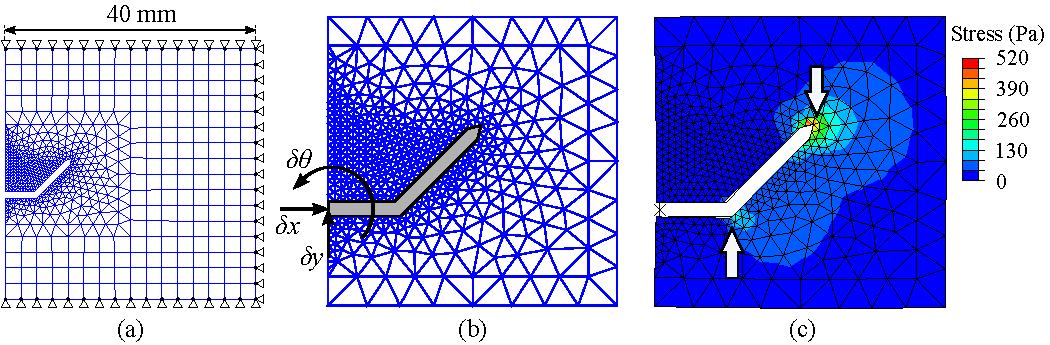
\includegraphics[width = \textwidth]{Images/Chapter3/Abaqus/Abaqus}%
\caption[Planar finite-element model of needle-tissue interaction]{Planar finite-element model of needle-tissue interaction: (a) The tissue was modeled as a square specimen with side length of 40~mm, with complete 3DOF constraints on three sides. A coarse quadrilateral mesh was used for most of the tissue, with a finer triangular mesh in the neighborhood of the needle tip. The needle tip was modeled as a rigid body, while the tissue was modeled as an incompressible hyperelastic solid. (b) The input to the model was horizontal displacement $\delta x$ of the needle. The output from the model was the rotation of the needle $\delta\theta$ and vertical displacement $\delta y$. These were used to calculate radius of curvature $\rho$. (c) After insertion, stress developed in the tissue, and was highest near the tip of the needle.}
\label{fig:Abaqus}
\end{figure*}

\begin{figure}[!t]
\centering
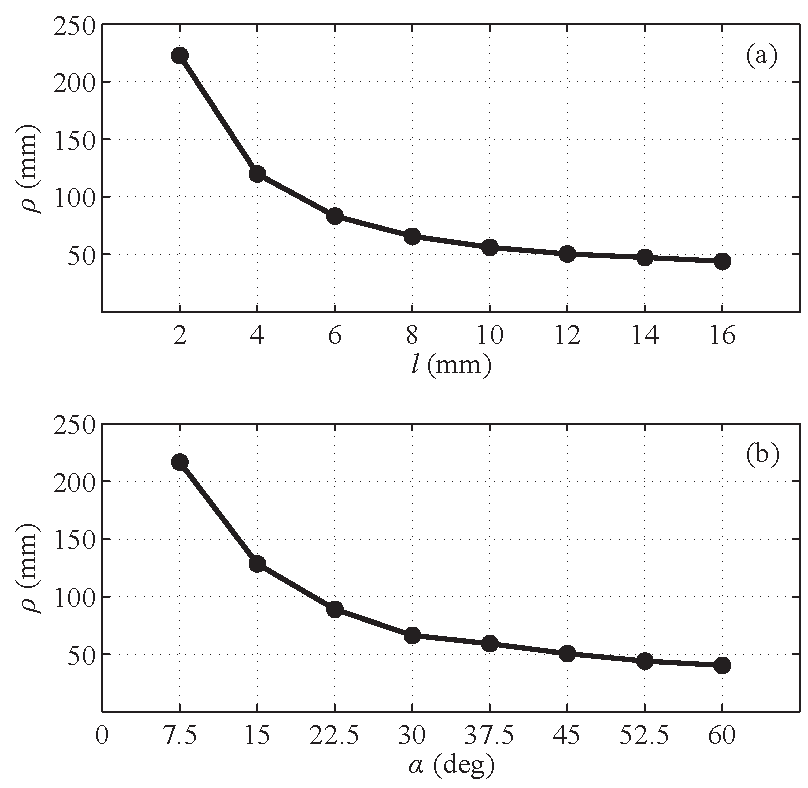
\includegraphics[width=0.6\columnwidth]{Images/Chapter3/AbaqusResults/AbaqusResults}%
\caption[Finite-element simulation results]{Finite-element simulation results: (a) Impact of bent-tip length $l$ on simulated radius of curvature $\rho$. (b) Impact of bent-tip angle $\alpha$ on simulated radius of curvature $\rho$.}
\label{fig:AbaqusResults}
\end{figure}

A 2D FE simulation was created using Abaqus Standard (Dassault Systemes; Velizy Villacoublay, France) with a static analysis step. The tissue was modeled as an incompressible hyperelastic solid, with Mooney-Rivlin coefficients as measured in~\cite{Kim2005}. A 40-mm square tissue specimen was modeled with its boundaries fully constrained on three sides, and free on the insertion face. The tissue was meshed with coarse quadrilateral elements (CPE4H), and finer triangular elements (CPE3H) in the contact region, as shown in Fig.~\ref{fig:Abaqus}. A mesh convergence test ensured the element size was sufficiently fine. Contact between the needle and tissue was modeled as frictionless as in~\cite{Misra2008}. Since bent-tip needles are generally created with inflexible steel or brass tips, the bent tip (including the distal 5~mm of the needle shaft) was modeled as a rigid body. The needle tip was free to translate in the $y$ direction and rotate. A linear torsional spring interaction was applied to the base of the rigid body, in order to model the needle shaft's resistance to bending. The spring constant was selected to yield $\rho = 120$~mm for a tip with $l = 4$~mm and $\alpha = 45$~degrees, since this radius of curvature is consistent with values described for similar steerable needle designs in the literature~\cite{Patil2014}, and with our experimental results as described below. The input to the simulation was the horizontal displacement of the needle tip $\delta x$, which was increased from 0.0~mm to 0.5~mm in a uniform ramp. The output of the simulation was the final vertical displacement $\delta y$ and rotation $\delta\theta$ of the bent tip after insertion. The radius of curvature $\rho$ was calculated by chaining together the $\delta x$, $\delta y$ and $\delta\theta$ displacement values obtained from the simulation, and fitting a circle to the resulting points.

\subsection{Finite-Element Results}
Fig.~\ref{fig:Abaqus}(c) shows an example of the FE model at the final simulation increment, with the resulting von Mises stresses in the simulated tissue overlaid on the deformed mesh. The largest stresses were seen around the tip of the needle, suggesting where tissue rupture might occur. Fig.~\ref{fig:AbaqusResults} summarizes FE results, with radius of curvature $\rho$ shown as a function of tip length $l$ and tip angle $\alpha$. Increases in both $l$ and $\alpha$ consistently resulted in reduced $\rho$, although only small reductions resulted beyond $l \approx 10$ mm and $\alpha \approx 45$~degrees.  

\begin{figure}[!t]
\centering
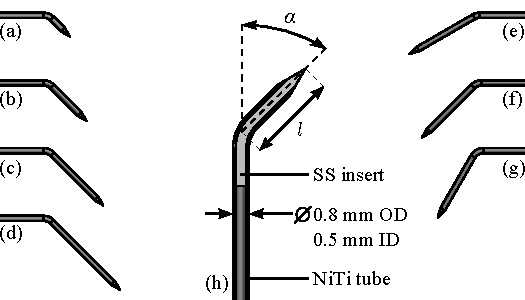
\includegraphics[width=0.65\columnwidth]{Images/Chapter3/Bent-TipGeometry/Bent-TipGeometry}%
\caption[Geometry of bent-tip steerable needles used for testing]{Geometry of bent-tip steerable needles used for testing in \textit{ex vivo} tissue. In the tip-length test, four needles with tip angle of 45 degrees and tip length of (a) 4~mm, (b) 8~mm, (c) 12~mm, and (d) 16~mm were tested. In the tip-angle test, three needles with tip length of 12~mm and tip angle of (e) 30~degrees, (f) 45~degrees, and (g) 60~degrees were tested. A schematic view (h) shows the construction of the bent-tip steerable needles. A Nitinol (NiTi) tube with outer diameter (OD) of 0.8~mm and inner diameter (ID) of 0.5~mm forms the shaft of each needle. A stainless-steel (SS) insert is bonded inside the tube with epoxy to form the tip. The tip is then ground into a cone using an abrasive wheel, and the tip is bent to the appropriate length and angle.}
\label{fig:Bent-TipGeometry}
\end{figure}

\subsection{Testing in \textit{Ex Vivo} Tissue}
In addition to FE simulations, we performed experimental tests in \textit{ex vivo} porcine liver tissue. We measured the impact of tip length $l$ and tip angle $\alpha$ by creating a number of steerable needles and separately varying those two parameters over a range of values. We inserted each needle into a tissue specimen, and measured the radius of curvature $\rho$ of the resulting needle path.

\subsubsection{Bent-Tip Needles}
Four steerable needles with tip angles $\alpha$ of 45~degrees and tip lengths $l$ of 4~mm, 8~mm, 12~mm, and 16~mm were created to test the impact of tip length. Three steerable needles with tip length $l$ of 12 mm and tip angle $\alpha$ of 30~degrees, 45~degrees, and 60~degrees were created to test the impact of tip angle. All the needles were created from Nitinol tubing with an outer diameter of 0.8~mm and an inner diameter of 0.5 mm, as shown in Fig.~\ref{fig:Bent-TipGeometry}.

\subsubsection{Insertion Protocol}
\textit{Ex vivo} porcine liver tissue obtained fresh from a local butcher was used to simulate human liver tissue. Each of the needles described above was inserted into a tissue specimen ten times, using the two-degree-of-freedom robot described in~\cite{Adebar2014}. The needles were inserted with constant velocity along minimum-radius-of-curvature paths; that is, they were inserted without any axial rotation so that the bent tip caused the needle to curve in a single direction. The insertion velocity was approximately 1.6 mm/s. A small incision in the capsule of the liver was used to introduce the needles, since the bent tips were too large for any available introducer sheath. The needles were inserted for a path length of approximately 100 mm, or until the tip of the needle exited the liver. 

\subsubsection{Ultrasound Imaging}
After insertion stopped, the needles were scanned using freehand 3D ultrasound imaging. A SonixMDP ultrasound system (Ultrasonix Research Corp.; Richmond, Canada) with a linear transducer was used to image the needle. This system includes a calibrated electromagnetic tracking system, which enables the collection of 3D ultrasound data. The imaging arrangement was exactly as described in~\cite{Greer2014}. To measure radius of curvature, the needle was segmented from the 3D ultrasound data by manually localizing the needle cross section in the 50 to 150 image frames captured from each insertion. In previous work~\cite{Adebar2014}, we found this manual segmentation to be repeatable to within approximately 0.5~mm. The radius of curvature of the needle was measured by reducing the segmentation points to two dimensions using singular value decomposition, identifying the circular arc that best fit the 2D segmentation points in the least-squares sense, and determining the radius of the arc. The steerable needle's path was generally very close to lying in a plane; across all tests the average distance of the 3D segmentation points from the reduced 2D points was approximately 0.3 mm.

\begin{figure}[!t]
\centering
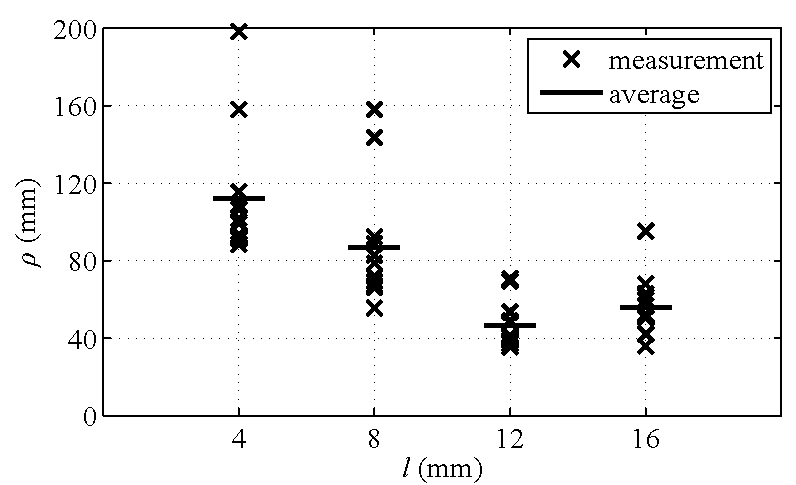
\includegraphics[width=0.6\columnwidth]{Images/Chapter3/CurvatureVsLength/CurvatureVsLength}%
\caption[Impact of bent-tip length $l$ on needle radius of curvature $\rho$]{Summary of experimental results showing impact of bent-tip length $l$ on needle radius of curvature $\rho$ in \textit{ex vivo} tissue. Four tip lengths (4 mm, 8 mm, 12 mm, and 16 mm) were tested. All measured values of $\rho$ are shown, along with average values $\rho_{\text{avg}}$ for each value of $l$.}
\label{fig:CurvatureVsLength}
\end{figure}

\begin{figure}[!t]
\centering
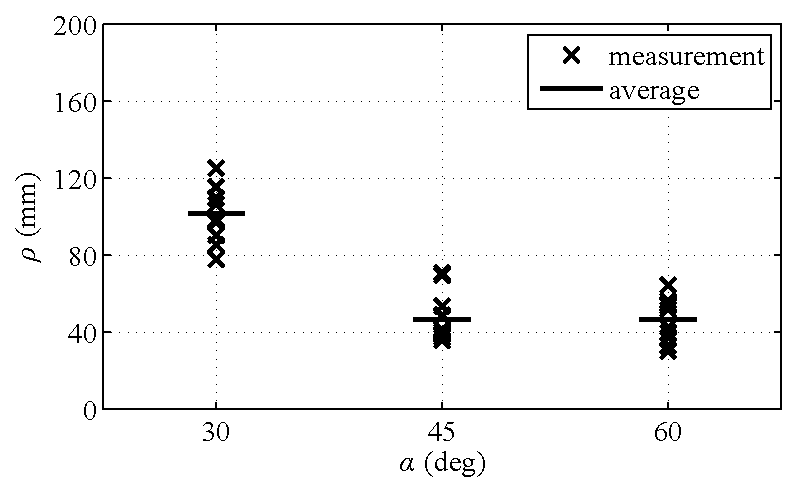
\includegraphics[width=0.6\columnwidth]{Images/Chapter3/CurvatureVsAngle/CurvatureVsAngle}%
\caption[Impact of bent-tip angle $\alpha$ on needle radius of curvature $\rho$]{Summary of experimental results showing impact of bent-tip angle $\alpha$ on needle radius of curvature $\rho$ in \textit{ex vivo} liver tissue. Three tip angles (30 degrees, 45 degrees, and 60 degrees) were tested. All measured values of $\rho$ are shown, along with average values $\rho_{\text{avg}}$ for each value of $\alpha$.}
\label{fig:CurvatureVsAngle}
\end{figure} 

\subsection{Results in \textit{Ex Vivo} Tissue}
Fig.~\ref{fig:CurvatureVsLength} summarizes the measured radius-of-curvature values as a function of the tip length. Average radius of curvature $\rho_{\text{avg}}$ (mean~$\pm$~standard deviation) for $l =$~4~mm, 8~mm, 12~mm and 16~mm was 112.1~$\pm$~33.0~mm, 86.8~$\pm$~31.8~mm, 46.8~$\pm$~12.2~mm and 55.8~$\pm$~15.4~mm respectively. Tip length $l$ of 12 mm resulted in the smallest average radius of curvature, as well as the least variability in curvature. 

Fig.~\ref{fig:CurvatureVsAngle} summarizes the measured radius-of-curvature values as a function of the tip angle. Average radius of curvature $\rho_{\text{avg}}$ (mean~$\pm$~standard deviation) for $\alpha =$~30~degrees, 45~degrees and 60~degrees was 101.4~$\pm$~13.6~mm, 46.8~$\pm$~12.2~mm, and 46.7~mm~$\pm$~10.7~mm respectively. Tip angle $\alpha$ of 60 degrees resulted in the smallest average radius of curvature, although there was substantial variability. Tip angle $\alpha$ of 45 degrees resulted in slightly higher average radius of curvature, but with much less variability.

Fig.~\ref{fig:CurvatureVsLengthData} shows the segmentation results and best-fit circular arcs from the tip-length test. Fig.~\ref{fig:CurvatureVsAngleData} shows the segmentation results and best-fit circular arcs from the tip-angle test.  

\begin{figure*}[!t]
\centering
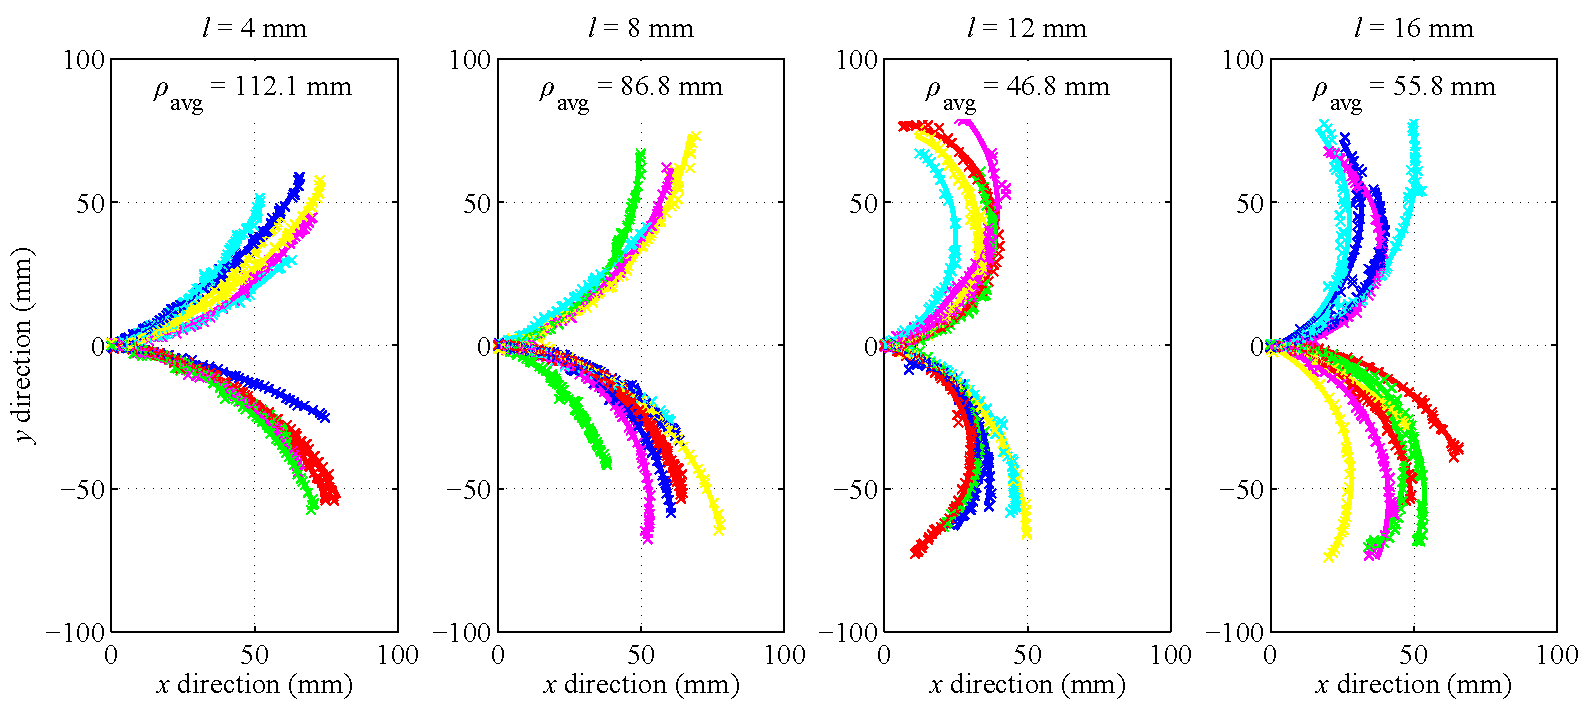
\includegraphics[width=\textwidth]{Images/Chapter3/CurvatureVsLength/CurvatureVsLengthData}%
\caption[Experimental results showing impact of bent-tip length $l$]{Experimental results showing impact of bent-tip length $l$ on needle radius of curvature $\rho$ in \textit{ex vivo} tissue. Four tip lengths (4 mm, 8 mm, 12 mm, and 16 mm) were tested. All segmentation results and average values $\rho_{\text{avg}}$ for each value of $l$ are shown. The needle paths have been moved to a common origin for comparison.}
\label{fig:CurvatureVsLengthData}
\end{figure*}

\begin{figure*}[!ht]
\centering
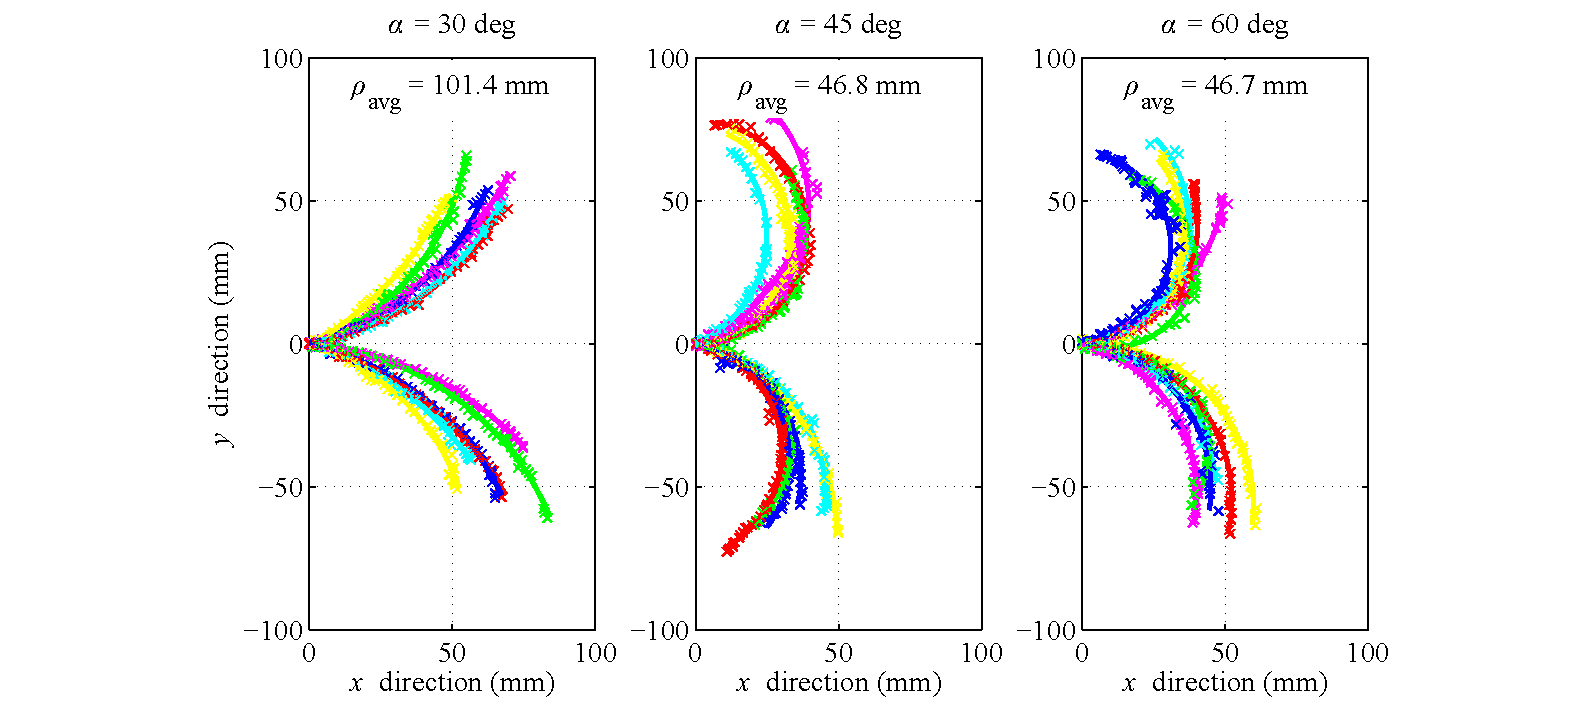
\includegraphics[width=\textwidth]{Images/Chapter3/CurvatureVsAngle/CurvatureVsAngleData}%
\caption[Experimental results showing impact of bent-tip angle $\alpha$]{Experimental results showing impact of bent-tip angle $\alpha$ on needle radius of curvature $\rho$ in \textit{ex vivo} liver tissue. Three tip angles (30 degrees, 45 degrees, and 60 degrees) were tested. All segmentation results and average values $\rho_{\text{avg}}$ for each value of $\alpha$ are shown. The needle paths have been moved to a common origin for comparison.}
\label{fig:CurvatureVsAngleData}
\end{figure*}

\subsection{Discussion}
In the \textit{ex vivo} tip-length test, the needle with $l =$~4~mm and $\alpha =$~45~degrees showed similar radius-of-curvature values to those previously reported using equivalent bent-tip steerable needles in liver tissue~\cite{Patil2014,Swaney2013}. This is expected, since the needles used in those tests had similar tip and shaft geometries to our needles. The needles with $l =$~4~mm and $l =$~8~mm showed more variability in curvature (the needle would occasionally follow a much less tightly curved path) than the needles with $l =$~12~mm and $l =$~16~mm. It may be that the heterogeneous liver tissue affects needles with smaller tip lengths more strongly, as they generate less lateral force to compensate for small vessels, fascia, etc. in the liver tissue. A previous study also showed a large amount of variability in radius of curvature using steerable needles with 4-mm tips~\cite{Majewicz2010}.

During insertion, the needle with $\alpha =$~60~degrees showed some undesirable behavior, as the needle tip tended to catch on membranes or small vessels. The jerky motion of the needle tip as it hung on obstacles before piercing through was not seen frequently with other tip geometry, and would be undesirable in a clinical setting.

The \textit{ex vivo} test results and the FE simulation results generally agreed well. For tip length, the \textit{ex vivo} radius-of-curvature results were within approximately 10~mm of the FE results, except for $l = 8$~mm, where the FE simulation predicted $\rho$ approximately 20~mm smaller than the \textit{ex vivo} result. Unlike the FE simulation results---where $\rho$ was approximately equal for $l = 12$~mm and $l = 16$~mm---in the \textit{ex vivo} test results, $\rho$ increased by approximately 9.0~mm on average going from $l = 12$~mm to $l = 16$~mm. This may be the impact of factors that were not considered in our FE simulation, such as tissue rupture mechanics or needle-tissue friction. For tip angle, the \textit{ex vivo} radius-of-curvature results were within approximately 5~mm of the FE results, except for $\alpha = 30$~degrees, where the FE simulation predicted $\rho$ approximately 35~mm smaller than the \textit{ex vivo} result. Overall both the \textit{ex vivo} test results and the FE simulation results showed that bent-tip steerable needles with $l >$~4~mm and $\alpha >$~30~degrees can achieve substantially smaller radius of curvature. The \textit{ex vivo} test results in particular showed that with $l =$~12~mm and $\alpha =$~45~degrees, a 0.8-mm tubular Nitinol needle can achieve $\rho$ as small as 50~mm in liver tissue.

\section{Articulated-Tip Needle}
\label{sec:Articulated-TipNeedle}
Two important practical issues preclude the clinical application of steerable needles having rigid bent tips with $l =$~12~mm and $\alpha =$~45~degrees in percutaneous RFA of liver tumors. The first issue relates to the introducer sheath, which is a separate rigid needle required to puncture layers of skin and fat to access the liver itself. A bent-tip needle with $l >$~4~mm and $\alpha >$~30~degrees cannot fit through a realistic introducer sheath, since a typical 15-gauge introducer has an inner diameter of approximately 1.5~mm. The second issue relates to rotation of the needle during insertion, which is necessary for control of the steerable needle. Rotation of a bent-tip needle results in deformation of the tissue immediately surrounding the tip. As $l$ and $\alpha$ increase, there is more tissue deformation, resulting in decreased targeting accuracy and potentially greater tissue damage. There is also more resistance to rotation with longer tips, potentially increasing torsional deflection, which has previously been shown to be problematic for needle control~\cite{Reed2009}.

Motivated by these issues, we created a new articulated-tip steerable needle. Our implementation is essentially a bent-tip steerable needle with an actuated one-degree-of-freedom rotary joint. The articulated-tip steerable needle switches between a straight needle, which can pass through an introducer and rotate, and a bent-tip needle, which can achieve clinically relevant radius of curvature in liver tissue.

As mentioned in Chapter 1, multiple designs for steerable needles with articulating sections have been proposed. Several groups have described using SMA actuators to articulate steerable needle sections~\cite{Ayvali2012,Datla2014,Ryu2014}. While these designs are promising, further refinement is still needed to improve miniaturization, actuation force, and response time. Our design is more similar to the needles described by Swaney et al.~\cite{Swaney2013}, who use a passive one-degree-of-freedom flexure tip, and van de Berg et al.~\cite{vandeBerg2015}, who use a short conical tip with an active two-degree-of-freedom ball-and-socket joint. Our needle design is unique in its use of exaggerated tip geometry to achieve tightly curved paths in biological tissue.

The mechanical design and experimental validation of our articulated-tip needle are described in the remainder of this section.

\subsection{Design}
\subsubsection{Articulated Tip}
The articulated-tip mechanism is shown in Fig.~\ref{fig:ArticulatedTipDetail}. The mechanism consists of a two-piece 3D-printed hinge, secured by a 0.25-mm stainless-steel pin. The hinge material is MicroFine Green, a proprietary ABS-like material that allows a stereolithography process with a feature resolution of 0.05 mm (Protolabs Inc; Maple Plain, MN). The proximal hinge section mates to a 0.8-mm tubular Nitinol shaft, and is secured with epoxy adhesive. Similarly, the distal hinge section mates to a ground conical stainless-steel tip, and is again secured with epoxy adhesive. Conical tips were selected, rather than the bevel tips commonly seen in prior bent-tip needle steering work~\cite{Majewicz2010,Majewicz2012}, because it was easier to make them extremely sharp using our grinding wheel setup. 

\begin{figure*}[!ht]
\centering
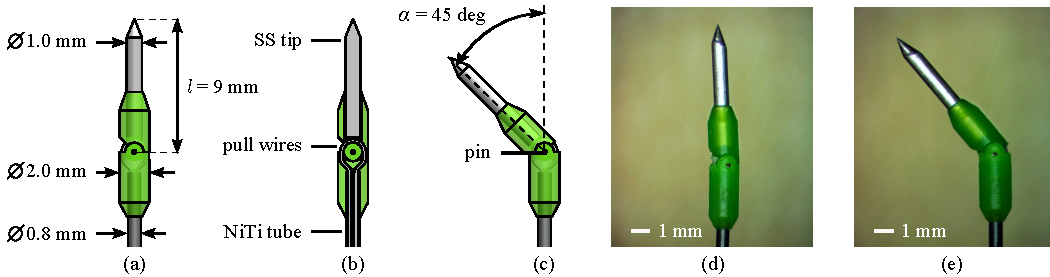
\includegraphics[width=\textwidth]{Images/Chapter3/ArticulatedTipDetail/ArticulatedTipDetail}
\caption[Articulated-tip needle mechanism]{The articulated-tip needle mechanism: (a) Schematic of the articulated tip in the straight configuration. The tip consists of a two-part 3D-printed hinge mechanism approximately 2.0 mm in diameter, secured to a 0.8-mm Nitinol tube, and a 1.0-mm ground stainless-steel tip. (b) Section view of the articulated tip in the straight configuration. A single continuous, pretensioned Nitinol pull wire is used to articulate the needle tip. The pull wire runs through the tubular Nitinol (NiTi) needle shaft, through channels in the proximal hinge section, and is secured to the distal hinge section with adhesive. A ground conical stainless-steel (SS) tip is secured to the distal hinge section with adhesive. (c) Schematic of the articulated-tip in the bent configuration. Nominal tip parameters of $l =$ 9~mm and $\alpha =$ 45~degrees were selected. (d) Micrograph of the assembled tip in the straight configuration. (e) Micrograph of the assembled tip in the bent configuration.}
\label{fig:ArticulatedTipDetail}
\end{figure*} 

A 0.13-mm Nitinol pull wire runs through the length of the needle shaft, through channels in the proximal hinge section, and is secured to the distal hinge section using epoxy adhesive. This pull wire is wound around a cable pulley in the needle hub, as described below, and allows actuation of the articulated tip. For reasons we describe in Section~\ref{sec:ArticDiscussion}, the articulated-tip needle is switched between fully straight and fully bent. Contact between the mating hinge components limits the range of motion in both directions. In the current design, tip length $l$ is 9~mm, while tip angle $\alpha$ is approximately 45 degrees. (Because of the manufacturing tolerances of the hinge components the actual maximum value of $\alpha$ was about 3 degrees less than the nominal value.) This tip geometry was selected based on the results of Section~\ref{sec:TipGeometryAnalysis}, and the strength limits of the plastic hinges. Although bent-tip needles with $l = 12$~mm had the smallest average radius of curvature in Section~\ref{sec:TipGeometryAnalysis}, the plastic hinge material was not able to support such long tips without occasionally failing.

\begin{figure*}[!h]
\centering
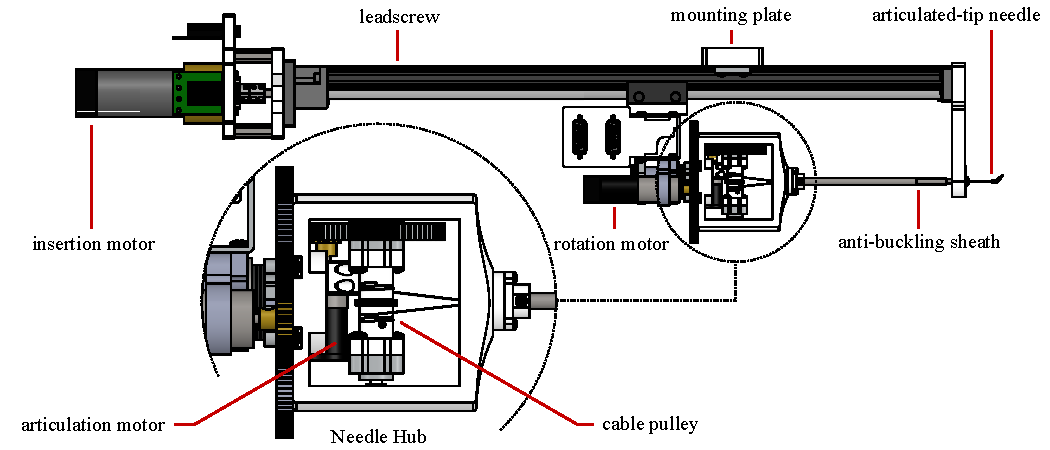
\includegraphics[width=0.6\textwidth]{Images/Chapter3/NS2Robot/NS2Robot}
\caption[Top view of the articulated-tip robot]{Schematic top view of the articulated-tip needle steering robot. DC motors drive a leadscrew for insertion of the needle, a rotary stage for rotation of the needle, and a cable pulley for articulation of the tip. A telescoping sheath prevents the flexible steerable needle from buckling outside of tissue. A detail view shows the removable needle hub attached to the rotatory stage. The needle steering robot is attached to a passive positioning arm using a mounting plate. A standard introducer sheath and connecting luer-lock fixture are omitted.}
\label{fig:NS2Robot}
\end{figure*}

\subsubsection{Needle Hub}
Fig.~\ref{fig:NS2Robot} includes a detail view of the articulated-tip steerable needle hub. The needle hub is a 3D-printed shell that mates to the rotary platform of the needle steering robot. Within the hub is a bearing-mounted cable pulley attached to a spur gear. The spur gear meshes with a pinion gear driven by a DC motor mounted on the rotary platform. The steerable needle shaft and anti-buckling sheath are also both affixed to the needle hub, and the entire needle/sheath assembly is removable from the needle steering robot.

\subsubsection{Needle Steering Robot}
Fig.~\ref{fig:NS2Robot} shows a schematic overview of the new robot designed to drive articulated-tip steerable needles. The robot is similar to the one described in~\cite{Majewicz2012}, but with an additional degree of freedom for the active articulation of the needle tip. The robot incorporates three DC motors: one drives a leadscrew for insertion of the needle, one drives a rotary platform that allows rotation of the needle hub, and one drives the cable pulley that allows articulation of the needle tip. A clamping plate allows the entire needle steering robot to be mounted on a passive positioning arm, which is attached to the standard rails on an operating room table. 

\subsection{Experimental Validation}

\subsubsection{Method}
\textit{Ex vivo} porcine liver tissue obtained fresh from a local butcher was used to simulate human liver tissue in all testing of the articulated-tip needle. Fig.~\ref{fig:ExperimentalSetupArticulatedTip} shows the experimental setup used in validation testing. We evaluated our articulated-tip steerable needle design in three ways. 

\begin{figure}[!t]
\centering
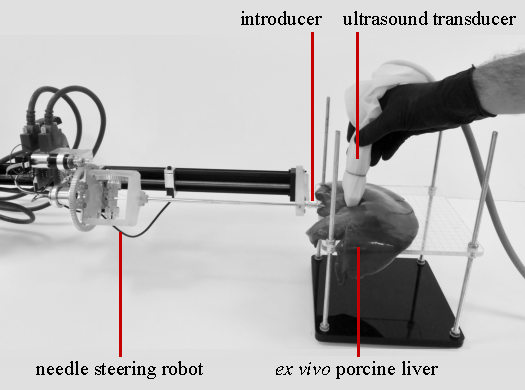
\includegraphics[width=0.6\columnwidth]{Images/Chapter3/ExperimentalSetup/ExperimentalSetup}
\caption[Setup for validation testing of the articulated-tip needle]{Experimental setup for validation testing of the articulated-tip steerable needle. The needle steering robot is mounted on a passive positioning arm. \textit{Ex vivo} porcine liver was used to simulate human liver tissue. The articulated-tip needle entered the liver tissue through a 13-gauge introducer sheath. A tracked 2D ultrasound transducer was used to image the needle for validation. }
\label{fig:ExperimentalSetupArticulatedTip}
\end{figure} 

First, to evaluate the articulation mechanism, the tip angle in the bent configuration was compared in free space and in liver tissue. To evaluate the tip angle in free space, the tip was imaged using a microscope with a digital camera attachment. The distal tip section and needle shaft were manually segmented from the micrograph, and the tip angle was measured. To evaluate the angle in tissue, the tip was articulated under 2D ultrasound imaging. The distal tip section and needle shaft were manually segmented from the ultrasound images, and the tip angle was measured.

Second, to evaluate the radius of curvature achieved by the articulated-tip needle, we performed a number of minimum-radius-of-curvature insertions (i.e., insertions with the tip kept in the bent configuration) in liver tissue. Each insertion was performed in a new section of liver to keep the needle from following an established track. After insertion stopped, the needles were scanned and segmented using the same method described in Section~\ref{sec:TipGeometryAnalysis} for the bent-tip needles.

Finally, we compared the articulated-tip needle design with bent-tip needles in a practical task, by performing a direction change maneuver with both needles. In this maneuver, the needle was inserted along a straight path for approximately 40~mm, before being steered with minimum radius of curvature in one direction for an additional 40~mm. The bent-tip needle was steered along the straight path using open-loop duty-cycle control, while the articulated-tip needle was inserted in the straight configuration. The needle was scanned and segmented after both the initial and final insertion steps, and the maximum deviation $\delta$ from the initial vector was measured. The bent-tip needle was the largest needle from Section~\ref{sec:TipGeometryAnalysis} that would fit through a 13-gauge introducer, with dimensions $l =$~4~mm and $\alpha =$~45~degrees (needle (a) in Fig.~\ref{fig:Bent-TipGeometry}).  

\begin{figure}[!t]
\centering
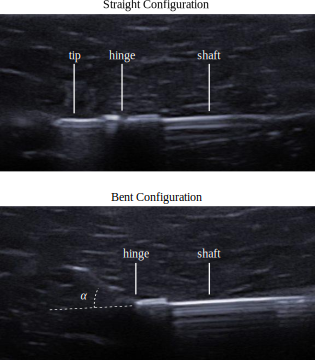
\includegraphics[width = 0.65\columnwidth]{Images/Chapter3/ArticulatedTipUS/ArticulatedTipUS}%
\caption[Ultrasound images of the articulated tip]{Ultrasound images of the articulated tip demonstrate the ability of the needle to achieve the straight (top) and bent (bottom) configurations in \textit{ex vivo} liver tissue. In the bent configuration, tip angle $\alpha$ was found to be 41.5 degrees using manual segmentation.}
\label{fig:ArticulatedTipUS}
\end{figure}

\begin{figure}[!t]
\centering
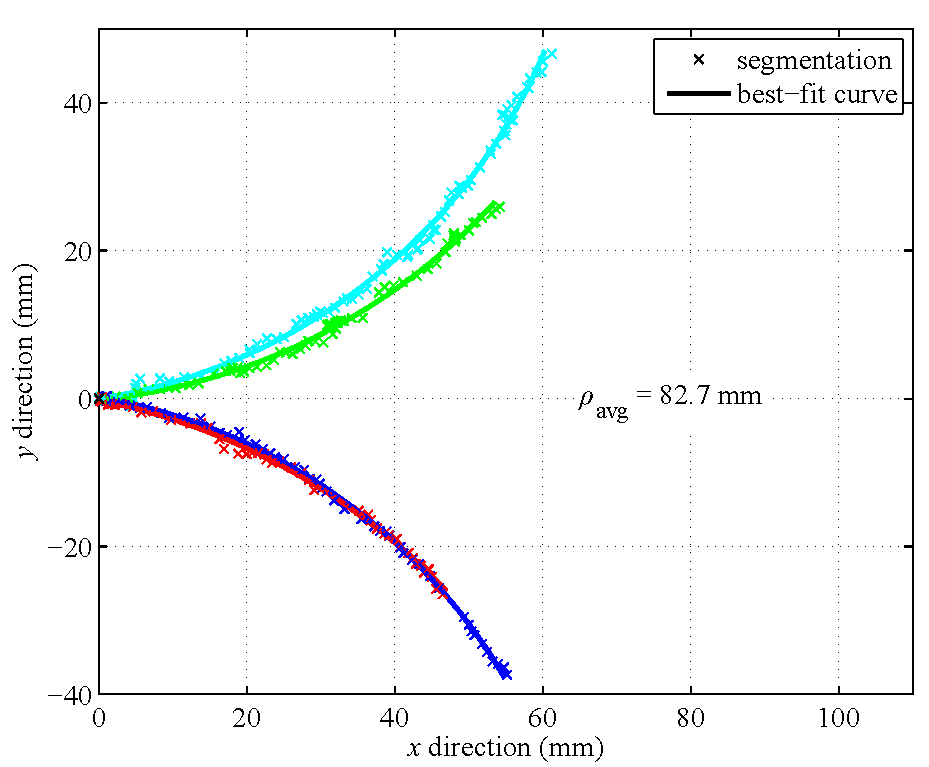
\includegraphics[width=0.75\columnwidth]{Images/Chapter3/ArticulatedTipMaxCurvature/ArticulatedTipMaxCurvature}
\caption[Minimum-$\rho$ results with the articulated-tip needle]{Minimum-radius-of-curvature results with the articulated-tip steerable needle. The needle was inserted with the articulated-tip in the bent configuration. Across four trials in fresh sections of \textit{ex vivo} liver tissue, the average radius of curvature $\rho_{\text{avg}}$ was 82.7~mm. The needle paths have been moved to a common origin for comparison.}
\label{fig:ArticulatedMaxCurvature}
\end{figure}  

\begin{figure*}[!ht]
\centering
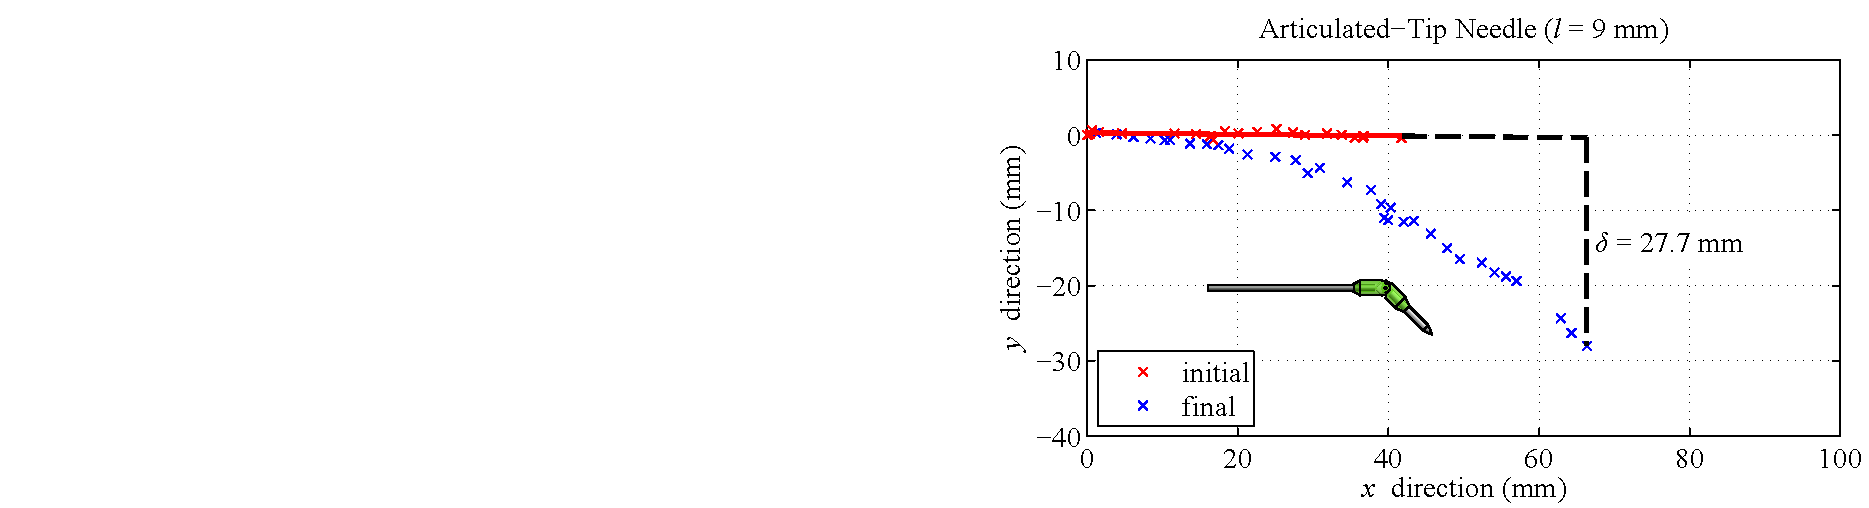
\includegraphics[width=0.75\textwidth]{Images/Chapter3/InsertAndTurn/InsertAndTurn1}
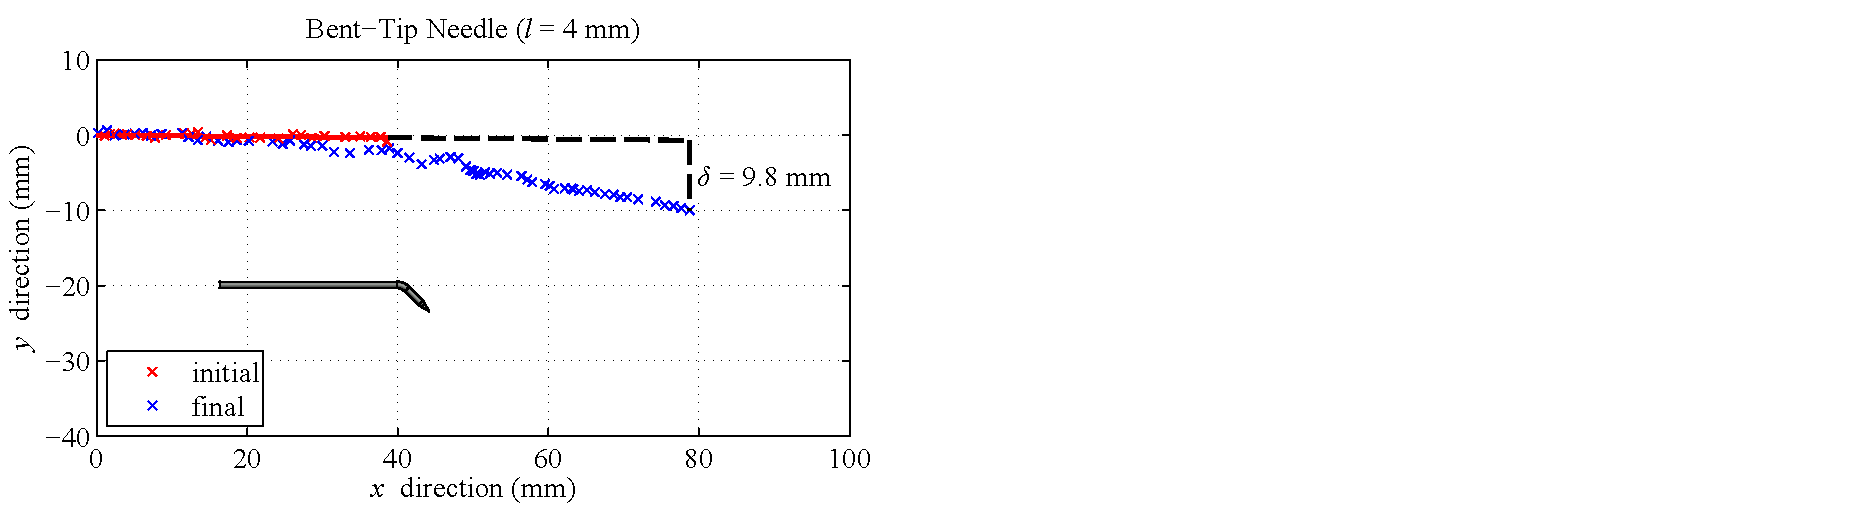
\includegraphics[width=0.75\textwidth]{Images/Chapter3/InsertAndTurn/InsertAndTurn2}
\caption[Maneuvers using bent-tip and articulated-tip needles]{Representative examples of direction change maneuver using a bent-tip needle with $l =$~4~mm and $\alpha =$~45~degrees, and an articulated-tip needle with $l =$~9~mm and $\alpha \approx$~45~degrees. Each needle was inserted along a straight path for approximately 40~mm, then was steered along the minimum-radius-of-curvature path for an additional 40~mm. In the maneuvers shown in the figure, deviation $\delta$ was 9.8~mm using the bent-tip needle, and 27.7~mm using the articulated-tip needle.}
\label{fig:InsertAndTurn}
\end{figure*}

\subsubsection{Results}
Fig.~\ref{fig:ArticulatedTipUS} shows ultrasound images of the articulated-tip needle in the straight and bent configurations. The needle steering robot was able to consistently articulate the needle tip to the same extent in tissue as in free space. In the micrographs shown in Fig.~\ref{fig:ArticulatedTipDetail}, the measured tip angle $\alpha$ was 41.1~degrees, while in the ultrasound images shown in Fig.~\ref{fig:ArticulatedTipUS}, the measured tip angle $\alpha$ was 41.5~degrees.

Fig.~\ref{fig:ArticulatedMaxCurvature} shows maximum curvature results for an articulated-tip needle with tip length $l =$~9~mm and tip angle $\alpha =$~45~degrees. Over the four tests shown in Fig.~\ref{fig:ArticulatedMaxCurvature}, the mean curvature was 82.7~mm with a standard deviation of 4.9~mm.       

Fig.~\ref{fig:InsertAndTurn} shows segmentation results from representative examples of the direction change maneuver. Using a bent-tip steerable needle, the maximum deviation $\delta$ from the initial vector was 9.8~mm for the test shown. Using the articulated-tip steerable needle, the maximum deviation $\delta$ was 27.7~mm for the test shown. It can be seen in Fig.~\ref{fig:InsertAndTurn} that the proximal 40~mm of each steerable needle shaft was displaced after the direction change maneuver. The Nitinol needle shafts, which were stiffer than the surrounding liver tissue, relaxed into single smooth circular curves rather than forming segmented straight-to-curved paths. The relaxation of the needle shaft was especially visible for the articulated-tip needle, which exhibited greater displacement $\delta$ from the initial vector.

\subsection{Discussion}
\label{sec:ArticDiscussion}
Overall, the validation results described above demonstrate that an articulated-tip needle is able to achieve better curvature in liver tissue than the largest practical bent-tip needle ($l \approx$~4~mm). However, there are several issues with the current design, mostly related to construction of the miniature hinges, which we plan to address before applying the design in a live-animal model. In the current design, the hinge elements are an ABS-like plastic. We are currently exploring machining methods that will allow us to create stainless-steel hinge elements, in order to improve performance, robustness and biocompatibility. Because of their plastic construction, the current hinges occasionally fail if tip lengths longer than about 9~mm are used. Based on the results of Section~\ref{sec:TipGeometryAnalysis}, increasing the tip length to approximately 12~mm should reduce radius of curvature to meet the 50-mm design requirement for our procedure. The current design is also sized to pass through a 13-gauge introducer sheath. The overall diameter will need to be slightly reduced to pass through a 15-gauge introducer sheath, which is the largest size that is clinically acceptable for percutaneous RFA of liver tumors.

Unlike in the design of van de Berg et al.~\cite{vandeBerg2015}, in our current design we elected to actuate the tip in a binary sense at the limits of the range of travel (i.e., the needle tip is either fully straight or fully bent). This simplifies the control of actuation, since we no longer need to compensate for the compliance of the pull wires. 

Based on observing the needle under ultrasound imaging during articulation, the moving tip easily displaces the liver tissue, making it unlikely that tissue damage is occurring due to tissue stress in the lateral direction. Confirming this would require a detailed histological analysis, which is beyond the scope of this paper. During closed-loop image-guided needle steering, the articulated-tip needle is only rotated in the straight configuration. When the needle is curving in one direction and the steering control software (not described in this paper) determines the needle should curve in a different direction, insertion stops, the needle is switched to the straight configuration, the needle is rotated to the new desired orientation, the needle is switched to the bent configuration, and insertion continues. A more detailed analysis of schemes for closed-loop image-guided control of the articulated-tip needle will be the subject of future work.

Both the flexure-tip design described by Swaney et al.~\cite{Swaney2013} and the ball-and-socket design described by van de Berg et al.~\cite{vandeBerg2015} could potentially be used with the exaggerated tip geometries we have described. It is unclear how well the passive flexure-tip needle, which relies on an asymmetric bevel to achieve articulation, would work for larger tip lengths and tip angles. The passive flexure also requires duty-cycle control to achieve straight paths, which introduces practical issues such as sensor windup and torsional needle deflection. Active articulated tips can also be used to introduce recognizable motion signatures into medical image data, as in~\cite{Adebar2014}, in order to reduce the complexity of image segmentation.


%!TEX root = PhD_Thesis.tex
\chapter[Recursive Estimation of Needle Pose]{Recursive Estimation of Needle Pose for Ultrasound-Guided Needle Steering}

\section{Introduction}
Although ultrasound has many advantages as an imaging modality, it produces noisy data compared to CT or MR imaging. This is especially true when using high-frequency vibration and Doppler ultrasound imaging to segment a curved needle, as described in Chapter 2. While we demonstrated that this approach can reveal the curved shape of the needle, the resulting measurement error is large relative to the desired precision of percutaneous ablation. (Clinicians using medical image guidance systems can manually position needle tips within approximately 2~mm of a target in similar interventions~\cite{Crocetti2008}.) Manual localization of a steerable needle in ultrasound data, which is described in this chapter, also involves large amounts of measurement noise. A further difficulty is that ultrasound imaging provides infrequent measurements, as the result of the low volumetric framerate of 3D imaging. 

In this chapter, to attain clinically relevant targeting precision using sparse, noisy measurements, we describe a model-based recursive estimation scheme known as an unscented Kalman filter (UKF). This filter relies on experimental quantification of process and measurement noise for ultrasound-guided needle steering in biological tissue, which was performed using an electromagnetic tracking system as a reference.
 
This chapter is divided into two main sections. Section~\ref{sec:UKF} describes our UKF estimation scheme. Section~\ref{sec:AutonomousControl} describes validation of the scheme through closed-loop steering experiments in simulation and bench-top tissue models. The work described in this chapter was published in the proceedings of the IEEE/RSJ International Conference on Intelligent Robotics and Systems~\cite{Adebar2014a}.

%======================================================================
\section{Estimation Scheme}
%======================================================================
\label{sec:UKF}
\subsection{Needle Steering Model}
Our kinematic model of needle steering is based on the unicycle model of steerable needle motion~\cite{Park2005,Webster2006}; we assume the needle travels along curved path sections that are tangent to each other. To begin, we define the needle tip frame. As shown in Fig.~\ref{fig:NeedleKinematics}, this frame is attached to the tip of the steerable needle, and oriented so that its \textit{z}-axis is tangent to the needle at the tip, and its \textit{y}-axis points towards the center of curvature. In this model, the state of the needle is described by the pose of the needle tip frame relative to a reference frame, in our case the 3D ultrasound frame or robot frame. 

\subsubsection{Needle State Representation}
Needle tip position is represented by a vector ${p} \in \mathbb{R}^3$. There are several possible representations of tip orientation, including quaternions, Euler angles, and axis-angle rotation vectors. We have elected to use a rotation matrix ${R} \in \textrm{SO(3)}$. This is a singularity-free representation. To describe differential rotations, we will also frequently use the axis-angle rotation vector representation $r \in \textrm{so(3)}$, which can be calculated directly from ${R}$. The state ${x}$ is thus defined as
\begin{align}
{x} = \{p \in \mathbb{R}^3, R \in \textrm{SO(3)}\}
\end{align}

\begin{figure*}[!t]
\centering
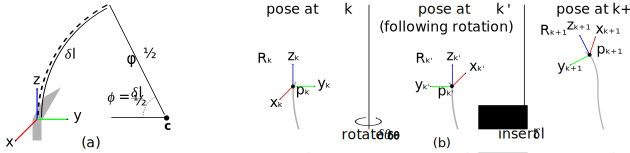
\includegraphics[width=\textwidth]{Images/Chapter4/NeedleKinematics/NeedleKinematics}%
\caption[Kinematic model of needle steering]{Kinematic model of needle steering~\cite{Webster2006} used in image-guided control: (a) Needle tip frame. The $z$-axis is tangent to the needle at the tip (ignoring the bevel or prebent section), the $y$-axis points towards the center of curvature. The needle path is an arc within the $y$-$z$ plane with radius $\rho$ and arc length $\delta l$. (b) Progression of the needle tip frame during steering. The steerable needle insertion is divided into increments, with incremental needle rotation angle ($\delta\theta$), incremental insertion distance ($\delta l$) and radius of curvature ($\rho$) updated as command inputs between increments. These command inputs define the transition of state vector ${x}$.}
\label{fig:NeedleKinematics}
\end{figure*}

\subsubsection{State Transition Model}
Based on the kinematic model of needle steering~\cite{Webster2006}, we define the transition of needle state to the next time interval, ${x_{k+1}}$, as a function of the current state, ${x_{k}}$, a vector of command inputs, ${u_{k}}$, and a vector of process noise, ${w}$:
\begin{align}
{x_{k+1}} = f({x_k}, {u_k}, {w}).
\end{align}
In our model, we divide needle steering into incremental insertions. Command inputs are applied between incremental insertions, and include change in needle base rotation $\delta\theta$, incremental insertion distance $\delta l$, and radius of incremental needle path $\rho$:
\begin{align}
{u} = \begin{bmatrix} \delta\theta & \delta l & \rho\end{bmatrix}^{\text{T}}.
\end{align}
The radius of the needle path can be experimentally measured as described in the previous chapters. The radius can also be adjusted using duty cycling~\cite{Minhas2007}, a control approach that uses short, variable periods of insertion with and without rotation to adjust needle curvature from maximum curvature to straight. System variability is modeled using nonadditive Gaussian noise in the state transition model. The noise ${w}$ can be separated into a position component, ${p_w} \in \mathbb{R}^3$, and an orientation component, ${R_w} \in SO(3)$. The index $k$ is omitted from the vector ${w}$ to signify the random nature of the vector.

The state transition function $f$ can be viewed as a transformation of the tip frame, as shown in Fig.~\ref{fig:NeedleKinematics}. The needle tip frame at time ${k}$ has pose defined by ${p_{k}}$ and ${R_{k}}$. The needle tip frame is first rotated about its $z$-axis by $\delta\theta$ to yield the rotated tip frame:
\begin{align}
{R_{k'}} = {R_{k}}{Rz}(\delta\theta).
\end{align}
The needle is then inserted a distance $\delta l$, with the tip following a circular path of radius $\rho$. From the definition of the tip frame shown in Fig.~\ref{fig:NeedleKinematics}, we know that the needle path will lie in the $y$-$z$ plane of the rotated frame defined by ${R_{k'}}$. The position of the needle tip after insertion relative to the rotated frame can be found directly from the geometry of the circular path:
\begin{align}
{^{k'}p_{k+1}} = \begin{bmatrix}0\\ \rho(1-\cos(\frac{\delta l}{\rho})) \\ \rho\sin(\frac{\delta l}{\rho})\end{bmatrix}.
\end{align}
Transforming this vector into the world frame, and including process noise yields an expression for $p_{k+1}$:
\begin{align}
{p_{k+1}} = {R_{k}}{Rz}(\delta\theta){^{k'}p_{k+1}}+{p_k} +{p_w}.
\end{align}
%\begin{align}
%\begin{array} {lcl} {p_{k+1}} & = & {R_{k}}{Rz}(\delta\theta){^{k'}p_{k+1}}+{p_k} +{p_w} \\ & = & {R_{k}}{Rz}(\delta\theta)\begin{bmatrix}0\\ \rho(1-\cos(\frac{l}{\rho})) \\ \rho\sin(\frac{l}{\rho})\end{bmatrix}+{p_k} +{p_w}.\end{array}
%\end{align}
The orientation of the tip frame after insertion can be defined using the same rotation matrices. Similar to other studies that have applied Kalman filters to orientation representations~\cite{Kraft2003}, we include orientation noise as an initial disturbance to the state vector, ${R_w}$.
The updated tip frame orientation is thus
\begin{align}
{R_{k+1}} = {R_{k}}{R_w}{Rz}(\delta\theta){Rx}\left(\begin{matrix}-\frac{\delta l}{\rho}\end{matrix}\right).
\end{align}
The vector ${r_{k+1}}$ is the rotation vector equivalent of ${R_{k+1}}$.

\subsubsection{Measurement Model}
Based on our 3D ultrasound needle segmentation method~\cite{Adebar2013}, we define the measurement model as full-state feedback with additive measurement noise vector ${v}$:
\begin{align}
{z_{k}} = {x_k} + {v}.
\end{align}
This model assumes that the automatic or manual segmentation method can measure the full 6DOF pose of the needle tip frame. Although rotation around the axis of a needle can not generally be resolved by 3D ultrasound, in the case of a curved steerable needle we can use the direction of needle curvature to estimate the $y$-axis of the needle frame.

\subsection{Unscented Kalman Filter}
The unscented Kalman Filter is an extension of the classical Kalman filter to nonlinear systems, and uses a set of sampled points around a mean value to represent distributions~\cite{Julier1997}. For brevity, we omit a detailed description of the typical UKF, and refer the reader to~\cite{Thrun2005} for a complete explanation. Our implementation of the UKF follows the original description of the algorithm~\cite{Julier1997}, with several modifications as described below. 

\subsubsection{Calculation of the Mean}
The first modification is our method for calculating the mean $\overline{x}$ of a set of states $x_0 \dots x_k$. In the UKF, this method is used to recover the mean and covariance of the state estimate from a set of transformed sigma points. Normally in a UKF, the state exists in a vector space, and can be represented by a vector $x \in R^n$. The mean of a set of vector states can be calculated as the sum of the states divided by the size of the set,
\begin{align}
\overline{x} = \frac{1}{k}\sum\limits_{i=1}^{k} x_i,
\end{align}
\noindent 
while the corresponding covariance can be calculated as:
\begin{align}
P = \frac{1}{k}\sum\limits_{i=1}^{k} (x_i-\overline{x})(x_i-\overline{x})^T.
\end{align}
\noindent
Our state includes the 3D position of the needle tip, represented by a vector ${p} \in \mathbb{R}^3$, and the 3D orientation of the needle tip, represented by a matrix ${R} \in \textrm{SO(3)}$. Because orientation is periodic, it is not possible to calculate the mean state or covariance using the above formulae. Instead, we use the iterative gradient descent approach proposed by Kraft~\cite{Kraft2003}. 

Given a set of state measurements $x_0 \dots x_k$, with each $x_i = \{p_i,R_i\}$, we calculate the mean position as:
\begin{align}
\overline{p} = \frac{1}{k}\sum\limits_{i=1}^{k} p_i.
\end{align}
We then calculate the set of equivalent axis-angle rotation vector representations $r_i \dots r_k$. To begin the gradient descent, we initialize the mean orientation estimate as $\overline{r} = r_0$. We define an orientation error in rotation matrix form as $E_i = R_i\overline{R}$, where $\overline{R}$ is again the equivalent rotation matrix representation of vector $\overline{r}$. Calculating this error for each of the $k$ orientations, we can form a measure of the difference between the current mean orientation estimate and the true mean orientation,
\begin{align}
\overline{e} = \frac{1}{k}\sum\limits_{i=1}^{k} e_i,
\end{align}
Since $\overline{e}$ is a rotation vector that points in the direction of the true mean orientation. The mean is then updated,
\begin{align}
\overline{R} = \overline{E} \overline{R}.
\end{align}
This correction is repeated until the norm of the adjustment vector $\overline{e}$ drops below an acceptable threshold ($1\times10^{-5}$ in our implementation).

\subsubsection{Calculation of the Covariance}
Calculating the covariance $P$ of a set of states $x_0 \dots x_k$ is straightforward after calculating the mean position and orientation as described. Comparing each state $x_i$ with the mean, we combine the position error with the calculated orientation error vector, to define a difference vector,
\begin{align}
d_i = \begin{bmatrix} p_i - \overline{p}\\ 
e_i
\end{bmatrix}.
\end{align}
The covariance $P$ can then be calculated directly as
\begin{align}
P = \frac{1}{k}\sum\limits_{i=1}^{k}dd^T.
\end{align}

\subsubsection{Injection of Process and Measurement Noise}
Since the effect of process noise on the state transition is nonadditive, we include the noise covariance matrices $Q$ and $R$ in the generation of the Sigma points. In other words, given a state estimate $\tilde{x} \sim N\left(\mu,P\right)$, we draw Sigma points from the distribution $\sim N\left(\mu,P+Q\right)$, and pass them through the state transition function.
 
%======================================================================
\section{Experimental Validation}
%======================================================================
\label{sec:AutonomousControl}
Application of the UKF requires an understanding of the relative amounts of uncertainty (\textit{i.e.}, noise) in the evolution of the state (process noise) and the measurement of the state (measurement noise). To quantify the process and measurement noise involved in 3D-ultrasound-guided needle steering, we first performed experimental measurements using samples of \textit{ex vivo} porcine liver tissue. We then validated our estimation scheme in simulated needle steering trials, and in bench-top needle steering experiments using the needle steering robot described in Chapter~2.

\subsection{Quantification of Process and Measurement Noise}
Process noise was quantified by using a magnetic tracking system to precisely measure the motion of a steerable needle tip during incremental insertion along constant curvature paths. A hollow steerable needle 0.80 mm in diameter was connected to the needle steering robot described in Chapter 2, and a 6DOF sensor attached to a magnetic tracking system (driveBAY; Ascension Technology Corp., Milton, VT) was inserted into the needle tip. The pose of the needle tip after each incremental step was compared with what was expected based on the previous pose and the process model. Denoting the state vector measured by the magnetic tracking system as $\hat{{x}}$, we determined an error vector ${w}$ at each step such that
\begin{align}
{\hat{x}_{k+1}} = f({\hat{x}_{k}}, {u_{\text{est}}}, {w}).
\end{align}
During these experiments, input vector ${u_{\text{est}}}$ was held constant at $[0, \text{3 mm}, \rho_{\text{est}}]^{T}$. The needle was inserted along four paths, with between fifteen and twenty measured positions per path. Initial tip frame orientation was measured by fitting a circular arc to the set of measured positions, and identifying the vectors tangent ($z$-axis) and normal ($x$-axis) to the arc at the initial tip position. Data analysis was performed offline using Matlab. 

The tip position measurements could be used directly, however the tip orientation measurements had to first be adjusted to conform to the definition of the needle tip frame given above. Specifically, the measured z-axis was aligned with the needle axis, but the measured x-axis and y-axis were not. To correct the orientation, a circular arc was fit to the measured tip points from each insertion, yielding an estimated radius of curvature $\rho_{est}$. The mean difference between the measured x-axes and the normal to the circular arc was used to correct the orientation measurements to be consistent with the needle tip frame.

Measurement noise was quantified by comparing automatic segmentation results from repeated 3D ultrasound scans of steerable needles in biological tissue. Between five and eleven repeated scans were performed for each of six needle tip poses. The needles were automatically segmented from each scan using the previously Doppler method described in Chapter 2. Data analysis was again performed offline in Matlab.

\subsection{Ultrasound-Guided Needle Steering Simulations}
We first evaluated our UKF algorithm in a series of simulated closed-loop needle steering trials. These simulations allowed us to compare our UKF results with the true needle tip state, which was not possible in the experiments described in the next section. In each trial, a target tip position and initial tip pose were identified in the 3D ultrasound coordinate system, and the needle tip was steered towards the target along a 3D path. Four initial scans were simulated to allow the UKF estimate to converge. Afterwards, the needle was steered in constant 3-mm incremental insertions using the UKF-filtered segmentation results to correct the needle rotation and path radius settings at each step. To provide a comparison baseline, each trial was also repeated using the unfiltered segmentation results as control feedback. 

The target point ${t}$ was varied according to a uniform distribution:
\begin{align}
{t} \sim U\left(
\begin{bmatrix} -20\\ 35\\ 30 \end{bmatrix},
\begin{bmatrix} 20\\ 65\\ 60 \end{bmatrix} \right).
\end{align}
Initial needle tip position was held constant: 
\begin{align*}
{p_{\text{init}}} = \begin{bmatrix} 0 & 50 & -40 \end{bmatrix}^{\text{T}}.
\end{align*}
Initial needle tip orientation was varied according to a normal distribution:
\begin{align}
{r_{\text{init}}} \sim N\left(
\begin{bmatrix} 0\\ 0\\ 0 \end{bmatrix},
\begin{bmatrix} 32.82 & 0 & 0\\ 0 & 32.82 & 0\\ 0 & 0 & 32.82 \end{bmatrix} \right).
\end{align}
Simulations were implemented in Matlab.

\subsection{Ultrasound-Guided Needle Steering Experiments}
In addition to simulation tests, we performed a series of closed-loop needle steering experiments. The robot steered a 0.58 mm needle with a bevel tip in \textit{ex vivo} porcine liver tissue under 3D ultrasound guidance. The UKF algorithm was implemented in C++ and combined with algorithms for Doppler image segmentation. A SonixMDP ultrasound console (Ultrasonix Medical Corp., Richmond, Canada) with a convex mechanical 3D transducer (4DC7-3/40) was used for imaging. Similar to the simulated trials, a target was defined in the 3D ultrasound coordinate system and the needle was steered in constant 5-mm incremental insertions using sensor feedback to correct the needle rotation and path radius settings at each step. For comparison, six steering tests each were performed with and without the UKF.

\section{Results}
\subsection{Quantification of Process and Measurement Noise}
Across 66 samples of process noise, the mean position error (in millimeters) and mean orientation error (in degrees) were \[{\overline{p}_{w}} = \begin{bmatrix} 0.38 &-0.09 &0.17 \end{bmatrix}^{\text{T}}, {\overline{r}_{w}} = \begin{bmatrix} 0.43 &0.02 &0.50 \end{bmatrix}^{\text{T}}.\] To find the best-fit zero-mean Gaussian distribution to the process noise, we reflected the measured noise vectors, resulting in a sample covariance of
\begin{align*}
{\hat{Q}} = \begin{bmatrix} 
\phantom{-}0.39 	& -0.06 	& \phantom{-}0.15 		& \phantom{-}0.24 		& -0.05 	& \phantom{-}0.08\\ 
-0.06 			& \phantom{-}0.21  	& -0.10   	& -0.17 	& \phantom{-}0.17 		& -0.05\\
\phantom{-}0.15 	& -0.10 	& \phantom{-}0.16    	& \phantom{-}0.09 		& -0.08 	& \phantom{-}0.23\\
\phantom{-}0.24 	& -0.17 	& \phantom{-}0.09  	& \phantom{-}0.65 		& -0.34 	& -0.09\\
-0.05 	& \phantom{-}0.17		& -0.08 	& -0.34 	& \phantom{-}1.22		& \phantom{-}0.00\\
\phantom{-}0.08 	& \phantom{-}0.05		& \phantom{-}0.23  	& -0.09 	& \phantom{-}0.00 	& \phantom{-}2.49\\
\end{bmatrix}.
\end{align*}

In the measurement noise experiment, we assumed the mean of repeated segmentations at each tip pose was the true needle pose. This was necessary because we did not have a reference segmentation method for comparison (thin steerable needles are not generally visible in B-mode ultrasound). Across 60 observations of measurement noise, the sample covariance was
\begin{align*}
{\hat{R}} = \begin{bmatrix} 
\phantom{-}0.81 & \phantom{-}0.09 & -0.27 & \phantom{-}3.41 & \phantom{-}37.1 & \phantom{-}18.2\\ 
\phantom{-}0.09 & \phantom{-}1.10 & \phantom{-}0.51 & -17.7 & \phantom{-}20.2 & \phantom{-}4.97\\
-0.27 & \phantom{-}0.51 & \phantom{-}0.90 & -13.5 & \phantom{-}1.54 & -3.68\\
\phantom{-}3.41 & -17.7 & -13.5 & \phantom{-}3930 & -1720 & -375\\ 
\phantom{-}37.1 & \phantom{-}20.2 & \phantom{-}1.54 & -1720 & \phantom{-}7520 & \phantom{-}2740\\ 
\phantom{-}18.2 & \phantom{-}4.97 & -3.68 & -375 & \phantom{-}2740 & \phantom{-}1240\\
\end{bmatrix}.
\end{align*}
These experimental results give an indication of the relative levels of process and measurement noise, which is valuable for a Kalman filter formulation; however, only a relatively small number of measurements were practical for both experiments, and as a result it is difficult to infer characteristics of the underlying distributions. On the other hand, the process noise measurements, which were correlated and had non-zero mean, suggest that the kinematic model of needle steering we applied may not completely capture needle behavior in \textit{ex vivo} liver. While a more sophisticated bicycle model of needle kinematics exists~\cite{Webster2006}, it is identical to the unicycle model except when rotating the needle, which we did not do in our process noise experiments. With a more accurate kinematic model, we would expect the process noise to approximately follow a normal distribution with zero mean. This process noise would describe small deflections of the needle tip off the expected trajectory that would result from steering in an inhomogeneous biological material. The difference in the experimental measurements suggests further investigation is warranted.  

\begin{figure}[!t]
\centering
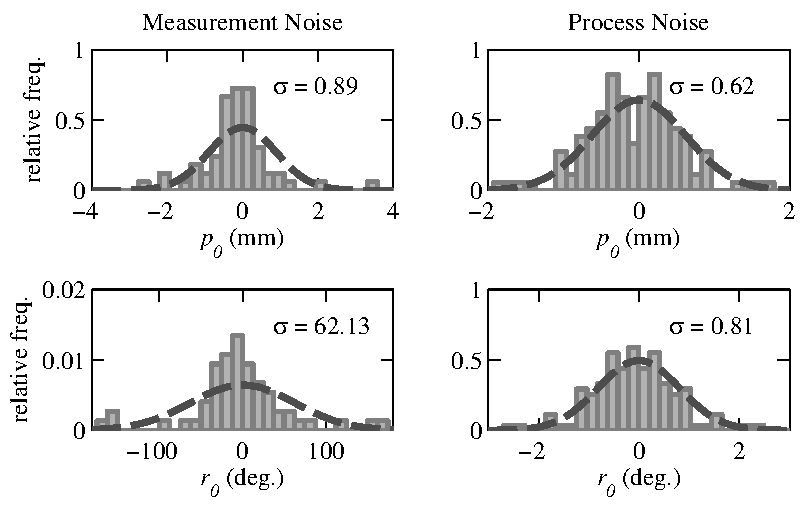
\includegraphics[width=0.75\columnwidth]{Images/Chapter4/Noise/Noise}%
\caption[Distributions of process and measurement noise]{Distributions of process and measurement noise for $p_0$ and $r_0$ components of position and orientation. Histograms of experimentally measured error vectors (gray bars) are compared with the normal distributions used in needle steering simulations.}
\label{fig:Noise}
\end{figure}

To make our simulations realistic, we chose to formulate the Kalman gains in the UKF without exact knowledge of the process or measurement noise distributions. Specifically, the UKF assumed both process and observation noise were uncorrelated and normally distributed with zero mean and variances of 
\begin{align*}
{Q} = \text{diag}(\begin{bmatrix} 0.2 & 0.2 & 0.2 & 3.28 & 3.28 & 3.28 \end{bmatrix}^{\text{T}}),
\end{align*}
\begin{align*}
{R} = \text{diag}(\begin{bmatrix} 1 & 1 & 1 & 3282 & 3282 & 3282 \end{bmatrix}^{\text{T}}).
\end{align*}

\subsection{3D-Ultrasound-Guided Needle Steering Simulations}
Over 10,000 simulation trials, the average error (mean~$\pm$~standard deviation) in final tip placement was 2.26~$\pm$~1.30~mm using the UKF-filtered segmentation results for feedback, and 11.85~$\pm$~7.36~mm using the unfiltered segmentation results. Based on a bootstrapped statistical test, the UKF resulted in a statistically significant increase in placement accuracy ($p~<~0.01$).

\begin{figure}[!h]
\centering
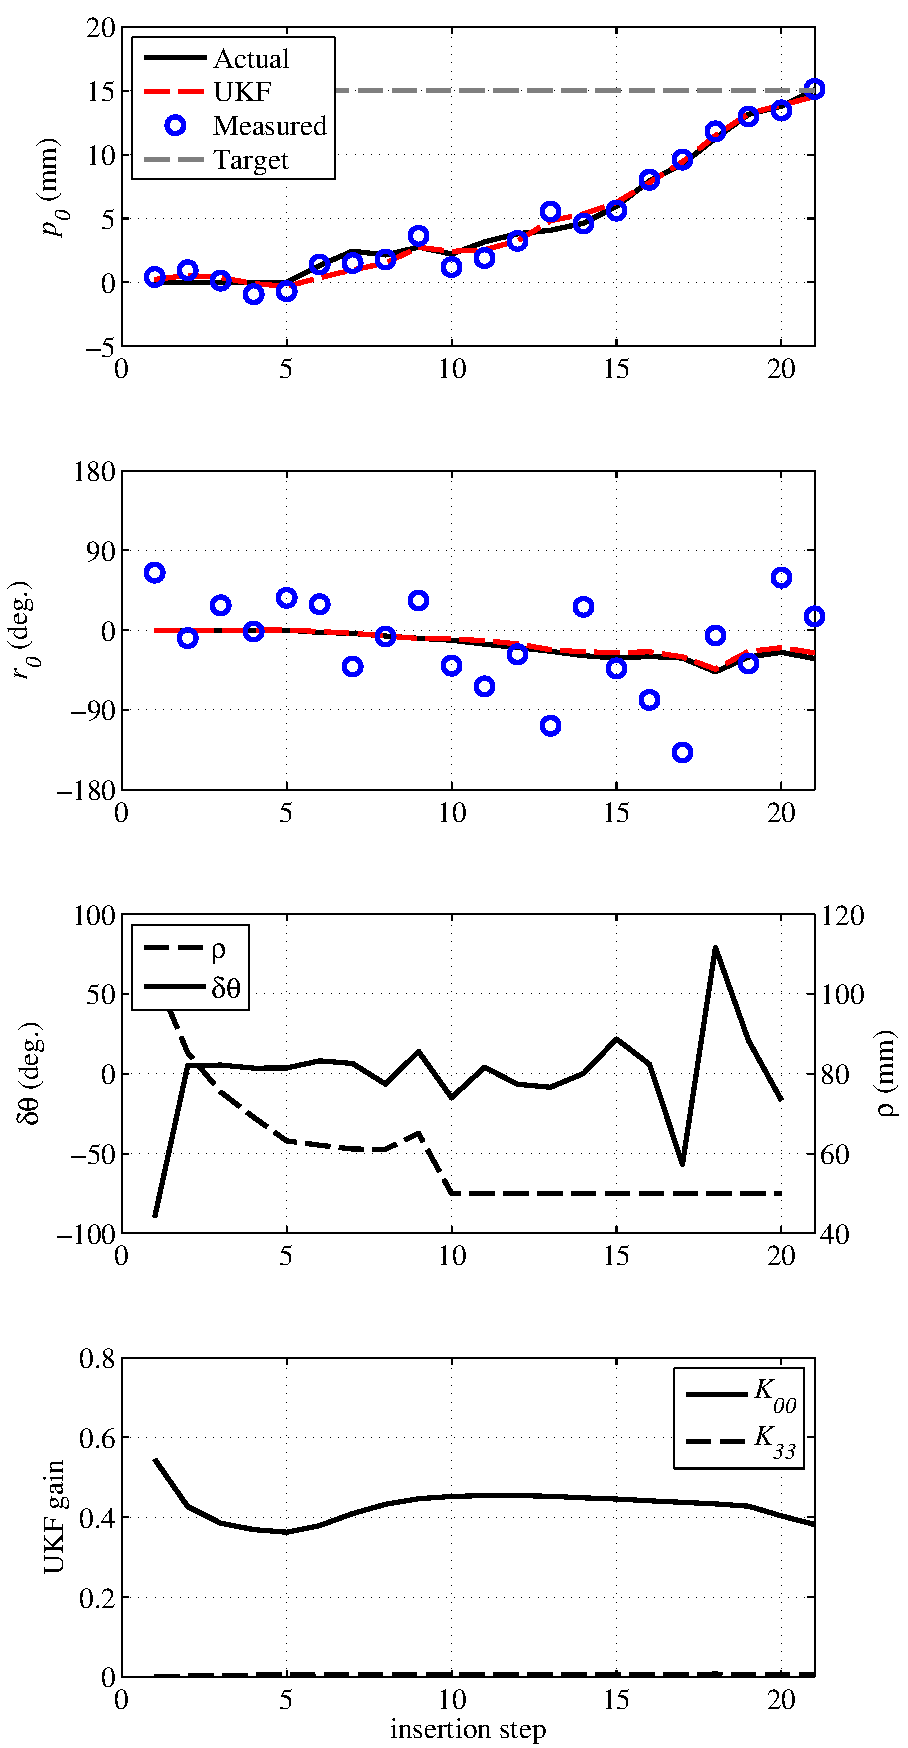
\includegraphics[width=0.5\columnwidth]{Images/Chapter4/SimulationResults/SimulationResults}%
\caption[Closed-loop needle steering results]{Closed-loop needle steering results. Actual, measured and UKF-estimated state vector elements $p_0$ and $r_0$ are shown for steering towards a target located at $p_0 = 15$. The resulting values of control variables $\delta\theta$ and $\rho$ are also plotted, and represent the control effort needed to overcome process variability inherent to steering in biological tissue. UKF gain values $K_{00}$ and $K_{33}$ show significant reliance on measured needle position, but relatively little reliance on measured needle orientation when forming the UKF estimate. }
\label{fig:SimulationResults}
\end{figure}   

Fig.~\ref{fig:Noise} shows experimental histograms of process and measurement noise for the first components of position and orientation (\textit{i.e.}, $p_0$ and $r_0$) compared to normal distributions with the same variance. In our needle steering simulations, we modeled the process and measurement noise as normally distributed, with zero mean and covariance equal to ${\hat{Q}}$ and ${\hat{R}}$ as defined above.

\begin{figure}[!t]
\centering
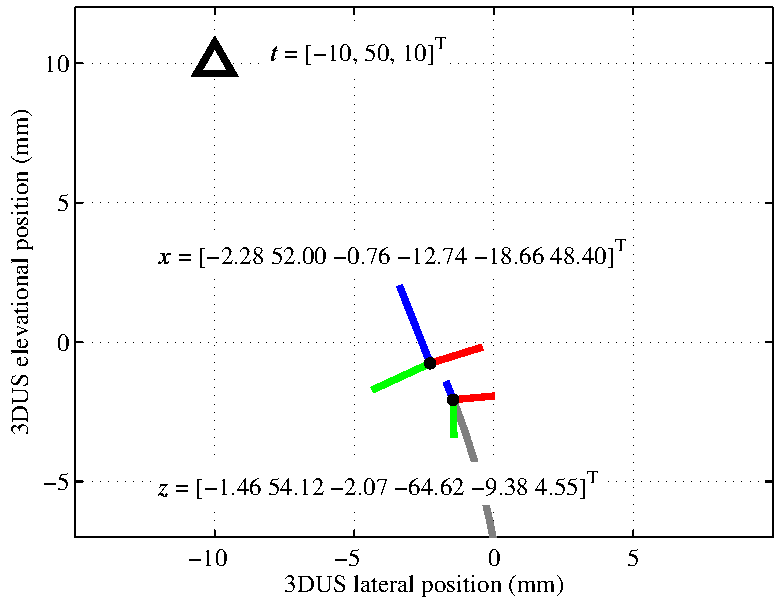
\includegraphics[width=0.7\columnwidth]{Images/Chapter4/ExperimentalResults/ExperimentalResults}%
\caption[Results using UKF in autonomous control]{Experimental results for closed-loop needle steering in \textit{ex vivo} porcine liver tissue. After seven iterations, the UKF estimate of needle pose ${x}$ (large axes) has less error in orientation than the measured needle pose ${z}$ (small axes), which is based entirely on the segmented needle curve (solid line). The robot continued steering towards the target point ${t}$, and achieved final placement error of 2.67 mm.}
\label{fig:ExperimentalResults}
\end{figure}

Fig.~\ref{fig:SimulationResults} shows simulation results from using the UKF-filtered segmentation data in closed-loop steering towards a target. The figure shows actual, measured and estimated values for two state elements (again $p_0$ and $r_0$), along with resulting control inputs ($\delta\theta$ and $\rho$) and UKF gains. In this simulation, the needle tip was steered from a point with $p_0 = 0$ towards a point at $p_0 = 15$. As seen in the figure, the UKF approach accurately estimated the true position and orientation despite large amounts of measurement noise, particularly in orientation. As mentioned above, the segmentation method we apply is based on measuring the centroid of irregular Doppler patches around the needle, and gives a relatively poor indication of needle tip orientation. The UKF estimate of tip orientation was thus based almost entirely on our kinematic model of needle steering, whereas the UKF estimate of tip position was based on both the kinematic model and the segmentation results. This is shown by the UKF gains $K_{00}$ and $K_{33}$, which represent how heavily measurements $z_0$ and $z_3$ are weighted versus the corresponding process model outputs at each iteration. As shown by the control inputs, the robot made a large initial rotation to steer the needle towards the target, then made small corrections as a result of the steering variability (process noise). Once the needle approached the target, larger rotations and tighter path radii were necessary to correct for variations. At the end of the trial the needle tip was 0.83 mm from the target.    

\subsection{3D-Ultrasound-Guided Needle Steering Experiments}
Table~\ref{table:Targeting Results} lists final tip placement error for each closed-loop steering test. Over six tests using the UKF, the average error was 2.69 mm. This is within one standard deviation of the mean simulation result, and approaches an acceptable error for clinical applications. Over six tests without the UKF, the average error was 11.39 mm, which is also within one standard deviation of the mean simulation result. The robot executed between nine and twelve incremental insertions in each test. 

\begin{table}[!h]
% increase table row spacing, adjust to taste
\renewcommand{\arraystretch}{1.3}
\centering
\caption{Tip placement errors in needle steering experiments}
\label{table:Targeting Results}
% Some packages, such as MDW tools, offer better commands for making tables
% than the plain LaTeX2e tabular which is used here.
\begin{tabulary}{\columnwidth}{| l | C | C | C | C | C | C | C |}
\hline
Test & 1 & 2 & 3 & 4 & 5 & 6 & avg. \\
\hline
UKF (mm) & 2.67 & 2.34 & 3.83 & 3.44 & 2.90 & 0.98 & 2.69 \\
\hline
No UKF (mm) & 9.89 & 13.41 & 9.03 & 11.12 & 10.14 & 14.74 & 11.39 \\
\hline
\end{tabulary}
\end{table}

Fig.~\ref{fig:ExperimentalResults} shows results from Test 1 with the UKF. In this test, the needle tip was intially located at ${p}~=~\begin{bmatrix} -0.80 & 53.26 & -14.04 \end{bmatrix}^{\text{T}}$ mm, and was steered towards the target at ${t} = \begin{bmatrix} -10 & 50 & 10 \end{bmatrix}^{\text{T}}$ mm. The figure shows the segmented needle curve, measured tip frame, and UKF-estimated tip frame after seven UKF iterations (four initial scans and three incremental insertions). At this point the UKF-estimated tip position was close to the measured tip position; however, the UKF-estimated tip orientation was significantly different from the measured tip orientation. This example illustrates the importance of the UKF in closed-loop robot control, since using the segmentation results directly would have caused the robot to falsely correct the needle orientation with a large rotation.     



%!TEX root = PhD_Thesis.tex
\chapter[Human-in-the-Loop Control]{Human-in-the-Loop Control of Ultrasound-Guided Needle Steering}

\section{Introduction}
The experimental results presented in Chapter 4 showed promising accuracy in autonomous targeting of the needle tip. While these tests were performed in biological tissues, they were completed in a bench-top setting, over a relatively small needle steering workspace. Early tests in a more realistic clinical environment---using a porcine cadaver in a simulated interventional radiology suite---revealed several problems preventing the direct application of our bench-top techniques. The mechanical 3D ultrasound transducer used in the previous section has limited field of view relative to the size of the liver, and any motion of the transducer invalidates all existing data. (In Section~\ref{sec:AutonomousControl} the transducer was clamped relative to the tissue sample.) External tracking systems can be used to increase the ultrasound's field of view by creating panoramic data, but this necessitates additional infrastructure. The appearance of the vibrating needle in Doppler ultrasound can be highly irregular in more realistic imaging arrangements. The Doppler approach still provides an indication of needle pose, but more sophisticated segmentation algorithms would be needed for autonomous control as in Section~\ref{sec:AutonomousControl}. Finally, visualization of 3D ultrasound data, needle pose, target location, etc. requires specialized software.

To allow closed-loop ultrasound-guided needle steering in a realistic clinical situation, we implemented our UKF estimation scheme using a different imaging approach. Specifically, we used freehand-3D ultrasound imaging, and manual localization of the steerable needle tip. 

This chapter is divided into three sections. Section~\ref{sec:HumanInTheLoopImplementation} describes the algorithmic, hardware, and software implementation of our clinical human-in-the-loop approach. Section~\ref{sec:HumanInTheLoopValidation} describes experimental validation of our human-in-the-loop control approach, in bench-top and simulated clinical testing. Section~\ref{sec:HumanInTheLoopResults} presents the results.

\section{Implementation}
\label{sec:HumanInTheLoopImplementation}

\subsection{Robot and Steerable Needles}
\label{sec:NS2RobotAndNeedle}
Chapter 3 presented a new articulated-tip steerable needle that showed promising curvature results in biological tissue. Unfortunately, as discussed in that chapter, the plastic construction of the miniature hinges failed too frequently to be used in a clinical setting. Chapter 6 discusses possible future improvements to the hinge design. In this chapter, we applied the exaggerated tip geometry suggested by the results of Chapter 3, but used a flexure tip, consisting of a rectangular Nitinol wire plastically deformed to the desired tip angle. This tip is able to pass through an introducer sheath, because of the large elastic range of Nitinol, and while returning to its bent shape inside tissue. This design does require duty cycle control to follow straight paths, and may increase tissue damage, unlike the articulated-tip needle. A similar flexure tip was previously proposed by Swaney et al.~\cite{Swaney2013}. Fig.~\ref{fig:NS2AndNeedle} shows the flexure tip steerable needle and the robot used to drive it in this chapter.

\begin{figure}[!ht]
\centering
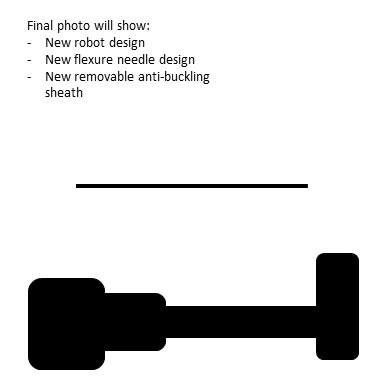
\includegraphics[width = 0.4\columnwidth]{./Images/Chapter5/NS2RobotAndNeedle/DRAFTNS2RobotAndNeedle.jpg}%
\caption[Robot and flexure-tip steerable needles]{Portable needle steering robot with positioning arm and handle, flexure-tip steerable with integrated anti-buckling sheath and connector fitting for introducer sheath.}
\label{fig:NS2AndNeedle}
\end{figure}  

\subsection{Control Modes}
Our implementation of human-in-the-loop control allows the user to select between joint-space control of the needle steering robot and task-space control of the needle tip position. In joint-space control, the user uses a 3D mouse (SpaceNavigator; 3Dconnexion, Boston, MA) to directly control the insertion and rotation of the needle steering robot's two DOF. Using a rate-control scheme, uniaxial displacement of the 3D mouse is mapped to insertion velocity, while uniaxial rotation of the 3D mouse is mapped to rotation speed. The remaining inputs of the 3D mouse are not used. Fig.~\ref{fig:InputDevices}

\begin{figure}[!t]
\centering
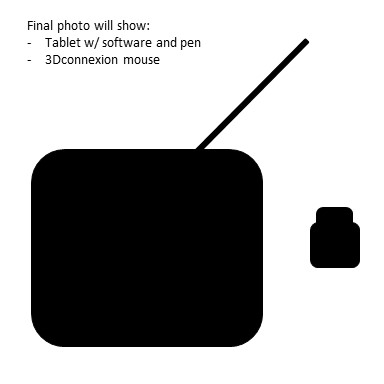
\includegraphics[width = 0.4\columnwidth]{./Images/Chapter5/InputDevices/DRAFTInputDevices.jpg}%
\caption[Input devices for robot control]{Input devices for human-in-the-loop control of robotic needle steer: (a) A 3D mouse is used for rate control of the steerable needle insertion and rotation. (b) A tablet is used to select targets and measure the needle tip position in the stream of 2D ultrasound images.}
\label{fig:InputDevices}
\end{figure}  

In task-space control, the user selects target positions directly in the live 2D ultrasound image using a tablet interface (Cintiq 13; Wacom Co., Vancouver, WA. The robot then steers the needle towards the target semi-autonomously, with feedback based on the output from the UKF estimation scheme described in Chapter 4. The estimator is updated without measurement feedback (i.e., based on the process model) at the ultrasound machine's native framerate. After every 10~mm of insertion, the system requires a tip position measurement, which the user provides by scanning over the needle tip and localizing it using the tablet interface. The estimation scheme is implemented exactly as described in Chapter 4 with two exceptions. First, the process and measurement noise levels were again experimentally characterized for the flexure needle and manual measurements, and the filter gains were adjusted accordingly. Second, the manual measurements only provided feedback on tip position, so tip orientation feedback was taken directly from the output of the estimator, with extremely low gain (high variance). This approach avoided practical computational issues related to matrix inversion and manipulation.

\begin{figure}[!t]
\centering
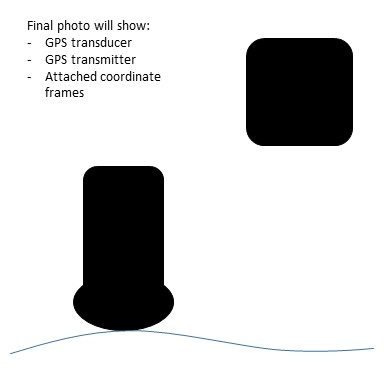
\includegraphics[width = 0.4\columnwidth]{./Images/Chapter5/Freehand3DUS/DRAFTFreehand3DUS.jpg}%
\caption[Freehand 3D ultrasound imaging arrangement]{Freehand 3D ultrasound imaging arrangement. The ultrasound transducer with integrated tracking element and electromagnetic tracking base station are depicted, along with the corresponding coordinate frames used to reconstruct the 3D pose of the 2D ultrasound image data.}
\label{fig:freehand3DUS}
\end{figure}  

\subsection{Freehand 3D Doppler Ultrasound Imaging}
As in the previous chapters, a SonixMDP ultrasound console (Ultrasonix Medical Corp., Richmond, Canada) was used for imaging. Unlike in the previous chapters, a 2D curvilinear transducer (C5-2/60) with an integrated electromagnetic tracking element was used. Fig.~\ref{fig:freehand3DUS} depicts this arrangement. The calibrated electromagnetic tracking system, branded as SonixGPS by Ultrasonix, allows the 3D context of the 2D ultrasound image data to be resolved in real time. 

As in Chapter 2, external vibrations were applied to the proximal end of the steerable needle shaft. However, in this chapter, a spring-loaded clip was used to attach a vibration motor (a miniature DC motor spinning a small eccentric mass) to the steerable needle shaft. Fig.~\ref{fig:Buzzer} shows the new vibration device. Compared to the integrated piezoelectric buzzer described in Chapter 2, this system has the advantages that is completely disposable if contaminated with bodily fluids, and it can be visually monitored during insertion and retraction to ensure good coupling. These characteristics were identified as necessary after early cadaver testing.

\begin{figure}[!t]
\centering
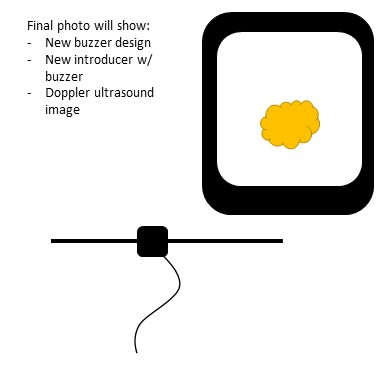
\includegraphics[width = 0.4\columnwidth]{./Images/Chapter5/Buzzer/DRAFTBuzzer.jpg}%
\caption[Disposable buzzer]{Disposable buzzer for ultrasound Doppler imaging. A 3D-printed spring-loaded clip attaches a vibration motor to the steerable needle shaft. The unit is battery powered and entirely disposable.}
\label{fig:Buzzer}
\end{figure}  

\subsection{Visualization and Control Software}
A custom graphical user interface (GUI) was developed using Qt for human-in-the-loop control. The GUI is shown in Fig.~\ref{fig:GUI}. The clinician user views both a live 2D ultrasound image streamed from the SonixMDP console, as well as a live 3D visualization of the robot pose, transducer pose, estimate, and target, as defined using the SonixGPS tracker. The GUI is optimized for a tablet interface. Controls allow the user to select between the two control modes (joint-space control and task-space control). The user can also use the tablet interface to set a the target point by clicking in the live 2D ultrasound image. Measurements of the steerable needle tip's position are similarly performed by clicking in the live 2D ultrasound image. 

\begin{figure}[!t]
\centering
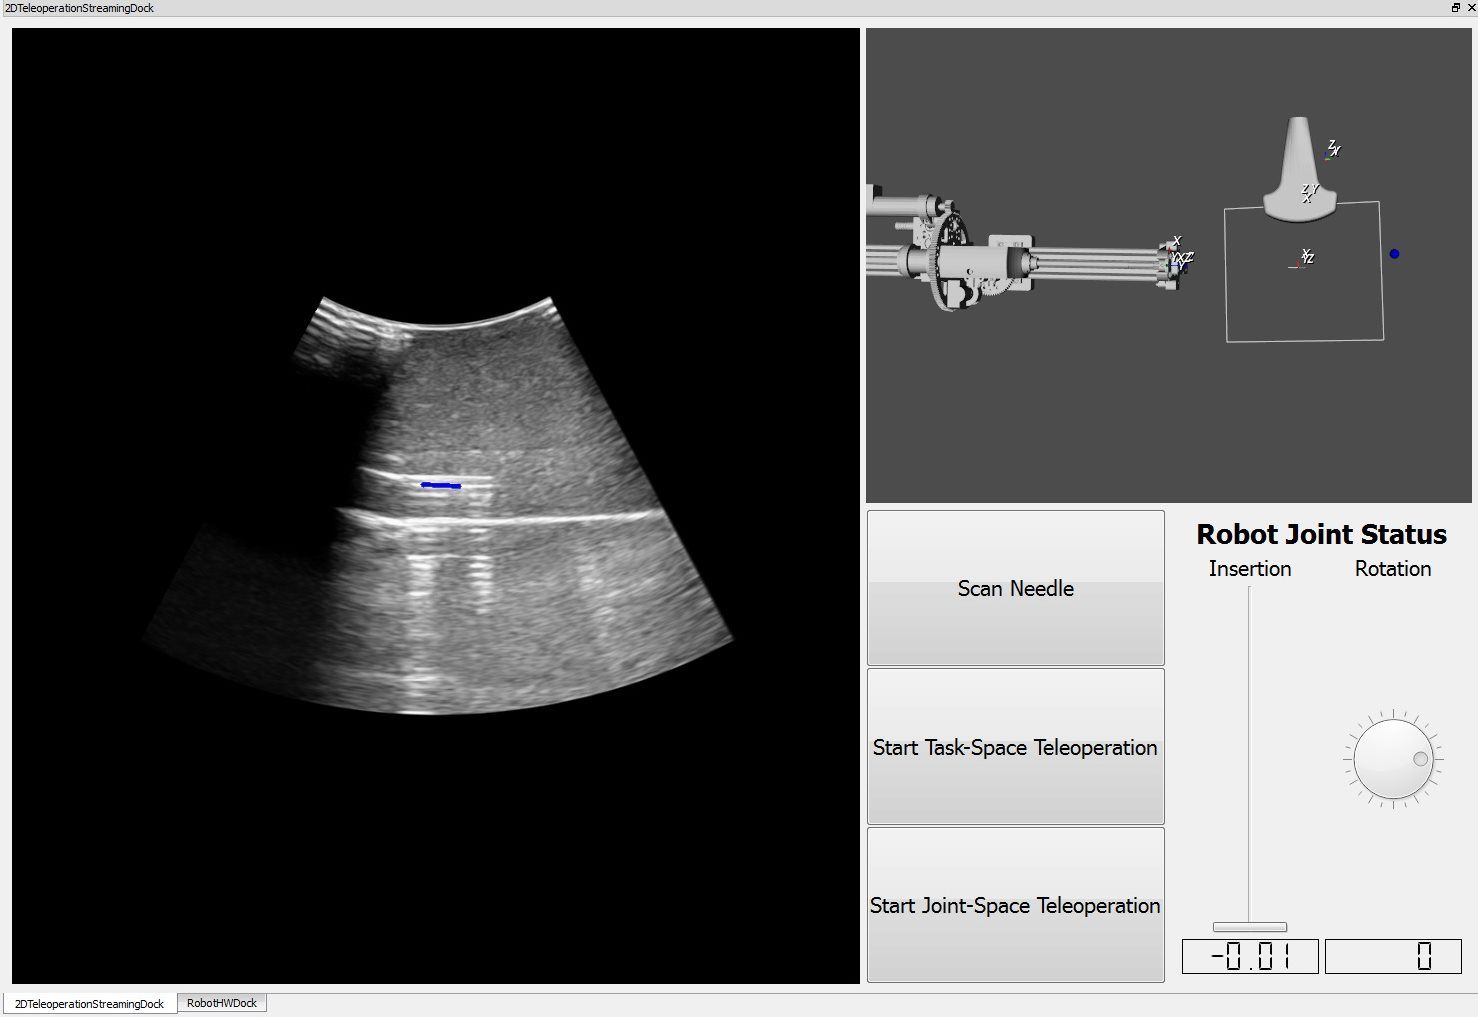
\includegraphics[width = 0.9\columnwidth]{./Images/Chapter5/GUI/GUI.jpg}%
\caption[Software interface]{Software interface for human-in-the-loop control. A screenshot shows the software during initial insertion of the robot, while the steerable needle tip is still within the introducer needle. Three panels are shown: (left) the live 2D ultrasound image with the current tip frame estimate over the hyperechoic needle shaft, (top right) the 3D visualization showing the ultrasound transducer pose, robot pose, tip frame estimate, and target (blue sphere), (bottom right) software control buttons and robot status readout.}
\label{fig:GUI}
\end{figure}  






\section{Experimental Validation}
\label{sec:HumanInTheLoopValidation}

\subsection{Quantification of Process and Measurement Noise}
As in Chapter 4, we first quantified process noise and measurement noise using our new robot and imaging arrangement. Process noise was again quantified by using a magnetic tracking system to precisely measure the motion of a steerable needle tip during incremental insertion along constant curvature paths. In this testing, a flexure-tip steerable needle with $l = 10$~mm and $\alpha = 45$~degrees was used. The needle was inserted along a minimum-radius-of-curvature path at a constant insertion velocity of XX mm/s, and no rotation. The pose of the needle tip after each incremental step was compared with what was expected based on the previous pose and the process model. Although the insertion increment varied slightly due to software timing, it was generally about 0.2~mm. The needle was inserted along six paths, with 617 total measurements captured. The initial tip frame orientation was defined in the robot frame based on fixture geometry and the initial joint values $\theta$ and $\l$. Radius of curvature $\rho$ for the needle was also measured using the magnetic tracking data and the least-squares fitting approach described in Chapter~3. Data analysis was performed offline using Matlab. 

Measurement noise was quantified by comparing manual tip localization results from repeated freehand-3D ultrasound scans of steerable needles in porcine liver tissue. Five repeated measurements were performed at each tip position, with 200 total measurements over five needle insertions. For each measurement, the user scanned over the needle with the ultrasound transducer, and manually selected the location of the steerable needle tip using the tablet and stylus. Data analysis was again performed offline in Matlab.

\subsection{Accuracy of Estimation Scheme}
We attempted to quantify the accuracy of our UKF estimation scheme in this application by comparison with a gold-standard measurement. This is difficult because there is no true gold-standard measurement of steerable needle tip pose (if there was, we would likely attempt to use it for closed-loop control in place of ultrasound imaging). Although an electromagnetic tracker inside the needle tip was used for quantifying process noise, there are several practical issues that limit its use as a gold-standard. First, the tracker is sensitive to electromagnetic noise from the vibration motor during actual steering. Second, the vendor-supplied calibration of the tracked ultrasound transducer is not perfectly accurate. Finally, it is impossible to place the electromagnetic transducer right at the needle tip (because of the rigid bent-tip section), so a tip calibration must be applied to the raw tracking data. This tip calibration can become inaccurate as the needle bends, and makes the measurement very sensitive to orientation noise. 

In any case, since the electromagnetic tracking system provides the best reference data, we compared our estimator with it over a series of steering trials. Over four insertions in \textit{ex vivo} porcine liver, the needle was steered while alternating between joint-space and task-space control. On each control update (synchronized to the ultrasound framerate), the calibrated electromagnetic tracker reading and UKF estimate was saved, and comparison was performed offline in Matlab.

\subsection{Clinical Needle Steering Experiments}
Fig.~\ref{fig:CadaverSetup} shows the experimental setup for the clinical needle steering experiments. A fresh pig carcass with an undisturbed liver was obtained for testing. To prevent coagulation and preserve the mechanical properties of the liver as much as possible, heparin was administered at a dosage of 300 IU/kg prior to euthanasia. The carcass was placed in supine position on a standard interventional radiology suite table, and was restrained to prevent tissue motion. 

\begin{figure}[!t]
\centering
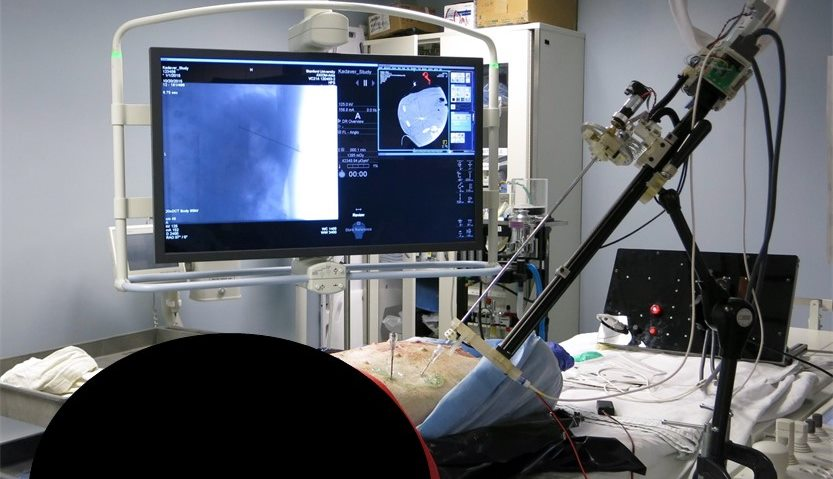
\includegraphics[width = \columnwidth]{./Images/Chapter5/CadaverSetup/CadaverSetup.jpg}%
\caption[Clinical Needle Steering Experimental Setup]{Clinical Steering Experimental Setup. The pig carcass is mounted in supine position on the table. The needle steering robot is secured to the table rails, and connected to an introducer sheath to allow access to the liver through skin and subcutaneous fat. A second introducer sheath allows placement of target coils.}
\label{fig:CadaverSetup}
\end{figure}  

After exploratory ultrasound imaging, multi-loop-coil fiducials were implanted in the liver to serve as targets. These fiducials are designed to be visible in CT imaging, but are also visible in ultrasound because of the gas trapped in the coils.  

A second 15-gauge introducer needle was used to place each fiducial. 

The needle was left in place during steering to aid in target identification.

After implanting each target, the needle steering robot was used to place the tip of the steerable needle at the target fiducial using human-in-the-loop control. 

The steerable needle accessed the liver in an anterior subcostal approach, through a 15-gauge, XX-cm introducer needle. 

\begin{figure}[!t]
\centering
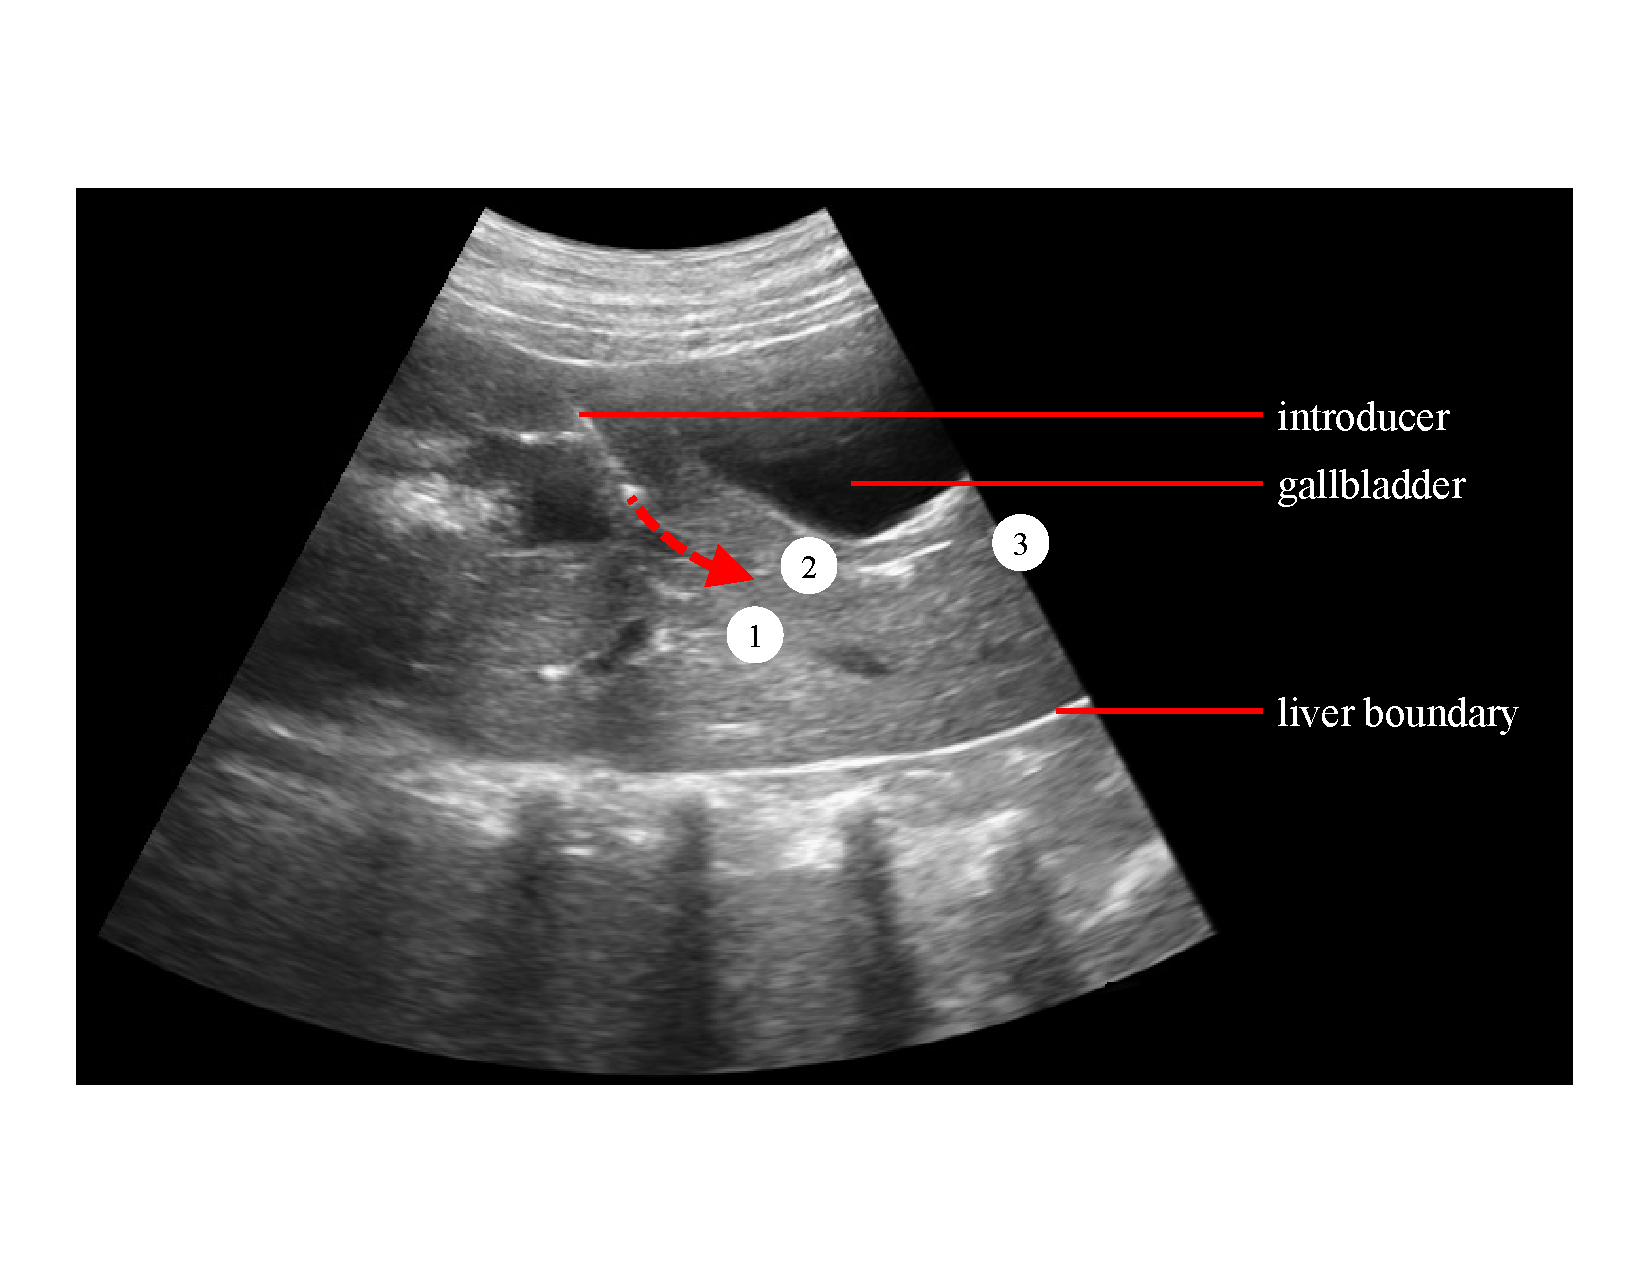
\includegraphics[width = \columnwidth]{./Images/Chapter5/CadaverTargetsUS/CadaverTargetsUS.pdf}%
\caption[Entry vector, targets and obstacles in cadaver liver]{Entry vector, targets and obstacles in cadaver liver. Three fiducials (numbered) were implanted around the gallbladder to provide targets for closed-loop needle steering. The targets were not all located within the imaging plane, and locations are approximate. The introducer needle and approximate initial path of the steerable needle are indicated, as are the gallbladder and liver boundary. }
\label{fig:CadaverSetup}
\end{figure} 




\section{Results}
\label{sec:HumanInTheLoopResults}

\subsection{Quantification of Process and Measurement Noise}
Across 517 samples of process noise, the mean position error (in millimeters) and mean orientation error (in degrees) were \[{\overline{p}_{w}} = \begin{bmatrix} 0.03 &-0.17 &0.01 \end{bmatrix}^{\text{T}}, {\overline{r}_{w}} = \begin{bmatrix} 0.18 &-0.03 &0.08 \end{bmatrix}^{\text{T}}.\] To find the best-fit zero-mean Gaussian distribution to the process noise, we again reflected the measured noise vectors, resulting in a sample covariance of
\begin{align*}
{\hat{Q}} = \begin{bmatrix} 
\phantom{-}0.16 & \phantom{-}0.02 	&-0.04 & -0.01 & \phantom{-}0.03 & \phantom{-}0.06\\
\phantom{-}0.02 & \phantom{-}0.16 & -0.02 & -0.05 & \phantom{-}0.03 & \phantom{-}0.01 \\ 
-0.04 & -0.02 & \phantom{-}0.46 & -0.10 & \phantom{-}0.01 & -0.03 \\
-0.01 & -0.05 & -0.10 & \phantom{-}0.24 & \phantom{-}0.01 & \phantom{-}0.02 \\
\phantom{-}0.03 & \phantom{-}0.03 & \phantom{-}0.01 & \phantom{-}0.01 & \phantom{-}0.05 & \phantom{-}0.03 \\
\phantom{-}0.06 & -0.01 & -0.03 & \phantom{-}0.04 & \phantom{-}0.03 & \phantom{-}0.24\\ 
\end{bmatrix}.
\end{align*}

In the measurement noise experiment, we again assumed the mean of repeated localization at each tip pose was the true needle pose.
\begin{align*}
{\hat{R}} = \begin{bmatrix} 
\phantom{-}2.29 & \phantom{-}1.58 & \phantom{-}2.51 \\ 
\phantom{-}1.58 & \phantom{-}6.97 & \phantom{-}2.19 \\ 
\phantom{-}2.51 & \phantom{-}2.19 & \phantom{-}11.4 \\ 
\end{bmatrix}.
\end{align*}

\subsection{Accuracy of Estimation Scheme}
Over 5199 data points, mean estimator error was 4.6~mm.


\begin{figure}[!t]
\centering
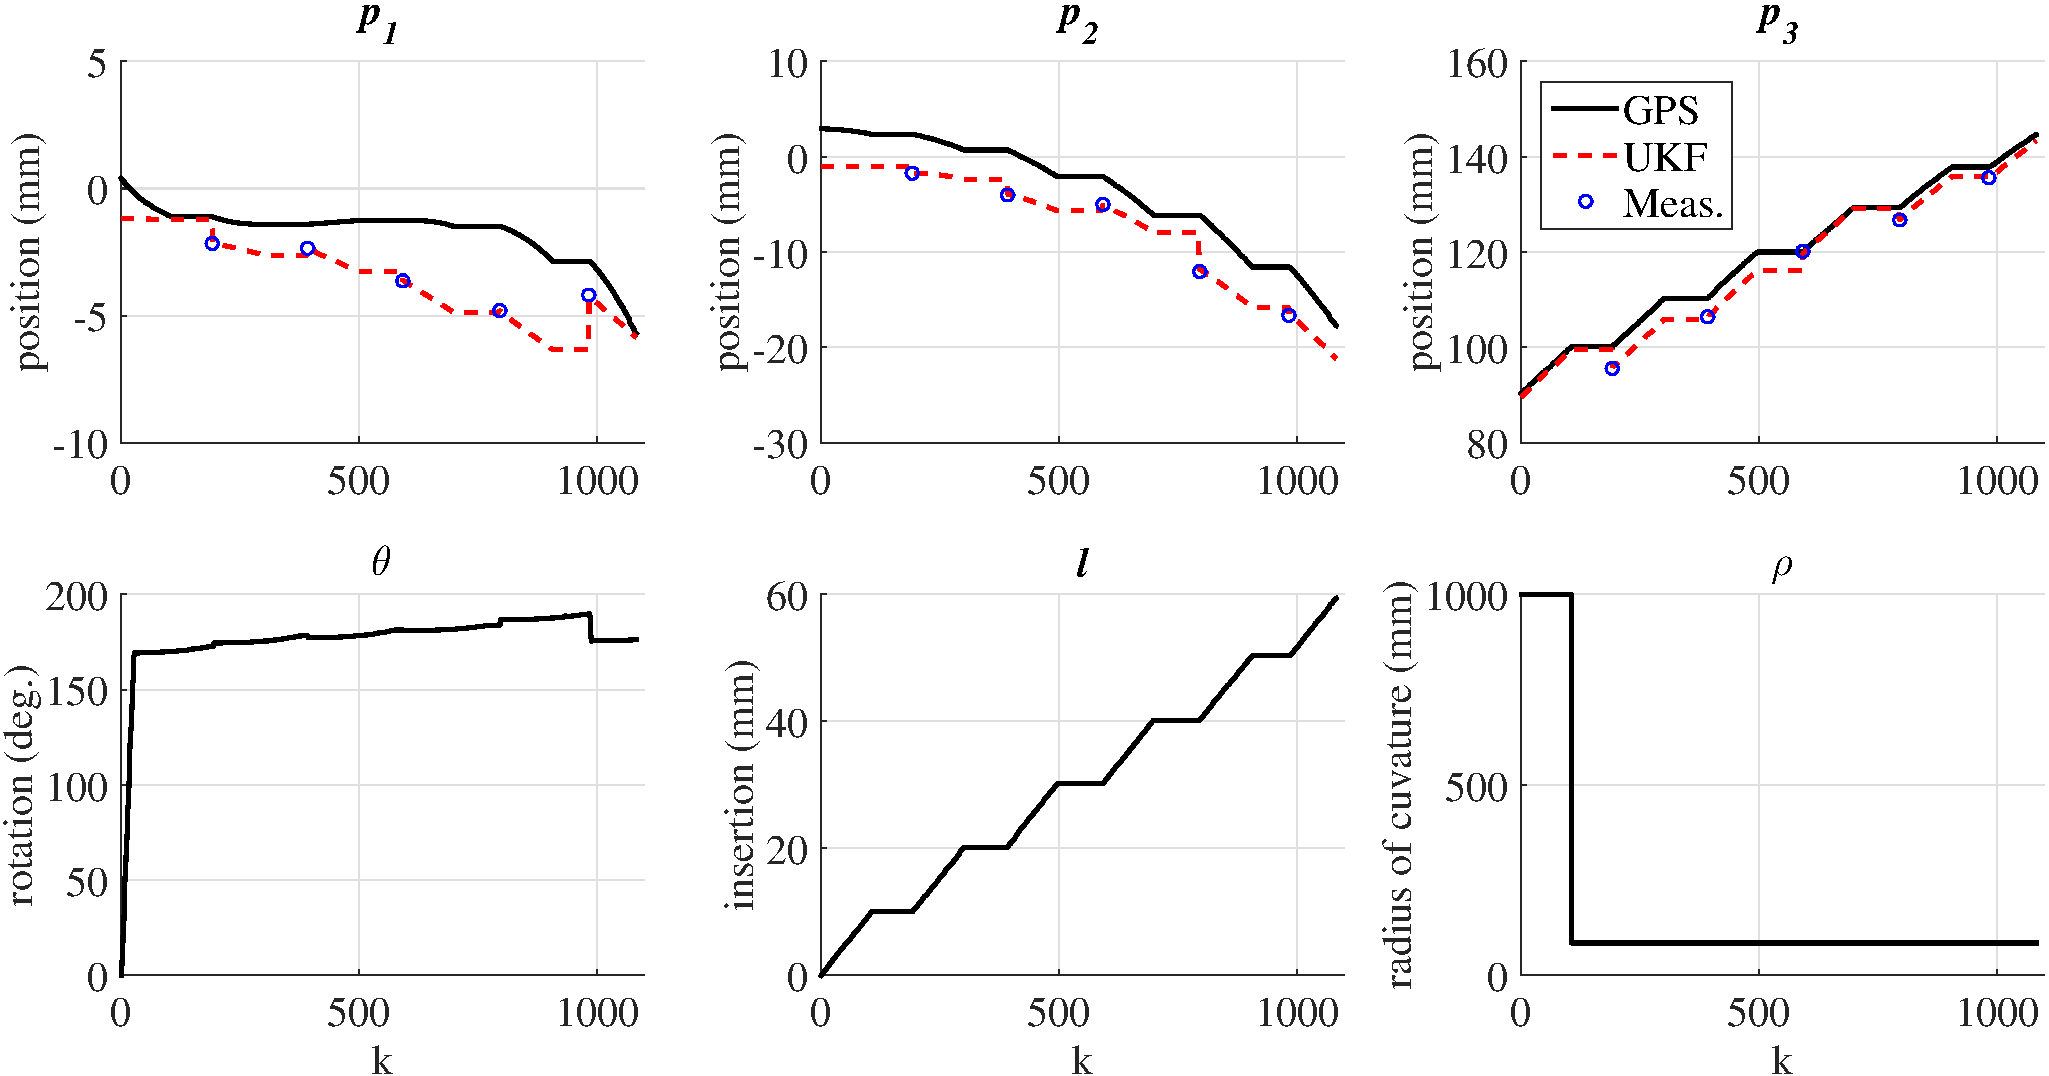
\includegraphics[width = \columnwidth]{./Images/Chapter5/UKFAccuracy/UKFAccuracy.pdf}%
\caption[UKF accuracy results]{UKF estimation scheme accuracy results. Comparison of calibrated and filtered electromagnetic tracker position (GPS) with estimator position (UKF). Measurements are also indicated. Robot joint variables ($\theta$, $l$) and radius of curvature $\rho$ inputs to the model are also shown. For UKF updates, $\rho$ is set to 1000~mm while the needle is inside the introducer sheath. }
\label{fig:GUI}
\end{figure}  

\subsection{Simulated Clinical Steering Experiments}

%!TEX root = PhD_Thesis.tex
\chapter[Conclusions and Future Work]{Conclusions and Future Work}
This dissertation has presented the design, implementation and experimental validation of methods for ultrasound-image-guided needle steering in percutaneous ablation of liver tumors, including (1) a method for segmenting steerable needles from 3D Doppler ultrasound data, (2) an articulated-tip steerable needle design that achieves clinically useful curvature in liver tissue, (3) an estimation scheme that allows infrequent noisy ultrasound measurements to be used for closed-loop control, and (4) an interface and system design that allows manual teleoperation of a steerable needle using freehand 3D ultrasound. 

\section{Segmentation}
In Chapter 2, we described using ultrasound Doppler imaging, in combination with high-frequency low-amplitude vibration of a steerable needle, to greatly simplify a challenging segmentation problem. Using the Doppler method, unsophisticated image processing methods can localize the needle with runtimes of milliseconds per image, and error on the order of 1~mm to 2~mm for relevant needle configurations. This segmentation algorithm has been shown to be robust to curvature, image orientation, and vibration frequency. Experiments in \textit{ex vivo} liver tissue have demonstrated that this method is accurate to within 1.2~mm of manual segmentation on average. Combining this segmentation method with a simple replanning-type control algorithm allows a needle steering robot to reach a simulated target with an average error below 2~mm. 

There are several potential directions for improvement of the Doppler segmentation method. Information on mechanical properties of the needle, such as minimum bending radius, could be used to improve the initial 2D segmentation, for example by limiting the search region for the needle cross section based on the maximum possible needle curvature. Combining data from multiple ultrasound scan modes (\textit{e.g.}, Doppler data, B-mode data, RF scanline data, and elastography data) could also potentially improve the accuracy and consistency of segmentation. For example, the Doppler data could be interpreted as a highlighter, allowing a more costly analysis of the B-mode data inside a region of interest. A preliminary implementation of this concept showed promising results, with millisecond runtimes and sub-millimeter accuracy~\cite{Greer2014}. The characteristics of the Doppler response might be improved by vibrating the needle tip itself, rather than the proximal shaft of the needle. One approach would be to place a small magnet in the shaft of the needle, and apply an alternating magnetic field using an electromagnet outside the body. A preliminary implementation of this concept increased the Doppler response at the tip of the needle compared to base vibration~\cite{Cabreros2014}.

\section{Needle Design and Curvature}
In Chapter 3, we examined the ability of bent-tip steerable needles to follow clinically relevant curved paths in liver tissue. An analysis of contrast-enhanced CT data was completed to define a procedure-specific requirement for needle curvature in ablation of liver tumors. This study showed that radius of curvature below 50~mm is necessary to reach the majority of the liver volume without injuring the liver capsule or major vasculature. A simplified FE model of bent-tip needle steering suggested that selection of bent-tip geometry could improve needle curvature to acceptable levels. This was confirmed by experiments in \textit{ex vivo} porcine liver tissue. Specifically, with tip length $l =$~12~mm and tip angle $\alpha =$~45~degrees, we found average radius of curvature to be below 50~mm in liver tissue, which is a significant improvement for a 0.8-mm tubular Nitinol needle compared to values reported in the literature. We also described the design of an articulated-tip steerable needle, which uses a miniaturized cable-driven rotary joint to articulate the needle tip between straight and bent configurations. This design allows the needle to have a more asymmetric tip, which results in better curvature, while the straight configuration also allows the needle to pass through an introducer sheath and rotate without extensive tissue deformation. Experimental validation testing demonstrates that the articulated-tip needle is able to achieve tighter curvature in liver tissue than comparable existing bent-tip needles. 

Although the articulated-tip design showed promising results in biological tissue, two main problems with needle design remain to be solved. The first problem is the robustness of the articulated design, which will need to be improved before such needles can be applied in a cadaver or animal model. As discussed in Chapter 3, the current plastic hinges fail too frequently to be applied in simulated clinical testing. Micromachining or additive manufacturing methods should be able to produce more robust metal hinges. Indeed, we explored such methods, but were unable to produce an acceptable prototype before moving on to the system testing described in Chapter 5. This led to the use of Nitinol flexure tips with exaggerated geometry. The second issue is the integration of a functional ablation element into the steerable needle. Since the needle lumen is currently only 0.5~mm in diameter, the most likely technologies for integration are alcohol ablation and microwave ablation.  

Another interesting issue for future consideration is whether existing kinematic models of needle steering, such as the unicycle and bicycle models~\cite{Park2005,Webster2006}, accurately capture the behavior of tightly curving steerable needles in tissue, as described in Chapter~3. With tighter curvature there is more relaxation of the surrounding tissues and more deviation from the ideal piece-wise circular paths, as seen in Fig.~\ref{fig:InsertAndTurn}.

\section{UKF Estimation Scheme}
In Chapter 4, we described a recursive estimation approach based on an unscented Kalman filter. Experimental measurement of the variability of asymmetric-tip needle steering in \textit{ex vivo} biological tissue was completed in order to formulate the UKF. Results in simulations and bench-top testing showed this filter allows a needle steering robot autonomously position the needle tip in a small workspace, with average error of about 2~mm.

In our current implementation, the UKF only receives feedback after a complement measurement of the steerable needle's tip pose, either through an automatic segmentation or manual localization. This currently requires a complete ultrasound sweep of the needle, with many images processed to yield only one measurement. Interestingly, all images of the needle's shaft do provide some information on the tip's pose. In future work, it might be possible to construct a single probabilistic framework which would incorporate each ultrasound frame containing the needle shaft as a measurement in order to refine the tip pose estimate.

\section{Human-in-the-Loop Control} 
In Chapter 5, we described human-in-the-loop control of a needle steering robot, using freehand 3D ultrasound imaging to define targets and provide control feedback. The system described in this chapter combined our methods for imaging, needle design, and estimation, in what we believe to be a clinically realistic implementation. 

(Suggestions for future work after seeing cadaver and final bench results.)


\bibliographystyle{IEEEtran}
\bibliography{Adebar_Dissertation}
\end{document}
